\documentclass[a4paper,10pt]{report}

% Load ``float'' before ``hyperref`` before ''algorithm``
% Note: ''algorithm`` would load ''float`` by itself
\usepackage{float}
\usepackage[pagebackref,hyperindex=true]{hyperref}

\usepackage{amsmath}
\usepackage{amssymb}
\usepackage{amsfonts}
\usepackage{amsopn}
\usepackage{braket}
\usepackage{bbm}
\usepackage{dsfont}
\usepackage{kpfonts}
% \usepackage{mathabx}

\parindent=0cm


% Various new commands that ease typesetting math even further
% \newcommand{\assign}{\ensuremath{\coloneq}}
% \newcommand{\rassign}{\ensuremath{\eqcolon}}
\newcommand{\assign}{\ensuremath{:=}}
\newcommand{\rassign}{\ensuremath{=:}}

\newcommand{\of}[1]{\ensuremath{\left( #1 \right)}}
\newcommand{\ofs}[1]{\ensuremath{\left( #1 \right)}}

\newcommand{\norm}[1]{\ensuremath{\| #1 \|}}

\newcommand{\tmop}[1]{\ensuremath{\operatorname{#1}}}

\newcommand{\id}{\ensuremath{\mathds{1}}}
% \newcommand{\id}{\ensuremath{I}}


\newcommand{\conj}[1]{\ensuremath{\overline{#1}}}

\newcommand{\T}{\ensuremath{{}^{\textnormal{T}}}}
\newcommand{\herm}{\ensuremath{{}^{\textnormal{H}}}}

\newcommand{\ft}[1]{\ensuremath{\mathcal{F}\left(#1\right)}}
\newcommand{\ift}[1]{\ensuremath{\mathcal{F}^{-1}\left(#1\right)}}

\newcommand{\fft}[1]{\ensuremath{\mathtt{FFT}\left(#1\right)}}
\newcommand{\ifft}[1]{\ensuremath{\mathtt{IFFT}\left(#1\right)}}

\newcommand{\dotp}[2]{\ensuremath{\langle #1 , #2 \rangle}}

\newcommand{\bigO}[1]{\ensuremath{\mathcal{O}\left( #1 \right)}}

\newcommand{\mat}[1]{\ensuremath{\mathbf{#1}}}

% multi-indices
\newcommand{\mindex}[1]{\ensuremath{\underline{#1}}}

\newcommand{\laplace}{\ensuremath{\operatorname{\Delta}}}

% EOF

\usepackage{graphicx}
\usepackage{subcaption}
\usepackage{asymptote}
\usepackage{tikz}
\usetikzlibrary{shapes,arrows}

\usepackage{algorithm}
\usepackage{algorithmic}

\usepackage{color}
\usepackage{relsize}
\usepackage[scaled=0.8]{beramono}
\usepackage{listings}

\definecolor{gray}{gray}{0.55}

% Python Code macro ------------------------------------------------------------

\newcommand{\python}[1] {
  \lstset{language=python,
          basicstyle=\smaller,
          basewidth=0.58em,
          columns=fixed,
          tabsize=2,
          fontadjust=true,
          frame=l,
          xleftmargin=4.2pt,
          numbers=left,
          stepnumber=2,
          breaklines=true,
          breakindent=0pt,
          prebreak=\mbox{\tiny$\searrow$},
          postbreak=\mbox{{\color{gray}$\cdots$}},
          keywordstyle=\bfseries,
          keywords={access,and,break,class,continue,def,del,elif ,else,
          except,exec,finally,for,from,global,if,import,in,is,
          lambda,not,or,pass,print,raise,return,try,while,
          True, False, None, self, from, import, as},
          numberstyle=\color{gray},
          commentstyle=\color{gray},
          stringstyle=\textit,
          showstringspaces=false,
        }
  \lstinputlisting{#1}
}

% C++ Code macro ---------------------------------------------------------------

\newcommand{\cpp}[1] {
  \lstset{language=c++,
          basicstyle=\smaller,
          basewidth=0.58em,
          columns=fixed,
          tabsize=2,
          fontadjust=true,
          frame=l,
          xleftmargin=4.2pt,
          numbers=left,
          stepnumber=2,
          breaklines=true,
          breakindent=0pt,
          prebreak=\mbox{\tiny$\searrow$},
          postbreak=\mbox{{\color{gray}$\cdots$}},
          numberstyle=\color{gray},
          commentstyle=\color{gray},
          stringstyle=\textit,
          showstringspaces=false,
        }
  \lstinputlisting{#1}
}

% Gnu R Code macro -------------------------------------------------------------

\newcommand{\gnuR}[1] {
  \lstset{language=R,
          basicstyle=\smaller,
          basewidth=0.58em,
          columns=fixed,
          tabsize=2,
          fontadjust=true,
          frame=l,
          xleftmargin=4.2pt,
          numbers=left,
          stepnumber=2,
          numberstyle=\color{gray},
          commentstyle=\color{gray},
          stringstyle=\textit,
          showstringspaces=false,
          literate={<-}{{$\leftarrow$}}1 {~}{{$\sim$}}1,
          escapeinside={(*}{*)}
        }
  \lstinputlisting{#1}
}


\usepackage[utf8x]{inputenc}
\usepackage{cancel}
\usepackage{url}
\usepackage{placeins}
\usepackage{microtype}

% Links in pdf
\usepackage{color}
\newcommand{\blue}{ \color{blue} }
\definecolor{linkcol}{rgb}{0,0,0.4}
\definecolor{citecol}{rgb}{0.5,0,0}

\hypersetup
{
colorlinks=true,
linkcolor=linkcol,
citecolor=citecol,
urlcolor=linkcol
}

% nicer backref links
\renewcommand*{\backref}[1]{}
\renewcommand*{\backrefalt}[4]{%
\ifcase #1 %
(Not cited.)%
\or
(Cited on page~#2.)%
\else
(Cited on pages~#2.)%
\fi}
\renewcommand*{\backrefsep}{, }
\renewcommand*{\backreftwosep}{ and~}
\renewcommand*{\backreflastsep}{ and~}

\parindent 0cm

\newcommand{\clearemptydoublepage}{\newpage{\pagestyle{empty}\cleardoublepage}}


\begin{document}

\begin{titlepage}
	\begin{center}

		\hfill

		\vspace{2cm}

		{\huge \textsc{Time Propagation\\ of Quantum Wave Packets\\[10pt]}}
		{\Large \textsc{an efficient implementation in C++\\[10pt]}}

		\vspace{1cm}

		{\Large{Bachelor Thesis}}

		\vspace{1cm}

		{\emph{written by}} \\
		{
			Matthias Untergassmair
		}

		\vspace{1cm}

		{\emph{advised by}} \\
		{
			Raoul Bourquin
		}

		\vspace{1cm}

		{\emph{supervised by}} \\
		{
			Dr. Vasile Gr\u{a}dinaru\\
			Prof. Dr. Ralf Hiptmair
		}
		
		\vfill

		Seminar for Applied Mathematics\\
		ETH Zurich

		\vspace{.5cm}

		\emph{{Fall semester 2016}}

		\vspace{.5cm}

		
\includegraphics[width=0.5\linewidth]{figures/eth-logo.pdf}

	\end{center}

\end{titlepage}


\clearemptydoublepage

\tableofcontents
\listoffigures
%\listofalgorithms

\clearemptydoublepage

\begin{chapter}{Introduction}
\label{ch:introduction}

In this chapter we introduce the fundamental physical and mathematical ideas and
structures on which the other chapters build. The central objects here are the
time-dependent Schrödinger equation and a non-adiabatic potential.


\section{The time-dependent Schrödinger equation}

Time-dependent problems in quantum physics are governed by the time-dependent
Schrödinger equation

\begin{equation} \label{eq:basics_tdse_simple}
  i \hbar \frac{\partial}{\partial t} \Ket{\varphi} = H \Ket{\varphi} \,.
\end{equation}

The Hamiltonian of the system in consideration is given by $H$, and the function
$\varphi\ofs{x,t}$ represents the wavefunction dependent on position $x$ and
time $t$. In $d$ space dimensions this is

\begin{align*}
  \varphi : \mathbb{R}^d \times \mathbb{R} & \rightarrow \mathbb{C} \\
                       \left( x, t \right) & \mapsto \varphi\ofs{x,t} \,.
\end{align*}

There are various mathematical restrictions on what is a valid wavefunction. For
example $\varphi$ has to be square-integrable. Most of these preconditions have
little importance for us.

\section{Semi-classical scaling}

We use the semiclassical scaling, where $\varepsilon > 0$ is a real parameter
\footnote{Other authors use $\varepsilon$ or even $\hbar$ (without its physical
meaning and value) for the quantity we denote by $\varepsilon^2$.}. The equation
still keeps its mathematical form

\begin{equation} \label{eq:basics_tdse_semi}
  i \varepsilon^2 \frac{\partial}{\partial t} \Ket{\psi} = H \Ket{\psi} \,.
\end{equation}

It's well known that we get the classical dynamics from the limit $\hbar \rightarrow 0$.
The same holds of course for the semiclassical parameter $\varepsilon$ and for bigger
$\varepsilon$ we get an increasing amount of quantum effects.

The Hamiltonian operator $H$ is composed of two parts, the kinetic operator $T$
and the potential operator $V$. Thus we can split $H$ as $H = T + V$ with the
following definitions for both operators

\begin{equation} \label{eq:basics_def_ops}
\begin{split}
  T & \assign - \frac{1}{2} \varepsilon^4 \frac{\partial^2}{\partial x^2} \\
  V & \assign V\ofs{x} \,.
\end{split}
\end{equation}

The mass $m$ which is present in the common definition of the kinetic operator
is included in the parameter $\varepsilon$. The potential is a real valued
function depending only on space but not on time. This static potential results
from the Born-Oppenheimer approximation for the electronic structure problem.
For a more detailed theoretical background see for example reference
\cite{S_Teufel}. Assume the potential is given by

\begin{equation} \label{eq:basics_potential_function}
\begin{split}
  V : \mathbb{R}^d & \rightarrow \mathbb{R} \\
                 x & \mapsto V\ofs{x}
\end{split}
\end{equation}

then this allows us to solve the Schrödinger equation by separation of variables
and obtain an analytical result for the time propagation of a quantum state $\Ket{\psi\ofs{t}}$

\begin{equation} \label{eq:basics_analytic_time_propagation}
  \Ket{\psi\ofs{t}} = e^{- \frac{i}{\varepsilon^2} H t } \Ket{\psi\ofs{0}} \,.
\end{equation}

The solutions to this time propagation have fine details. A typical wavepacket
is highly oscillatory with a wavelength $\bigO{\varepsilon^2}$ localized in space
with $\bigO{\varepsilon^2}$ and moving with a velocity of $\bigO{1}$. This tiny
structures are a challenge for the algorithms simulating them. We would need a very
fine grid and thus a huge bunch of grid nodes.


\section{Non-adiabatic potentials, avoided crossings}

Non-adiabatic potentials are potentials that consist of multiple energy levels.
These energy levels may intersect each other, but we are interested in a situation
that is called an \emph{avoided crossing}. That is, the two energy surfaces always
stay in a minimal distance. We call this distance the energy gap and denote it by
$\delta$. A very simple example of such an avoided crossing with only two energy
levels is shown in figure \ref{fig:example_avoided_crossing}.

\begin{figure}
  \centering
  \begin{asy}[width=\the\linewidth]
import graph;

real left = -2;
real right = 2;

real delta = 0.15;

real lambda0(real x) { return sqrt(tanh(x)^2+delta**2)/2; }
real lambda1(real x) { return -sqrt(tanh(x)^2+delta**2)/2; }

xaxis("$x$",Arrow);
yaxis("$y$",Arrow);

draw(graph(lambda0,left,right,operator ..),blue);
draw(graph(lambda1,left,right,operator ..),blue);

real u = lambda0(0);
real l = lambda1(0);

pair s = (0,l+0.05*delta);
pair e = (0,u-0.05*delta);

draw("$\delta$", s--e, red, Arrows, PenMargins);

real u = lambda0(2);
pair l1 = (1,u);

real u = lambda1(2);
pair l0 = (1,u);

label("$\lambda_1(x)$",l1+S);
label("$\lambda_0(x)$",l0+N);
\end{asy}

  \caption{Example of an avoided crossing of two energy levels.}
  \label{fig:example_avoided_crossing}
\end{figure}

Based on the class of physical potential in consideration we have a strict monotone
order of the eigenvalues for all $x$ in our space \footnote{This is a fairly strong
assumption that can be replaced by much weaker formulations more suitable for mathematical
analysis. But for our purpose it is sufficient and these details don't really matter.}

\begin{equation}
  \lambda_0\ofs{x} > \lambda_1\ofs{x} > \ldots > \lambda_{N-1}\ofs{x} \qquad \forall x \,.
\end{equation}

This global consistent order allows us to sort the eigenvalues and the corresponding
eigenvectors uniquely in decreasing order.

For a more elaborate study of the mathematical details and a classification of
different types of avoided crossings see reference \cite{H_classification}.

We are now interested in what happens with an incoming wavepacket $\Ket{\psi}$ while
it traverses the narrow part. The magnitude $\delta$ of the energy gap plays an
important role in this process.

\section{A vector of states}

For the study of avoided crossings of the energy levels we are interested in vector valued
states $\Ket{\Psi}$. Each component of this vector represents a part of the wavefunction
being on the corresponding energy surface.

To describe the dynamics of these states, we need to generalize the Schrödinger equation
to a vector valued version. This is not difficult to do, basically the extended equation looks
exactly like \eqref{eq:basics_tdse_semi} but with the difference that $H$ is a matrix now.
Let's write down this in more detail because we will refer to it over and over again.

Assume we deal with $N$ different states hence $\Ket{\Psi}$ consists of $N$ components
$\varphi_i \ofs{x}$. And the Hamiltonian becomes a real valued symmetric $N \times N$
matrix. This gives the following expression for the time-dependent Schrödinger equation

\begin{equation} \label{eq:basics_tdse_vector}
  i \varepsilon^2 \frac{\partial}{\partial t} \Ket{ \begin{pmatrix}
                                                   \varphi_0 \\
                                                   \vdots \\
                                                   \varphi_{N-1}
                                                 \end{pmatrix}
                                               }
  =
  \begin{pmatrix}
    {} & {} & {} \\
    {} & H  & {} \\
    {} & {} & {} \\
  \end{pmatrix}
  \underbrace{
  \Ket{ \begin{pmatrix}
          \varphi_0 \\
          \vdots \\
          \varphi_{N-1}
        \end{pmatrix}
      }}_{\Ket{\Psi}} \,.
\end{equation}

\section{The potential}

In the case of a non-adiabatic potential with multiple energy levels,
the potential $V$ becomes a matrix. We assume that $V$ depends on space $x$
but not on time $t$, thus it is time-independent.

The matrix representing $V$ is symmetric and with entries $v_{i,j} \equiv v_{j,i} \in \mathbb{R}$. We may
write a general unspecified potential as

\begin{equation} \label{eq:general_potential_matrix}
  V\ofs{x} \rassign
  \begin{pmatrix}
    v_{0,0}\ofs{x} & \cdots & v_{0,N-1}\ofs{x} \\
    \vdots         &        & \vdots \\
    v_{N-1,0}\ofs{x} & \cdots & v_{N-1,N-1}\ofs{x}
  \end{pmatrix}
\end{equation}

where each of the matrix entries $v_{i,j}\ofs{x}$ is a real valued function

\begin{align*} \label{eq:matrix_potential_function_entry}
  v_{i,j} : \mathbb{R}^d & \rightarrow \mathbb{R} \\
                       x & \mapsto v_{i,j}\ofs{x}
\end{align*}

on its own. These functions are assumed to be smooth.

\subsection{Diagonalization of the potential}
\label{sec:diagonalize_potential}

We are much more interested in the potential's eigenvalues which are the energy
levels of our system. A well known result from linear algebra tells us that
symmetric matrices always have only real eigenvalues. Therefore we can diagonalize
this matrix and obtain pure real eigenvalues $\lambda_i\ofs{x}$ that depend on the
space variable $x$.

The diagonalization itself is performed by orthogonal matrices, the same theorem
as above guarantees that we have a full set of orthogonal eigenvectors $\nu_i\ofs{x}$
which depend of course on $x$ too.

Given the full set of eigenvalues $\lambda_0\ofs{x}, \ldots, \lambda_{N-1}\ofs{x}$
and the corresponding eigenvectors of $V\ofs{x}$ denoted by $\nu_0\ofs{x}, \ldots, \nu_{N-1}\ofs{x}$
the spectral decomposition of the potential's matrix reads

\begin{equation} \label{eq:general_spectral_transformation}
  \Lambda\ofs{x} = M^{-1}\ofs{x} V\ofs{x} M\ofs{x}
\end{equation}

where the matrix $\Lambda$ is diagonal with the eigenvalues $\lambda_i$ on its
diagonal. The transformation matrix $M$ is orthogonal and contains the
eigenvectors as columns

\begin{equation} \label{eq:general_transformation_matirx}
  M \assign
  \begin{pmatrix}
    \nu_0\ofs{x} & , \hdots , & \nu_{N-1}\ofs{x}
  \end{pmatrix} \,.
\end{equation}

\subsubsection{The special case for 2 energy levels}

A general potential that only contains two energy levels is given by a symmetric
two by two matrix. In this case we can write down the eigenvalues for the potential
in closed form. The following formulae are defined in more detail in \cite{H_T_semiclassical_2x2}.
Suppose the potential matrix is given by

\begin{equation}
  V\ofs{x} \assign
  \begin{pmatrix}
    v_1 &  v_2 \\
    v_2 & -v_1
  \end{pmatrix}
\end{equation}

with trace $\text{Tr}\ofs{V} = 0$. Then we define a $\theta$ as

\begin{equation}
  \theta \assign \frac{1}{2} \arctan \ofs{\frac{v_2}{v_1}} \,.
\end{equation}

For the numerical computation we have to use the \texttt{atan2} function to get
the signs correct. Finally we can write the two eigenvectors as

\begin{equation}
  \nu_0 \assign
  \begin{pmatrix}
    \cos\ofs{\theta} \\
    \sin\ofs{\theta}
  \end{pmatrix}
  \quad
  \nu_1 \assign
  \begin{pmatrix}
    -\sin\ofs{\theta} \\
    \cos\ofs{\theta}
  \end{pmatrix} \,.
\end{equation}

Obviously they are orthogonal and normed. Remember that if we sort the $\lambda_i$
we have to change the order of the eigenvectors
as well. It's not guaranteed that $\nu_0$ always belongs to $\lambda_0$.

\subsection{Basis transformations of states}
\label{sec:basis_transformations_of_states}

For various calculations later on we need to be able to transform states from and to
the eigenbasis. This is in principle a trivial process of linear algebra, but lets
briefly note the important points.

The transformation from the eigenbasis to the canonical basis will be important
when we set up the initial values for a simulation. Assume we have a wavefunction
$\Ket{\varphi^e}$ given in the eigenbasis. The transformed state in the canonical
basis is given by

\begin{equation}
  \Ket{\varphi^c} = M \Ket{\varphi^e}
\end{equation}

where $M$ contains the column vectors $\nu_i$.

The opposite transformation becomes important when evaluating observables. Given
a state $\Ket{\varphi^c}$ in the canonical basis, the image of the transformation
into the eigenbasis is

\begin{equation}
  \Ket{\varphi^e} = M\T \Ket{\varphi^c}
\end{equation}

where we simplified $M^{-1} = M\T$ for real orthogonal matrices.

\end{chapter}


\clearemptydoublepage

\begin{chapter}{Morse Expansion of Potentials}
In the algorithm for the Hagedorn wave packets it was necessary to split an arbitrary potential into a quadratic part and a remainder.
Hence, for an algorithm based on wave packets of Morse eigenfunctions, we have to perform a similar splitting into a Morse part and a remainder.
While in the harmonic case this can be quite easily done by just using the second order Taylor approximation of the potential, the case of the
Morse potential is more complex since it is anharmonic and in particular non-polynomial.\\

In the following we present and compare different methods to obtain the parameters for the Morse potential. The first naive approach, which tries to 
mimic the procedure in \cite{FGL_semiclassical_dynamics} is based on a local Taylor expansion of the target potential while the second uses a least-squares fit to
the target potential. It is important to note that we only need a locally good approximation of the target potential by a Morse potential, since
deviations are included in the potential remainder and, if not too big, taken care of in the final Galerkin approximation step of the time-stepping
algorithm.

A natural candidate for testing our splitting method is the Lennard-Jones potential
\begin{equation}
    \label{eq:LennardJonesPot}
    L(r):=\varepsilon\left[\left(\frac{r_m}{r}\right)^{12}-2\left(\frac{r_m}{r}\right)^{6} \right],
\end{equation}
which is also anharmonic and used to model molecular bonds. As one can see in Figure \ref{fig:LJPlots} 
it also looks very similar to the Morse potential .\\

In contrast to the Morse potential, however, the Lennard-Jones potential is not analytically solvable. The parameter $\varepsilon$ describes the depth of the potential while $r_m$ is the position of its minimum.\\

\begin{figure}[h!]
    \centering
     \subfloat[][]{
	\label{fig:LJPlot3_7}
	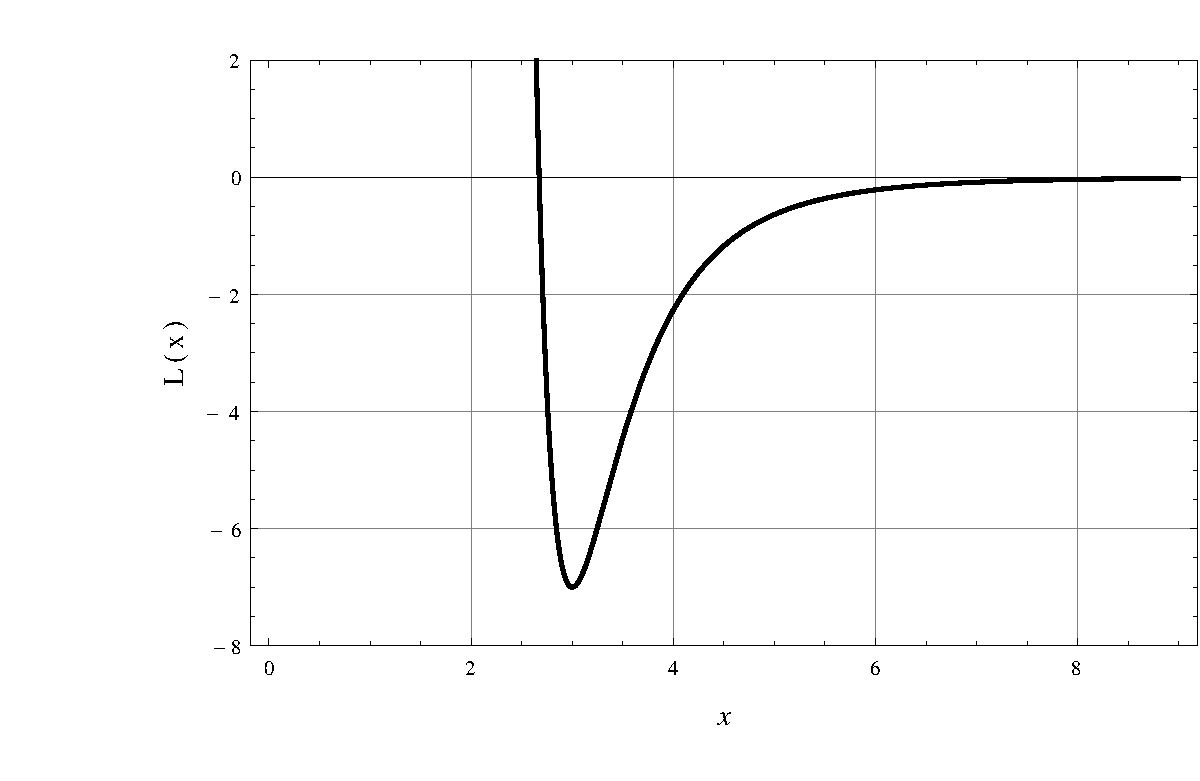
\includegraphics[width=0.5\linewidth]{./figures/LJPlots/LJ3_7.pdf}
    }
    \subfloat[][]{
	\label{fig:LJPlot2_4}
	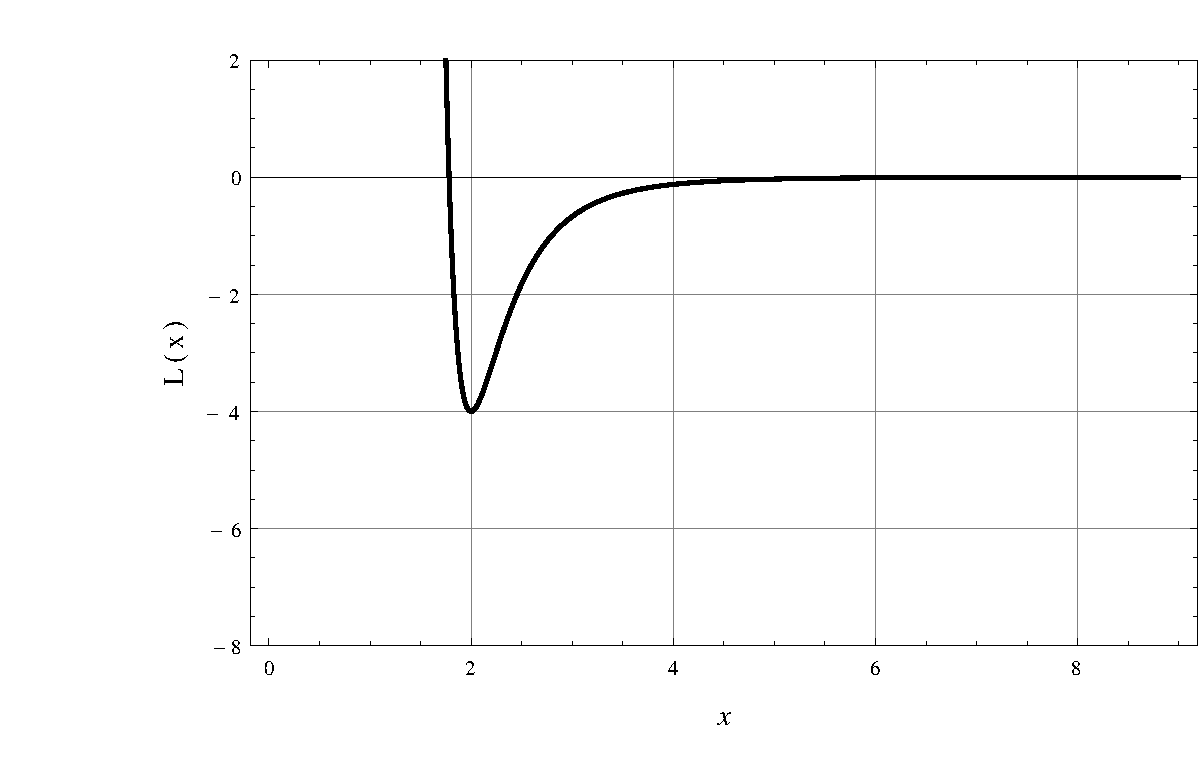
\includegraphics[width=0.5\linewidth]{./figures/LJPlots/LJ2_4.pdf}
    }\\

       \caption[Lennard-Jones Potential]{Plot of the Lennard-Jones potential for two different
	   parameter set. $r_m$ defines the position of the minimum and $\epsilon$ its depth.
    \subref{fig:LJPlot3_7} $r_m=2.0$ and $\epsilon=4.0$
    \subref{fig:LJPlot2_4} $r_m=3.0$ and $\epsilon=7.0$
    \label{fig:LJPlots}
    }

\end{figure}



\section{Taylor expansion} % (fold)
\label{sec:Non-Grid based methods}
From an algorithmic point of view it is of course desirable to have a set of closed form formulas for the the Morse parameters rather than having
to solve a large and possibly non-linear system of equations in every step of the algorithm. Thus, we first look if there is a straightforward way to
calculate the Morse potential parameters from locally available information about our target potential, that is the value of its derivatives.

\subsection{Coefficients of Taylor expansion} % (fold)
\label{sub:Coefficients of Taylor expansion}
To determine the three free parameters $x_0, V_0$ and $\beta$ we need three independent equations. We thus expand the Morse potential $M(x)$ to second
order which yields:
\begin{align}
	\begin{split}
    M(x)=&-2V_0e^{-\beta(q-x_0)}+V_0e^{-2(q-x_0)})\\
    &+2\beta V_0(e^{-\beta(q-x_0)}+e^{-2(q-x_0)})(x-q)\\
    &-\beta^2V_0(e^{-\beta(q-x_0)}+2V_0\beta^2e^{-2(q-x_0)})(x-q)^2+\bigO{(x-q)^3}
    \end{split}
\end{align}
Assuming that target potential $V(x)$ is at least $\mathcal{C}^2(\mathbb{R})$ we can compare coefficients and obtain the following non-linear
system:
\begin{align}
    \label{eq:TaylorParamsOrig}
    \begin{split}
    -2V_0e^{-\beta(q-x_0)}+V_0e^{-2\beta(q-x_0)}&=V(q):=P_1\\
    +2\beta V_0 e^{-\beta(q-x_0)}-2V_0\beta e^{-2\beta(q-x_0)}&=V'(q):=P_2\\
    -\beta^2V_0 e^{-\beta(q-x_0)}+2V_0\beta^2 e^{-2\beta(q-x_0)}&=\frac{V''(q)}{2}:=P_3
    \end{split}
\end{align}
With the substitution $A:=e^{-\beta(q-x_0)}$, this simplifies to the following system
of quadratic equations:
\begin{align}
    \begin{split}
	V_0(-2A+A^2)&=P_1\\
	2\beta V_0(A-A^2)&=P_2\\
	2\beta^2 V_0(-A+2A^2)&=P_3
    \end{split}
\end{align}
leading to the two solutions
\begin{align}
\beta&=\frac{-3P_2^2+\sqrt{9P_2^4-8P_3P_2^2P_1}}{4P_2P_1}\\
V_0^{(1,2)}&=\frac{\pm3P_2^4\pm8P_3^2P_1^2(\mp12P_3P_1\sqrt{9P_2^4-8P_3P_2^2P_1})}{\pm8P_3(P_2^2-P_3P_1)}\\
A^{(1,2)}&=\frac{\pm5P_2\mp4P_3P_1+\sqrt{P_2^2(9-P_2^2-8P_3P_1)}}{\pm4P_2^2-4P_3P_1}
\end{align}
which can then be subsequently solved for $x_0$.\\

Due to the quadratic nature of these equations,
we obtain two solutions, corresponding to the exact local expansion we are looking for and
a version that is mirrored either in $x$ or $y$-direction. Hence, for a general algorithm, 
additional steps must be employed to identify the correct one. Fits can be see in the following figure \ref{fig:MorseFitsTaylor}.


%Due to the non-linearity we cannot obtain an explicit expression for our parameters. Nevertheless, it would be possible to recast these equations as
%a root-finding problem and solve it numerically using Newton iteration for instance. However, for an arbitrary potential it is not clear whether
%a unique, physical solution exists and furthermore if the algorithm will converge to it. \\
%
%Another possibility is to simplify the expression by expanding the Morse potential around its minimum:
%\begin{equation}
%    \label{eq:MorseTaylor2nd}
%    -V_0+\beta^2V_0(x-x_0)^2+\bigO{(x-x_0)^3}
%\end{equation}
%By that choice we implicitly fix the former free parameter $x_0$ to the current mean location $q$ of the wave packet we wish to propagate.
%In that can case we can also find an easy expression for the coefficients of the Taylor expansion:
%\begin{equation}
%    \label{eq:MorseTaylorCoeff}
%    \frac{(-2+2^n)(-\beta)^nV_0}{n!},\quad n\in\mathbb{N}
%\end{equation}
%
%Comparing coefficients again with the expansion of the potential $V(x)$ around $q=x_0$ leads to the following simple set of equations:
%\begin{align}
%    \label{eq:TaylorParams}
%    \begin{split}
%	-V_0	    &=  V(x_0)\\
%        0	    &=  V'(x_0)\\
%	\beta^2V_0  &=	\frac{V''(x_0)}{2}
%    \end{split}
%\end{align}
%From that we can indeed easily derive expressions for our parameters $\beta$ and $V_0$:
%\begin{equation}
%    V_0=-V(x_0),\qquad \beta=\sqrt{\frac{-V''(x_0)}{2V(x_0)}}
%\end{equation}
%Naturally, the second equation in \eqref{eq:TaylorParams} came about by choosing $q=x_0$ to be the minimum of the Morse potential.
%This is problematic since it basically demands that the potential $V(x)$ is extremal in $x_0$ as well, which is of course not necessarily the case.
%Even though we only need a locally good Morse-like approximation to the potential we can see in the following figures \ref{fig:MorseFitsTaylor} that if the extremality
%condition is violated, the Morse approximation becomes useless. 
\begin{figure}[h!]
    \centering
%     \subfloat[][]{
%	\label{fig:Taylor090}
%	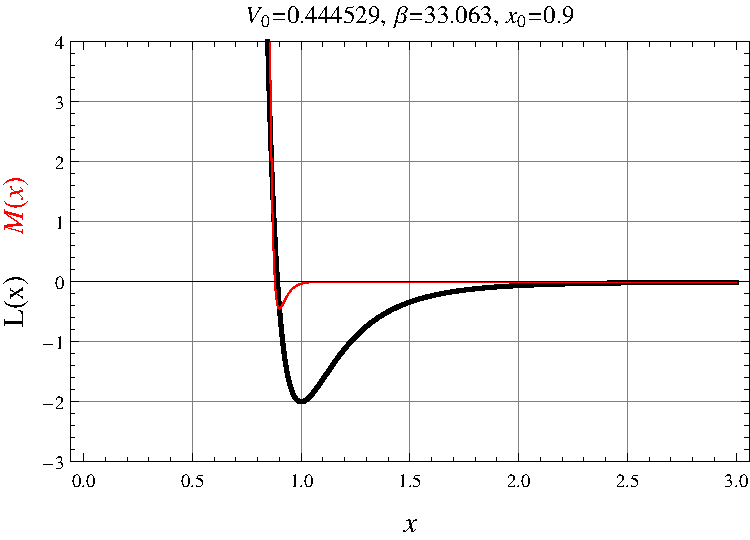
\includegraphics[width=0.5\linewidth]{./figures/MorseFitsTaylor/Taylor090.pdf}
%    }
%    \subfloat[][]{
%	\label{fig:Taylor100}
%	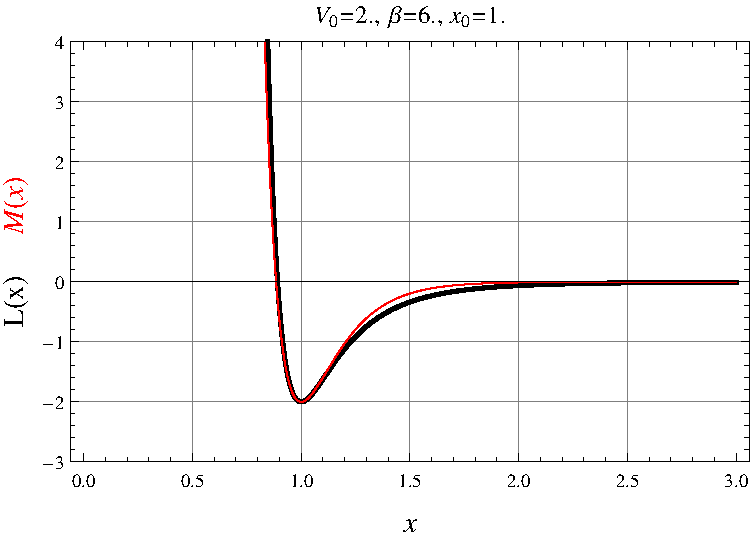
\includegraphics[width=0.5\linewidth]{./figures/MorseFitsTaylor/Taylor100.pdf}
%    }\\
%    \subfloat[][]{
%	\label{fig:Taylor105}
%	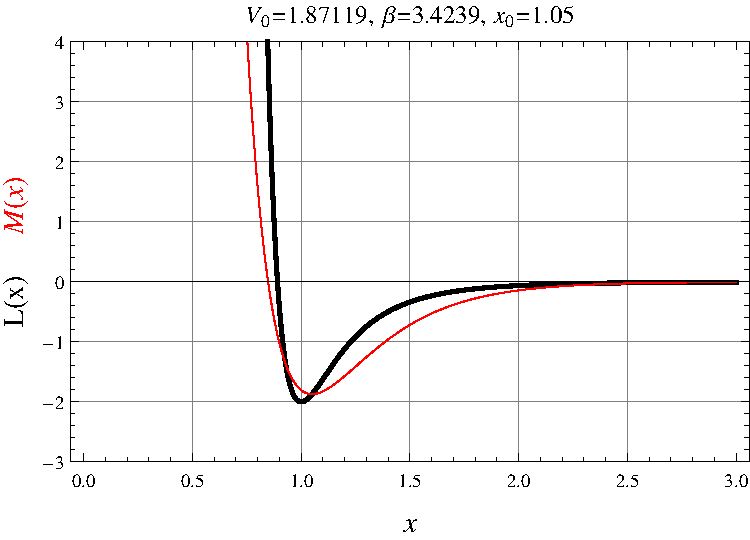
\includegraphics[width=0.5\linewidth]{./figures/MorseFitsTaylor/Taylor105.pdf}
%    }
%    \subfloat[][]{
%	\label{fig:Taylor110}
%	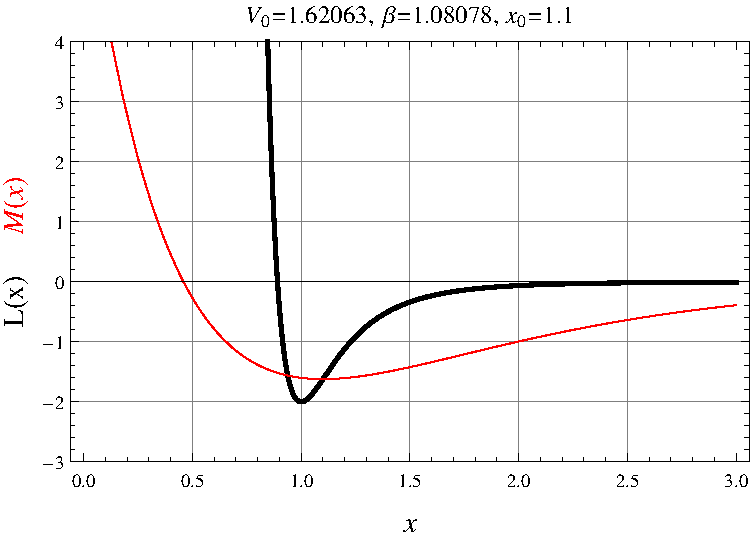
\includegraphics[width=0.5\linewidth]{./figures/MorseFitsTaylor/Taylor110.pdf}
%    }
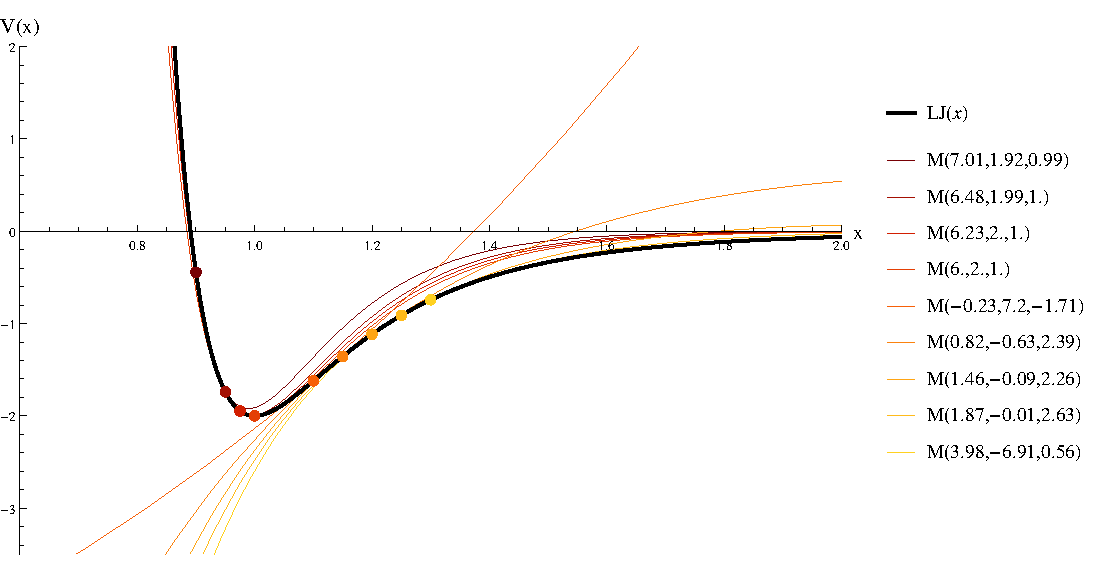
\includegraphics[width=1.2\linewidth]{./figures/MorseFitsTaylor/taylorfitsAll.pdf}
    \\

       \caption[Fits using Taylor series coefficient equations]{\textbf{Fits using Taylor series coefficient equations}:
	In the plots we see the results of fitting the Morse potential to a Lennard-Jones potential with $r_m=1.0$ and $\epsilon=2.0$.
	    \label{fig:MorseFitsTaylor}
    }

\end{figure}

% subsection Coefficients of Taylor expansion (end)

% section Least Square methods

\section{Least Square methods} % (fold)
\label{sec:LeastSquareMethods}
The basic problem of the previous approach is that we only use the information available at the point $q$ by a comparison to a polynomial approximation.
To obtain better results one has to explicitly minimize the error in the region of interest around $q$ which naturally leads to a least squares 
approach. For a given potential $V(x)$ one tries to find  Morse parameters $x_0, V_0$ and $\beta$ such that

\begin{equation}
    \label{eq:lstsqprob}
    S(x_0, V_0, \beta)=\sum_{i=1}^N[V(x_i)-M(x_i,x_0,V_0, \beta)]^2 
\end{equation}
becomes minimal. For simplicity, the sample points $\lbrace x_i\rbrace_{i=1}^N$ are chosen equidistant within a $\delta$-neighborhood around 
the current mean wave packet position $q$ while the current width wave packet parameter $Q$ might be a good indicator for choosing the size
of $\delta$. \\
Also the distribution of the sample points within that interval might be chosen more concentrated in the center of the interval or adapted
to other components of a potential Morse packet time-stepping algorithm. Depending on the quality of the fit one could already sample
the quadrature nodes for the Galerkin approximation in the last step of the algorithm.\\

For the test with the Lennard-Jones potential the Python routines \texttt{curve\_fit} and \texttt{leastsq} from the \texttt{scipy.optimize}
package were used. \\
% section Grid based methods (end)


\subsection{\texttt{curve\_fit}} % (fold)
\label{sub:curve_fit}
The function \texttt{curve\_fit} is actually just  a wrapper for \texttt{leastsq} but in the latter case one can also provide an analytical Jacobian while
\texttt{curve\_fit}, by default, estimates it. The underlying FORTRAN library \textbf{MINPACK} implements the Levenberg-Marquardt algorithm (LMA),
also known as damped least-squares method to solve the least squares problem \eqref{eq:lstsqprob}.\\
The results of these fits are shown in Figure \ref{fig:MorseFitsCurvefit}.

\begin{figure}[h!]
    \centering
%     \subfloat[][]{
%	\label{fig:CurveFit09}
%	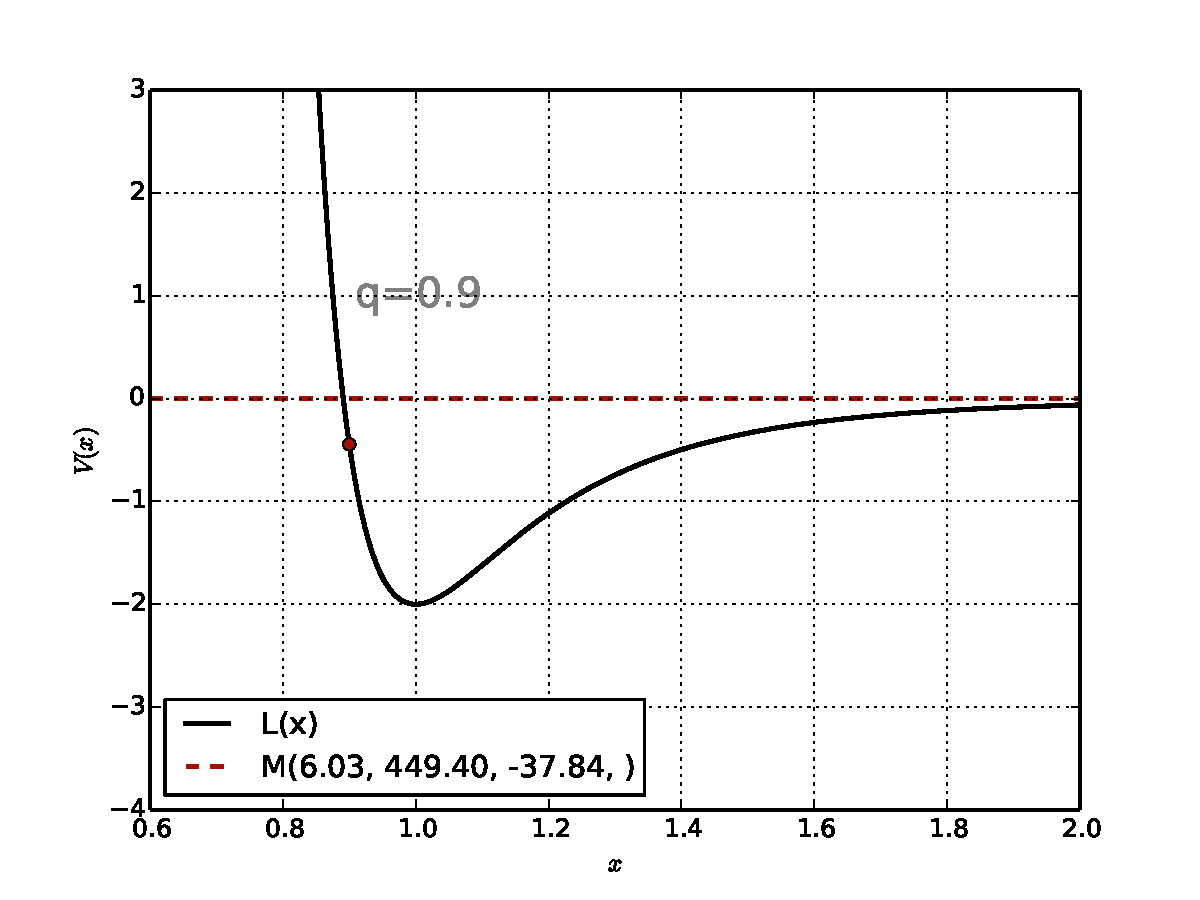
\includegraphics[width=0.5\linewidth]{./figures/MorseFitsCurvefit/curvefit09.pdf}
%    }
%    \subfloat[][]{
%	\label{fig:CurveFit095}
%	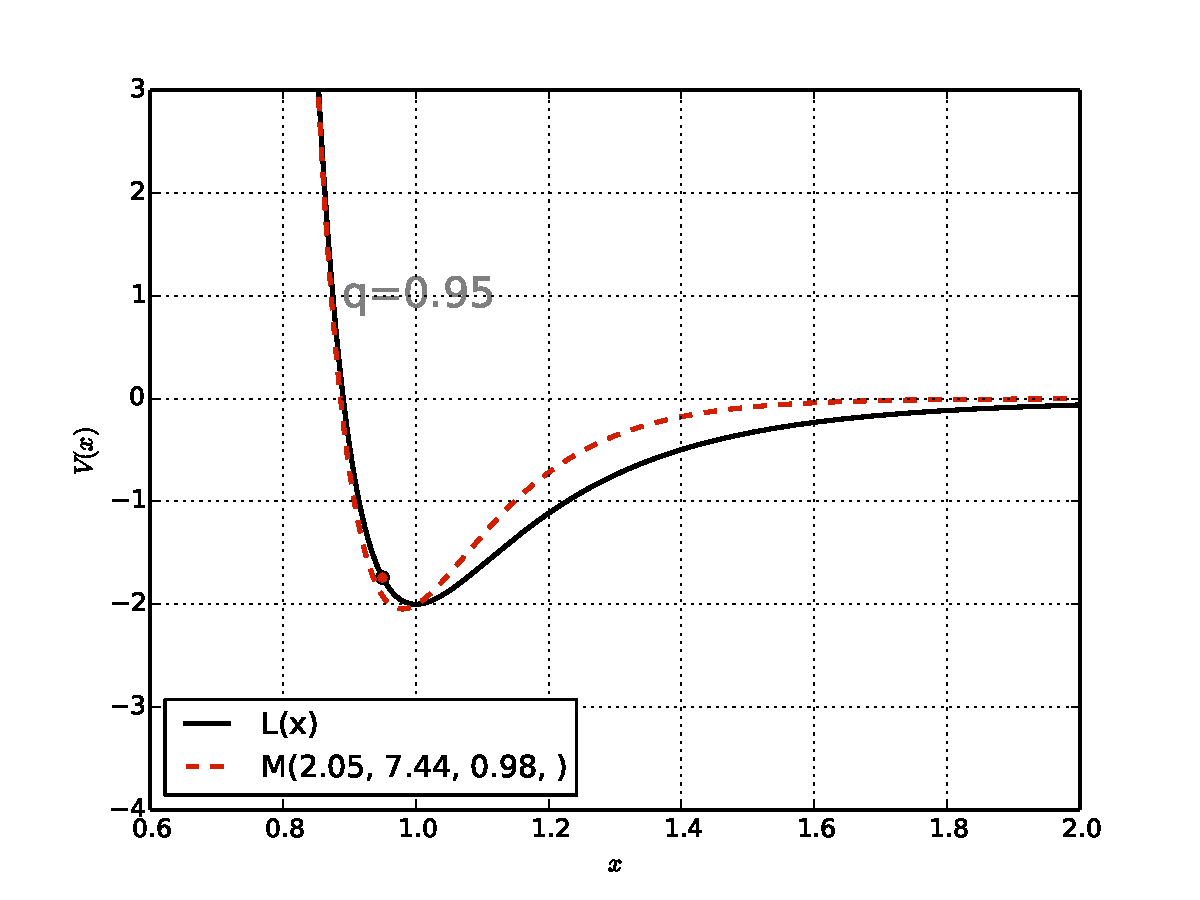
\includegraphics[width=0.5\linewidth]{./figures/MorseFitsCurvefit/curvefit095.pdf}
%    }\\
%    \subfloat[][]{
%	\label{fig:CurveFit0975}
%	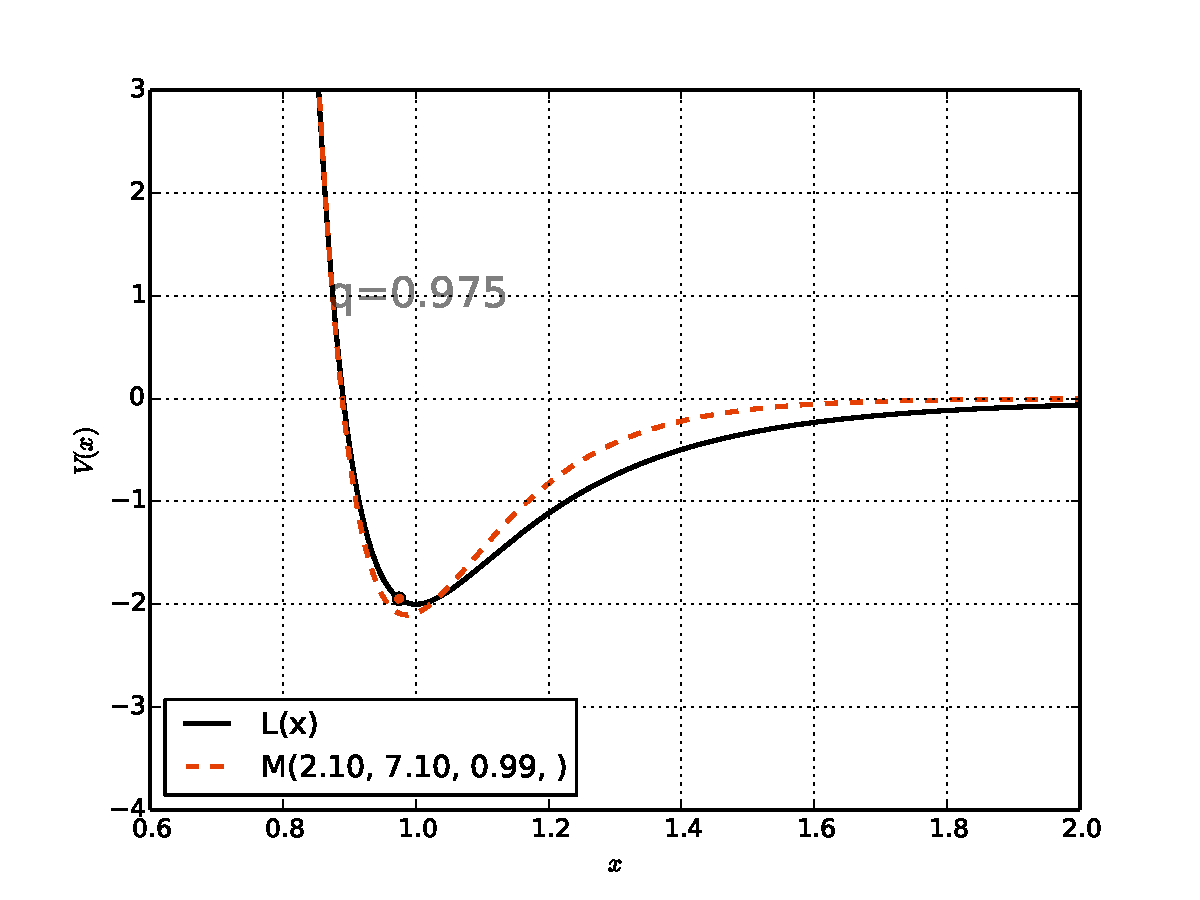
\includegraphics[width=0.5\linewidth]{./figures/MorseFitsCurvefit/curvefit0975.pdf}
%    }
%    \subfloat[][]{
%	\label{fig:CurveFit10}
%	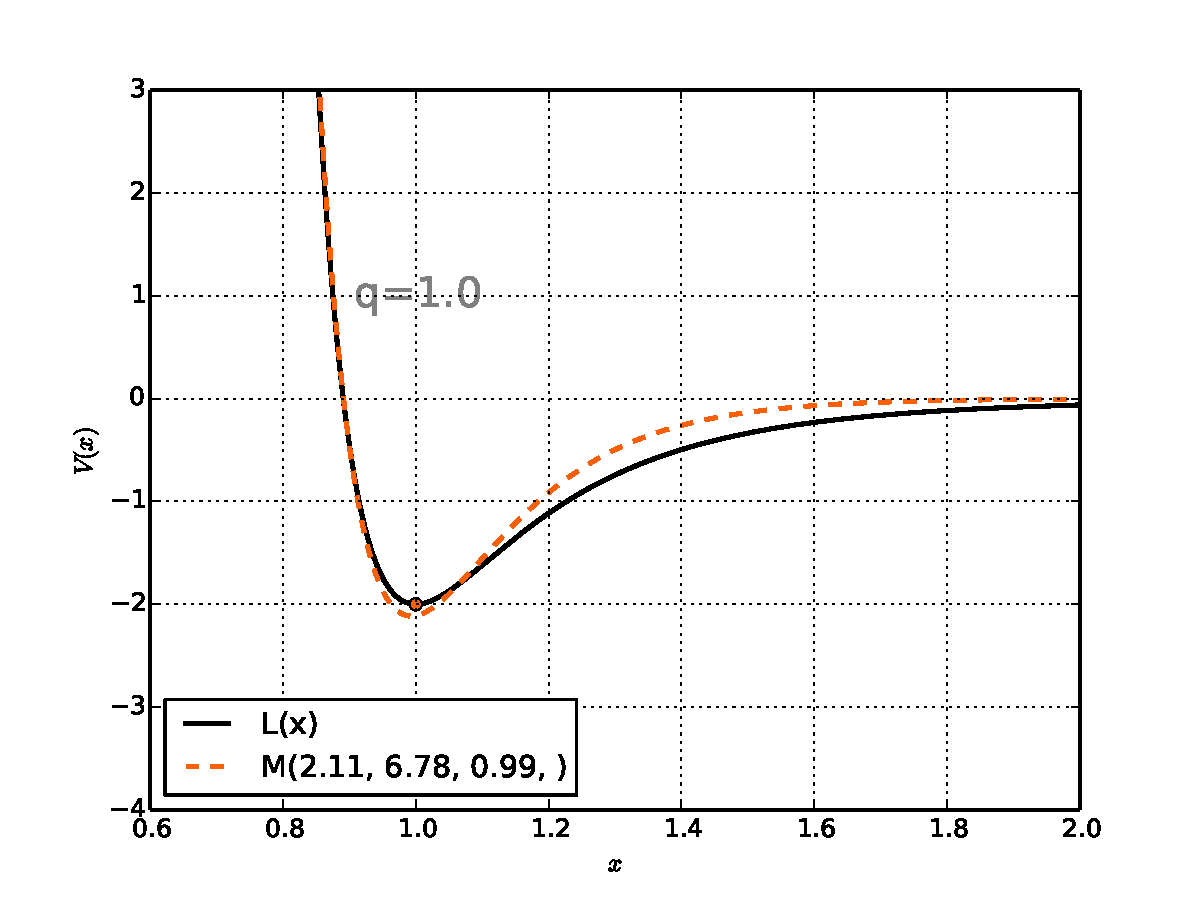
\includegraphics[width=0.5\linewidth]{./figures/MorseFitsCurvefit/curvefit10.pdf}
%    }
%    \\
%     \subfloat[][]{
%	\label{fig:CurveFit11}
%	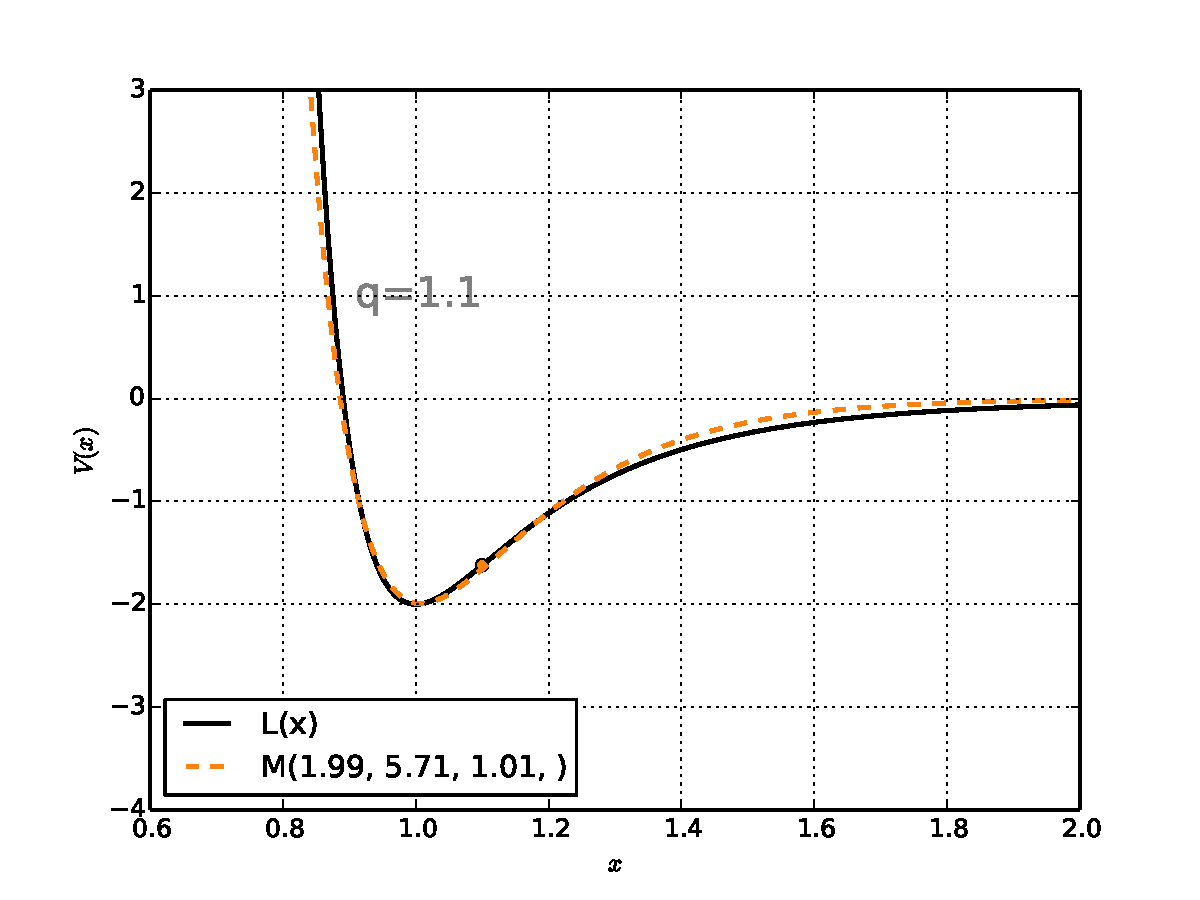
\includegraphics[width=0.5\linewidth]{./figures/MorseFitsCurvefit/curvefit11.pdf}
%    }
%    \subfloat[][]{
%	\label{fig:CurveFit115}
%	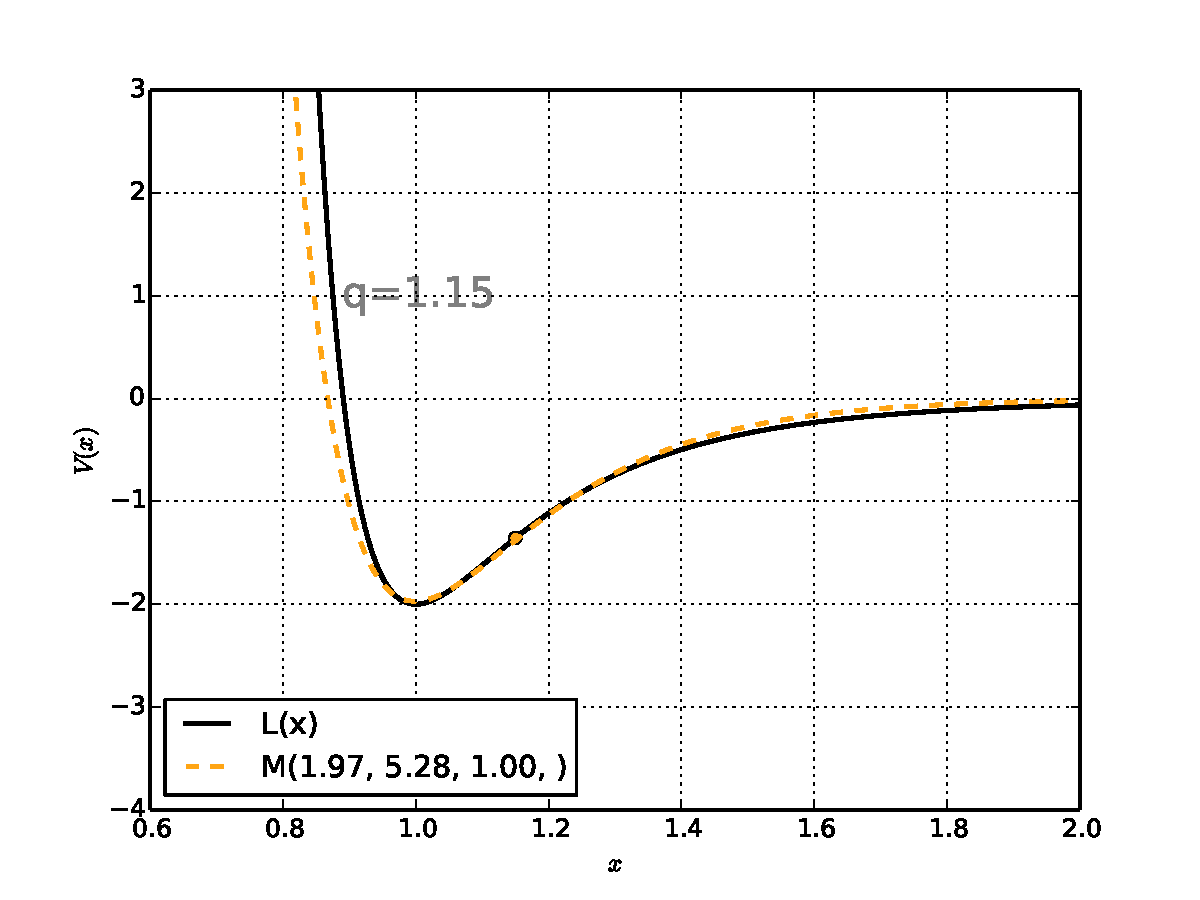
\includegraphics[width=0.5\linewidth]{./figures/MorseFitsCurvefit/curvefit115.pdf}
%    }\\
%    \subfloat[][]{
%	\label{fig:CurveFit12}
%	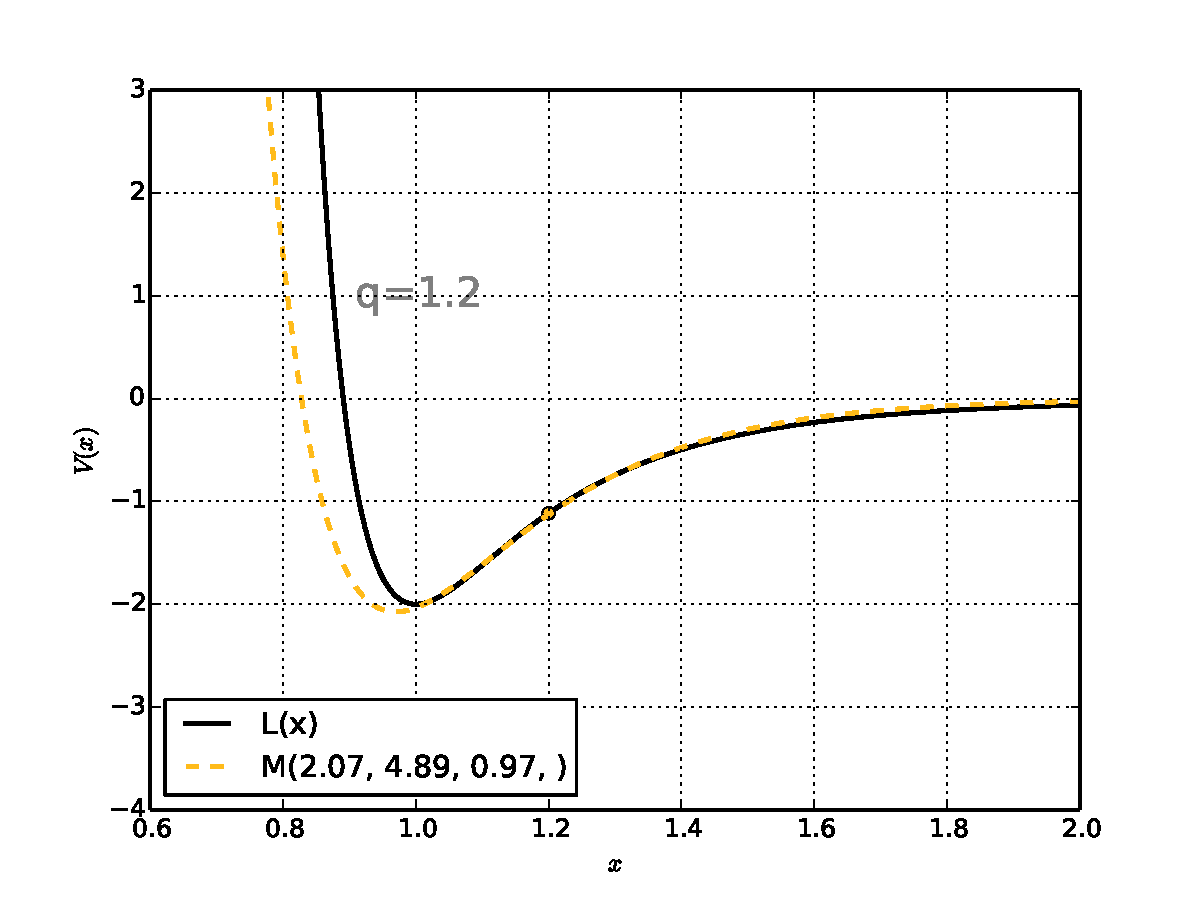
\includegraphics[width=0.5\linewidth]{./figures/MorseFitsCurvefit/curvefit12.pdf}
%    }
%    \subfloat[][]{
%	\label{fig:CurveFit125}
%	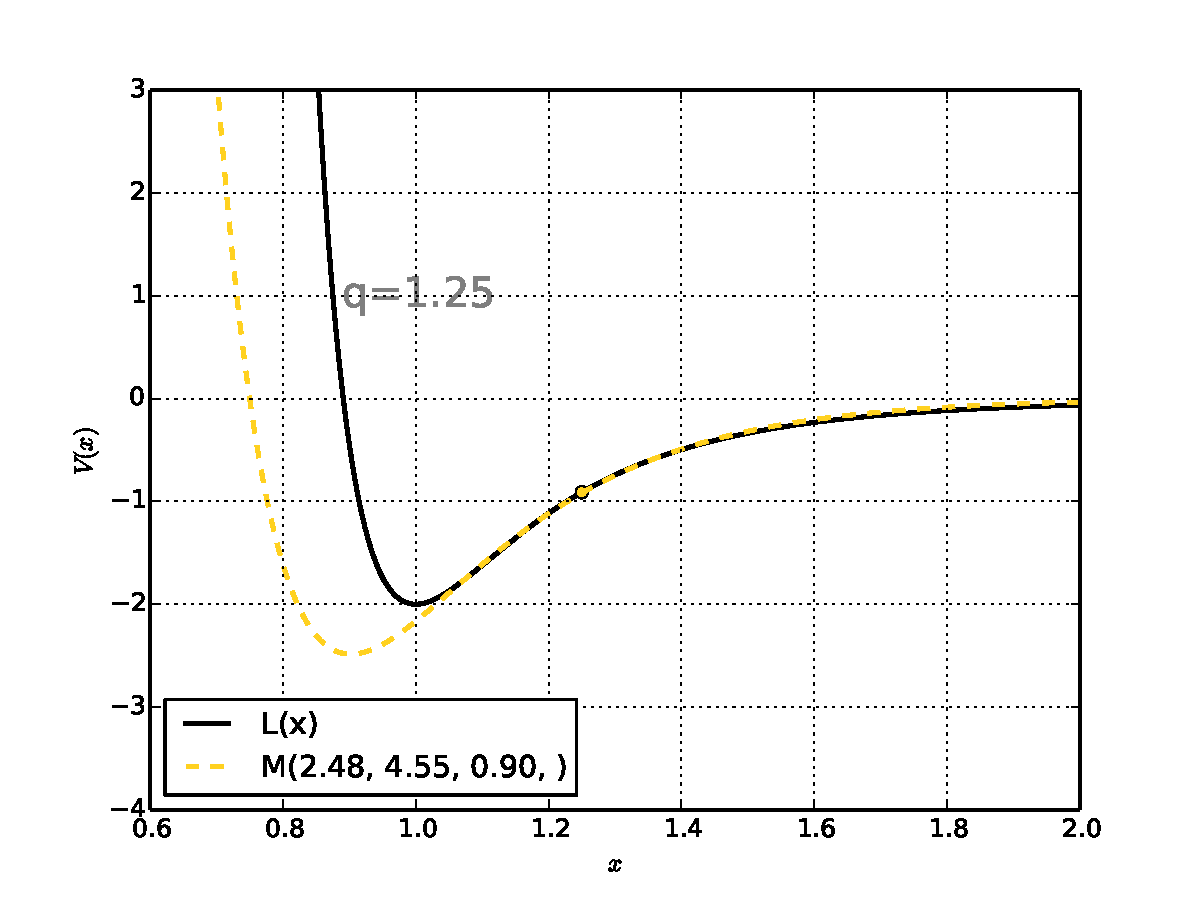
\includegraphics[width=0.5\linewidth]{./figures/MorseFitsCurvefit/curvefit125.pdf}
%    }
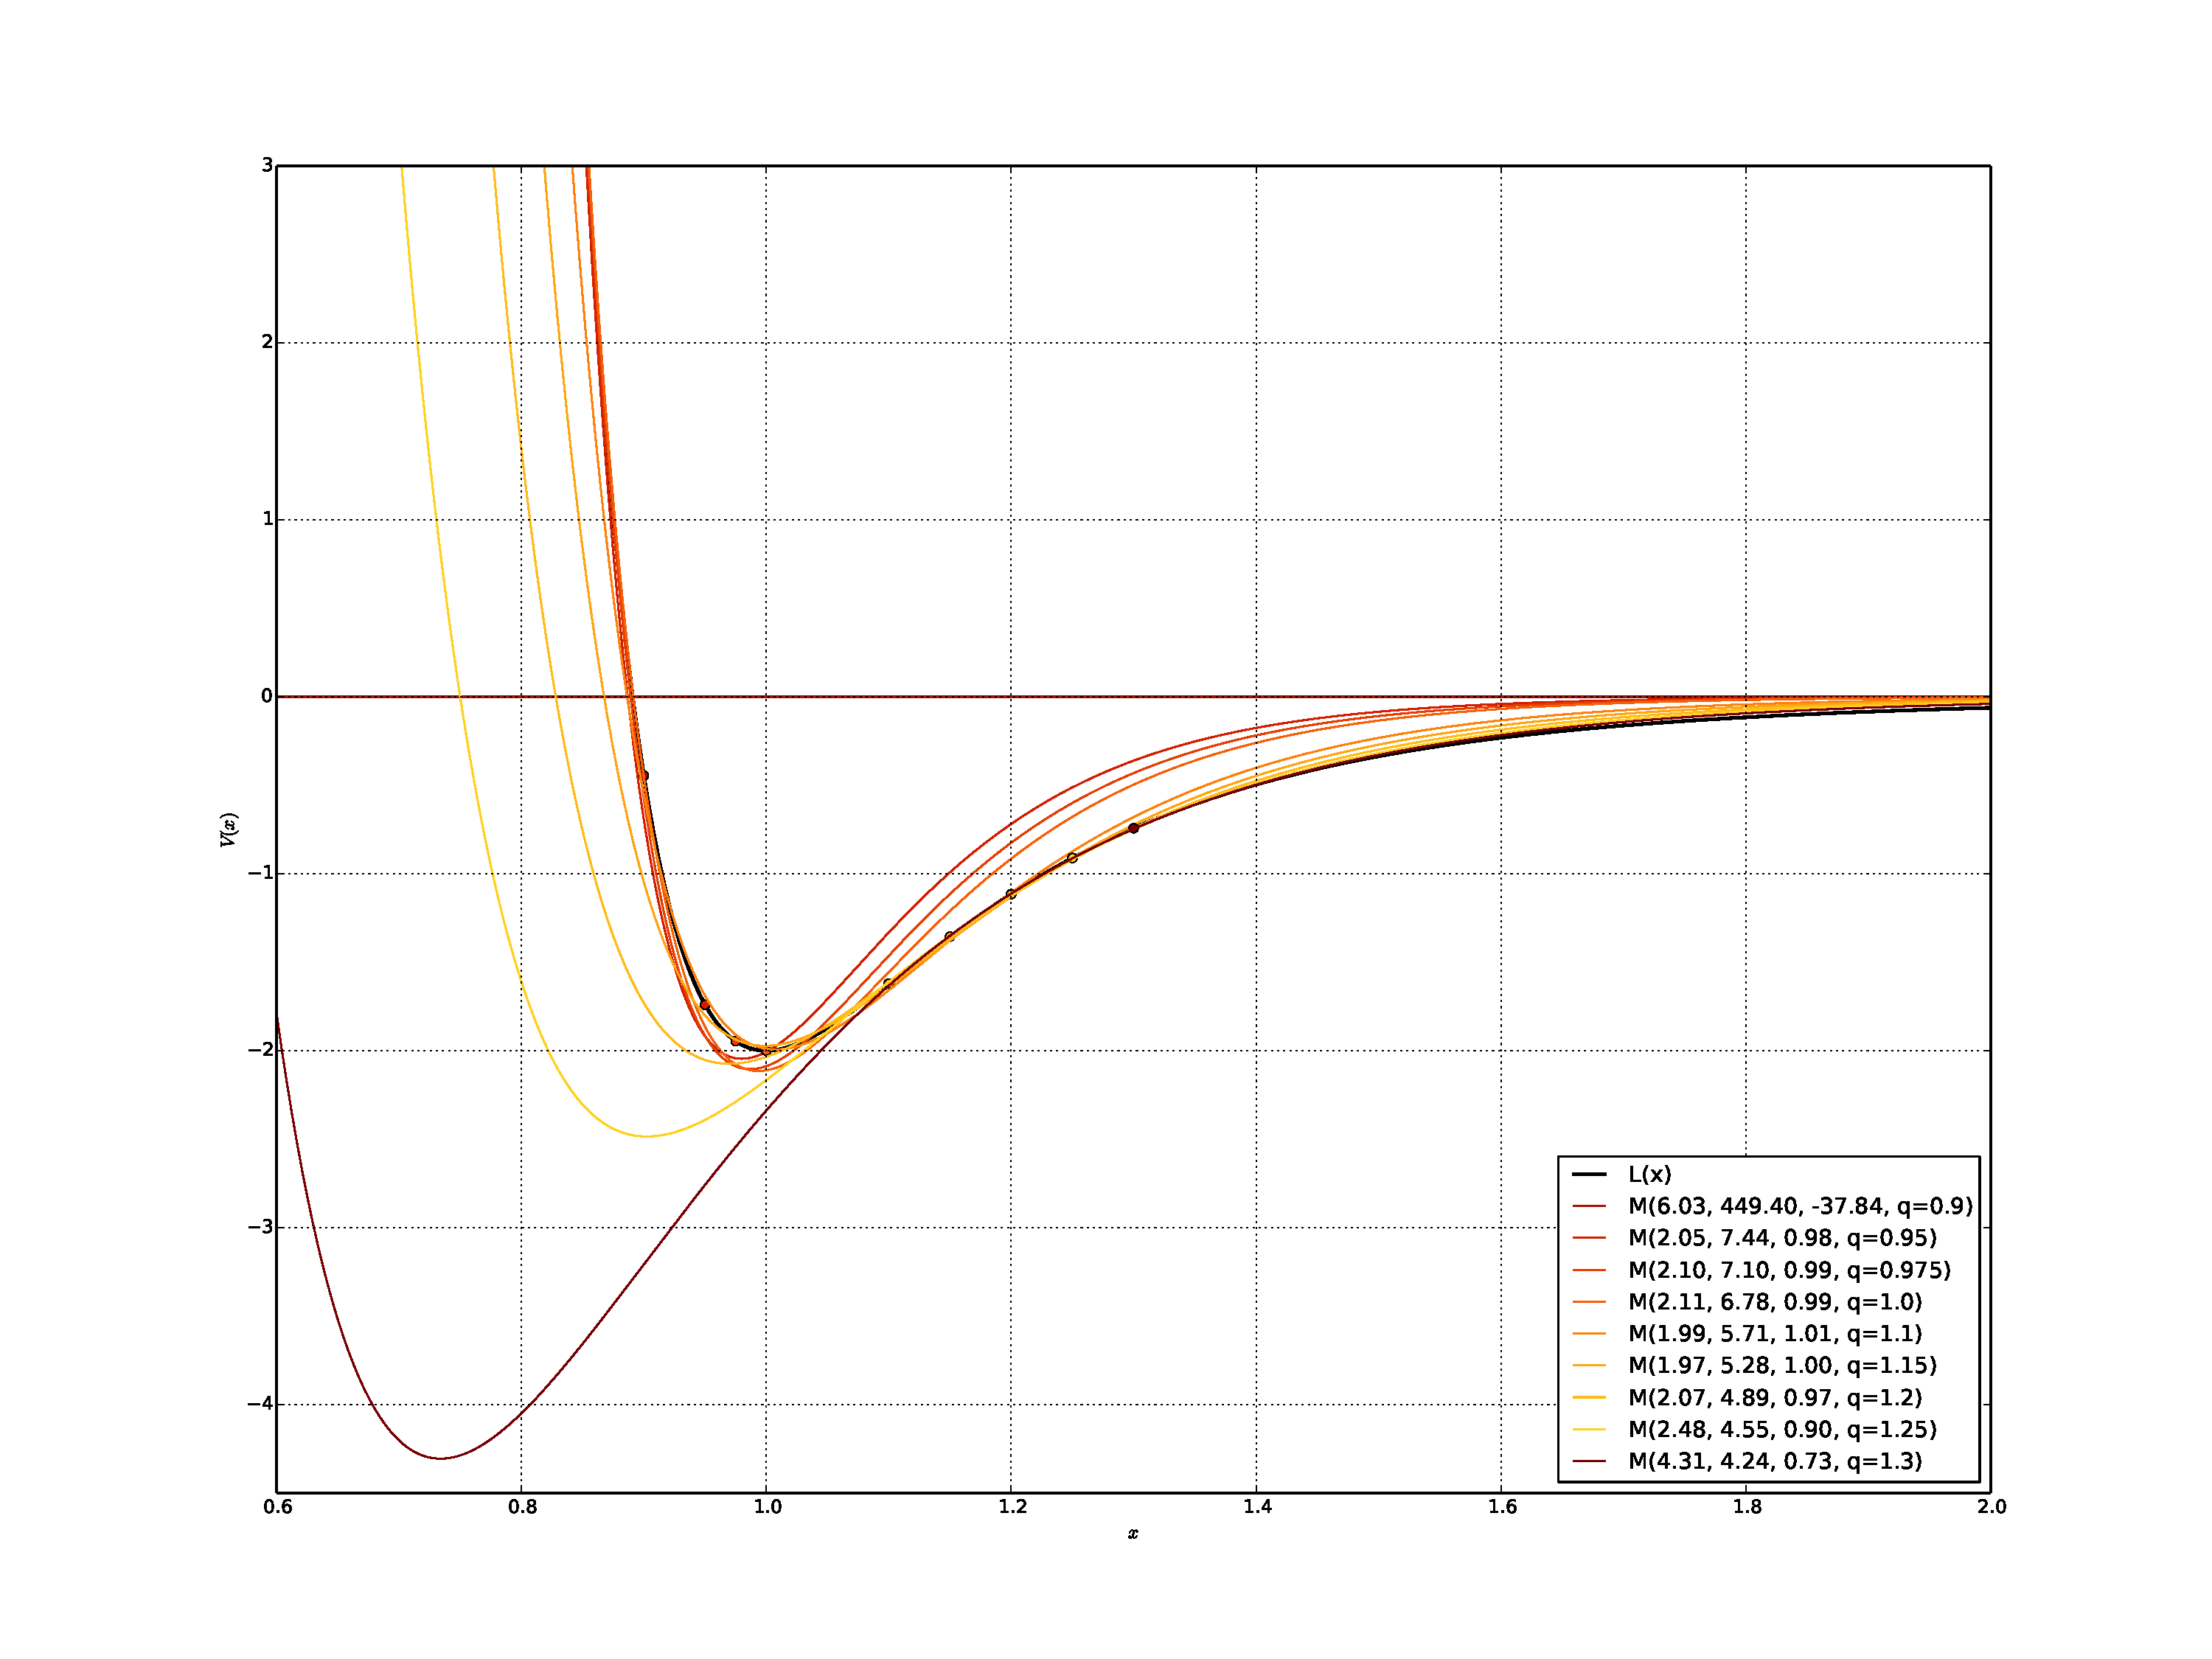
\includegraphics[width=1.2\linewidth]{./figures/MorseFitsCurvefit/curvefitAll.pdf}
    \\
%	\subfloat[][]{
%	\label{fig:CurveFit13}
%	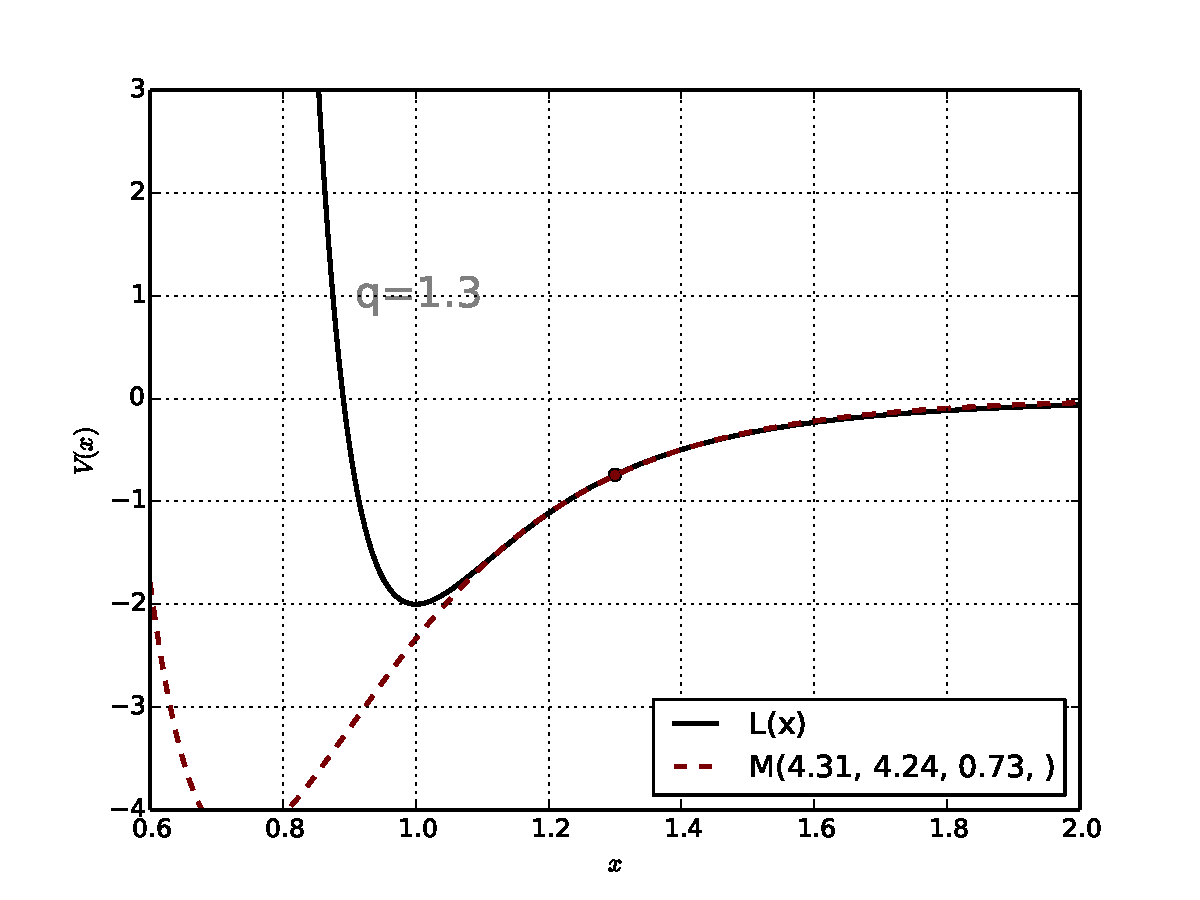
\includegraphics[width=0.5\linewidth]{./figures/MorseFitsCurvefit/curvefit13.pdf}
%    }
       \caption[\texttt{curve\_fit} fits to the Morse potential]{
	\texttt{curve\_fit} fits to the Morse potential
    \label{fig:MorseFitsCurvefit}
    }

\end{figure}



%\begin{figure}[h!]
%	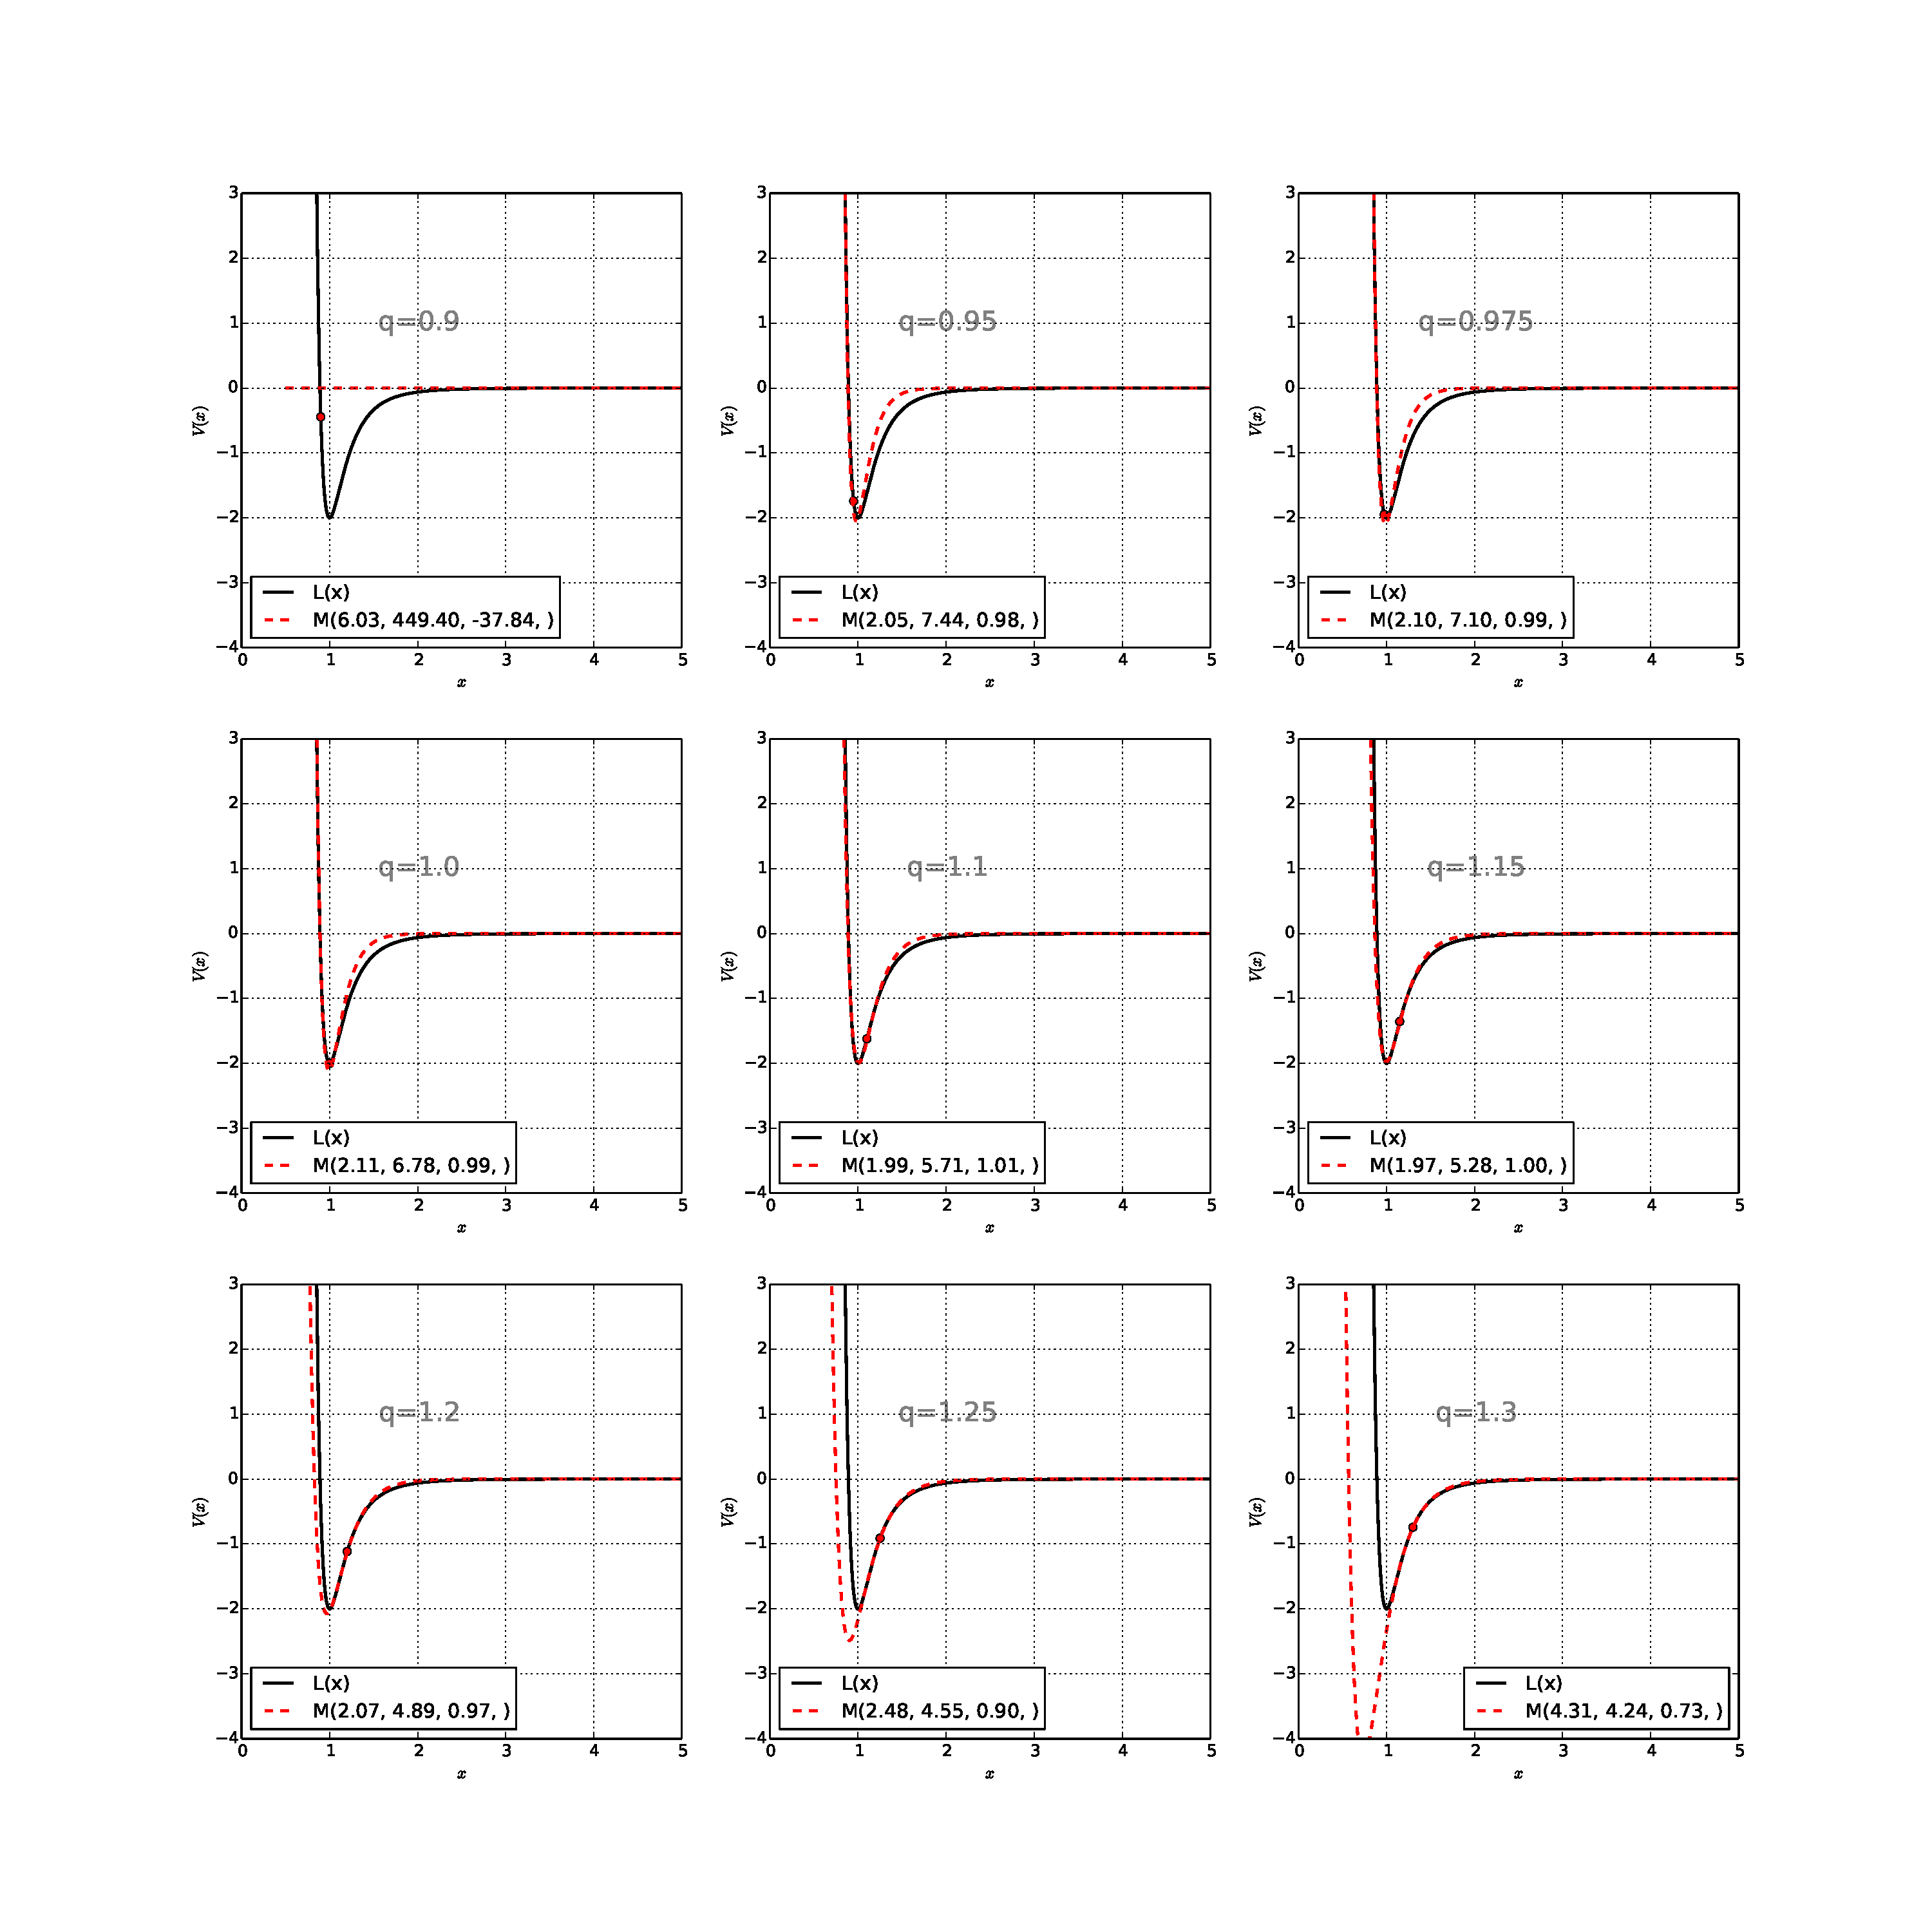
\includegraphics[width=1.0\linewidth]{./figures/MorseFitsCurvefit/fits_curvefit.pdf}
%	\caption[\texttt{curve\_fit} fits to the Morse potential]{
%	
%	    \label{fig:MorseFitsCurvefit}
%	}
%
%\end{figure}




% subsection curve_fit (end)

\subsection{\texttt{leastsq}}% (fold)
\label{subsec:leastsq}
As already said, the only difference to the previous algorithm is that we also provide an analytical Jacobian,
in our case given by
\begin{align}
    J_i=J(x_i)+
    \begin{pmatrix}
    	e^{-2\beta(x_i-x_0)}-2e^{-\beta(x_i-x_0)}\\
	-2 V_0 (x_i-x_0)(e^{-2\beta(x_i-x_0)}-2e^{-\beta(x_i-x_0)})\\
	2\beta(e^{\beta(x_i-x_0)}-2e^{-\beta(x_i-x_0)}
    \end{pmatrix}
\end{align}
% subsection leastsq (end)

\begin{figure}[h!]
    \centering
%     \subfloat[][]{
%	\label{fig:LeastSq09}
%	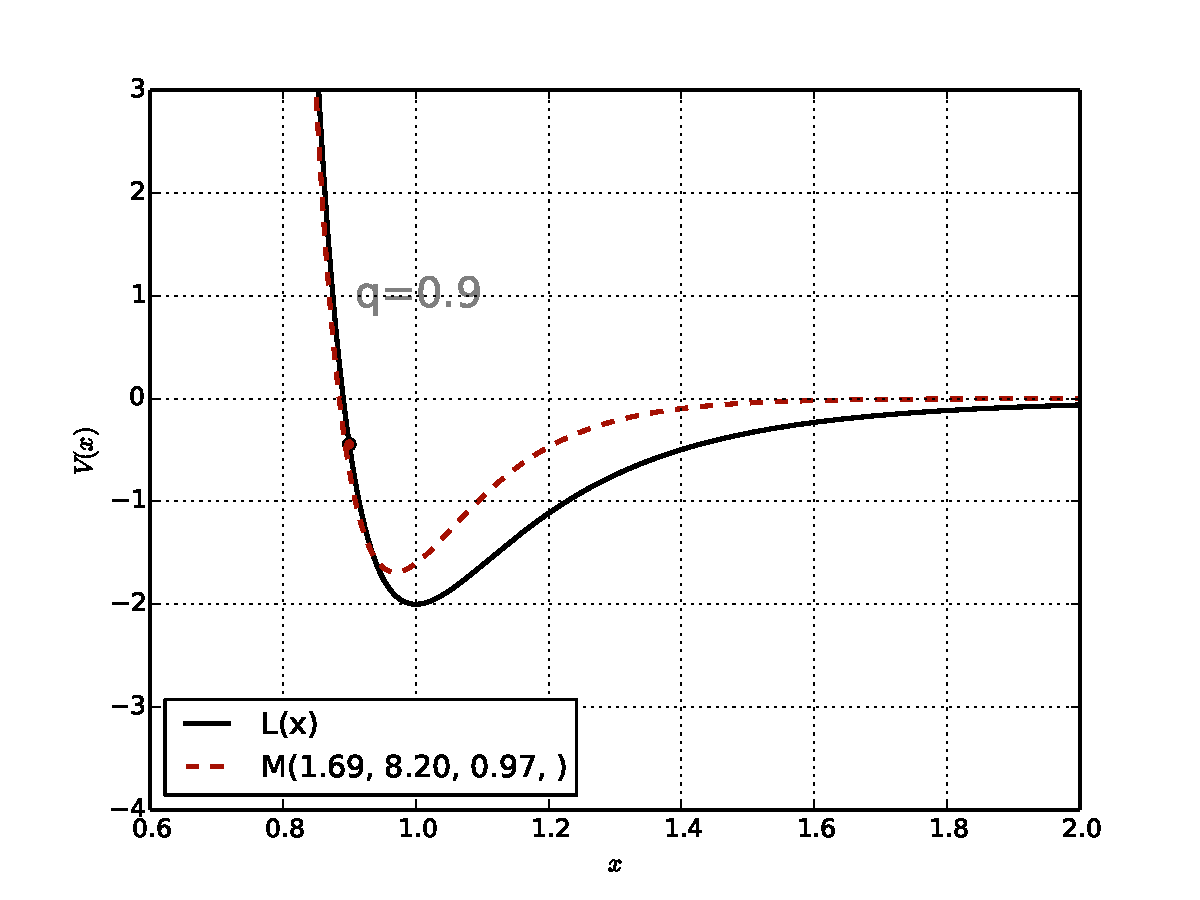
\includegraphics[width=0.5\linewidth]{./figures/MorseFitsLeastsq/leastsq09.pdf}
%    }
%    \subfloat[][]{
%	\label{fig:LeastSq095}
%	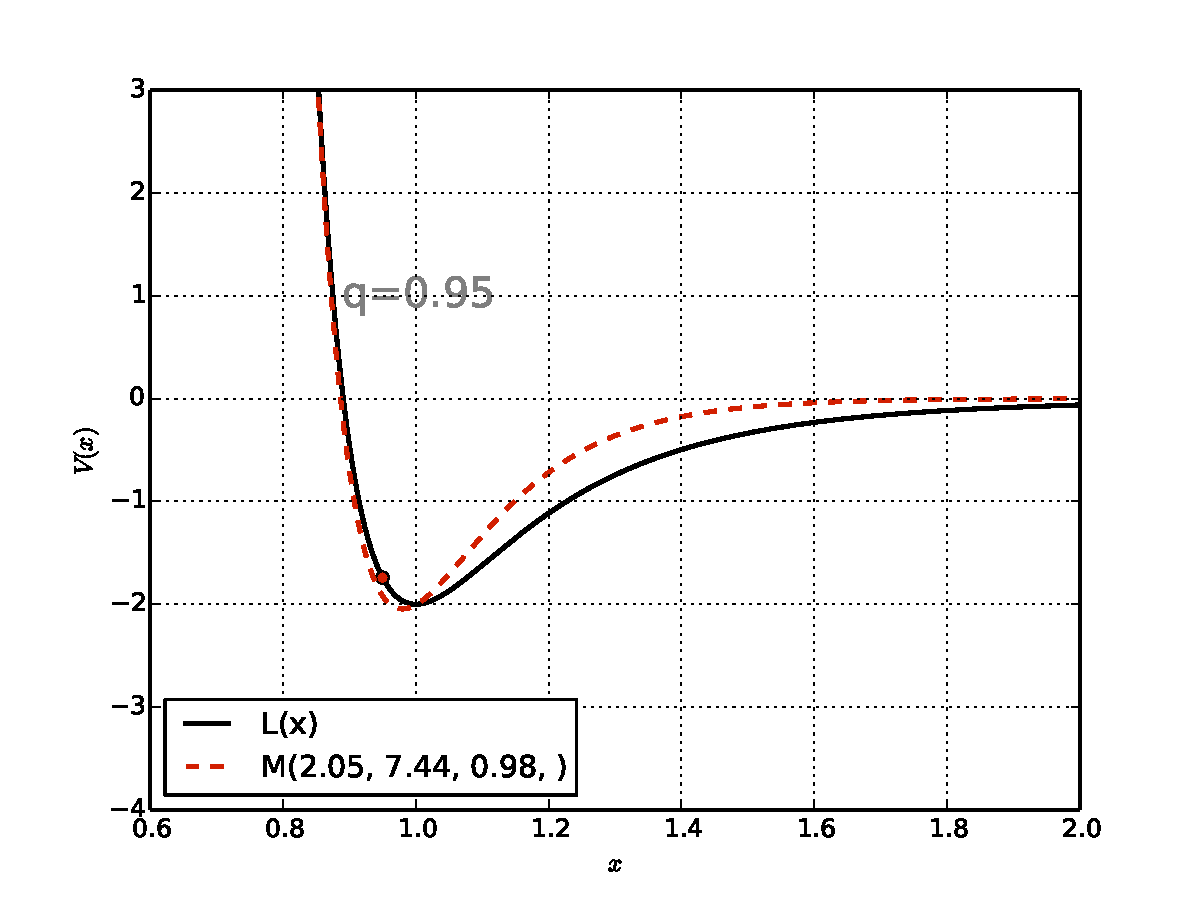
\includegraphics[width=0.5\linewidth]{./figures/MorseFitsLeastsq/leastsq095.pdf}
%    }\\
%    \subfloat[][]{
%	\label{fig:LeastSq0975}
%	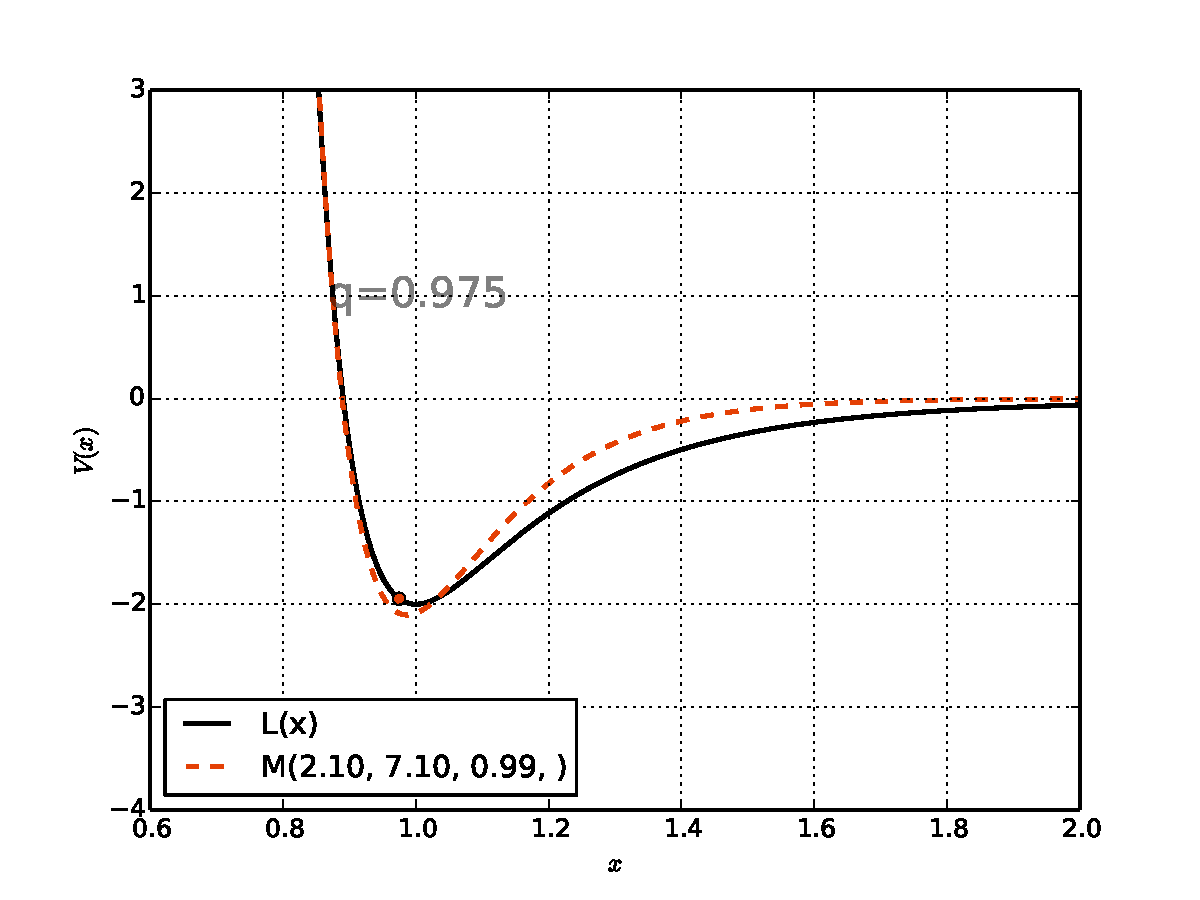
\includegraphics[width=0.5\linewidth]{./figures/MorseFitsLeastsq/leastsq0975.pdf}
%    }
%    \subfloat[][]{
%	\label{fig:LeastSq10}
%	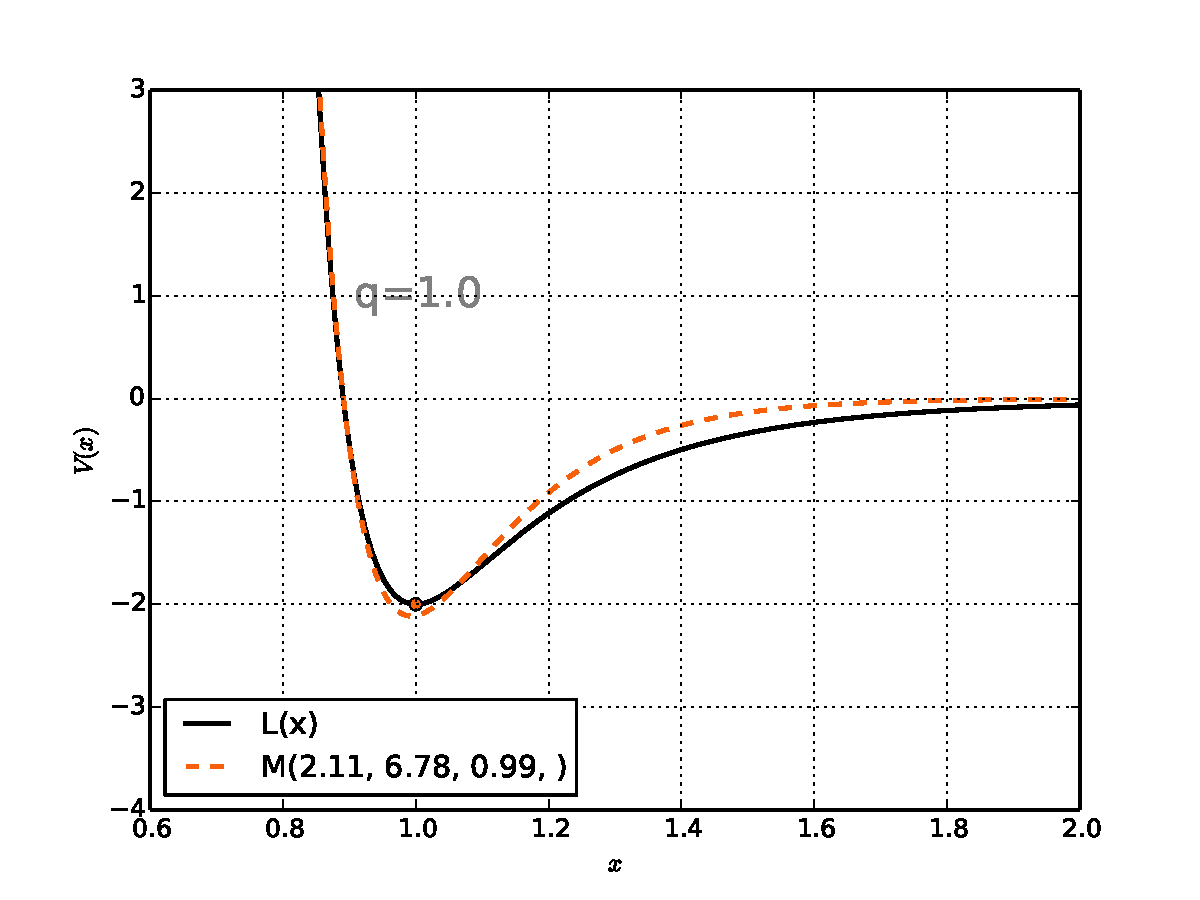
\includegraphics[width=0.5\linewidth]{./figures/MorseFitsLeastsq/leastsq10.pdf}
%    }
%    \\
%     \subfloat[][]{
%	\label{fig:LeastSq11}
%	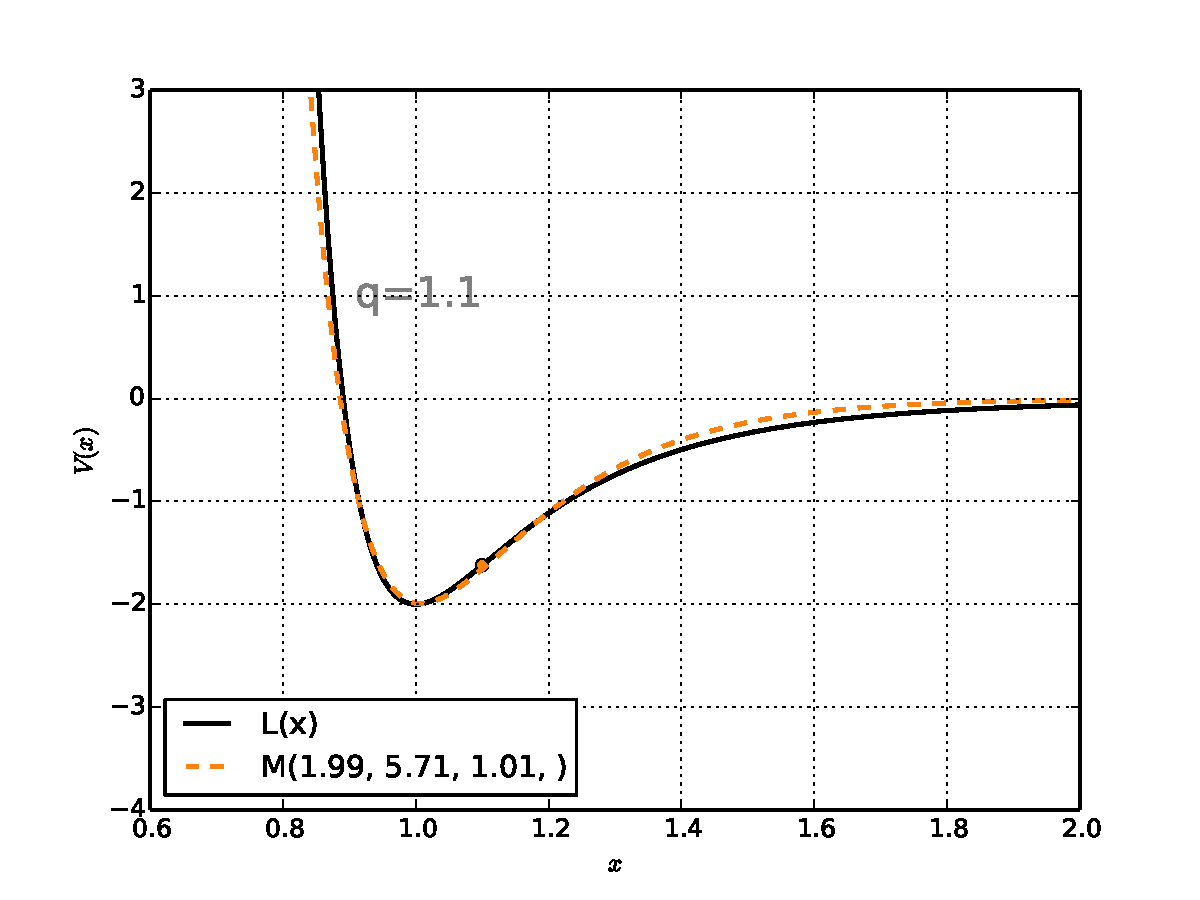
\includegraphics[width=0.5\linewidth]{./figures/MorseFitsLeastsq/leastsq11.pdf}
%    }
%    \subfloat[][]{
%	\label{fig:LeastSq115}
%	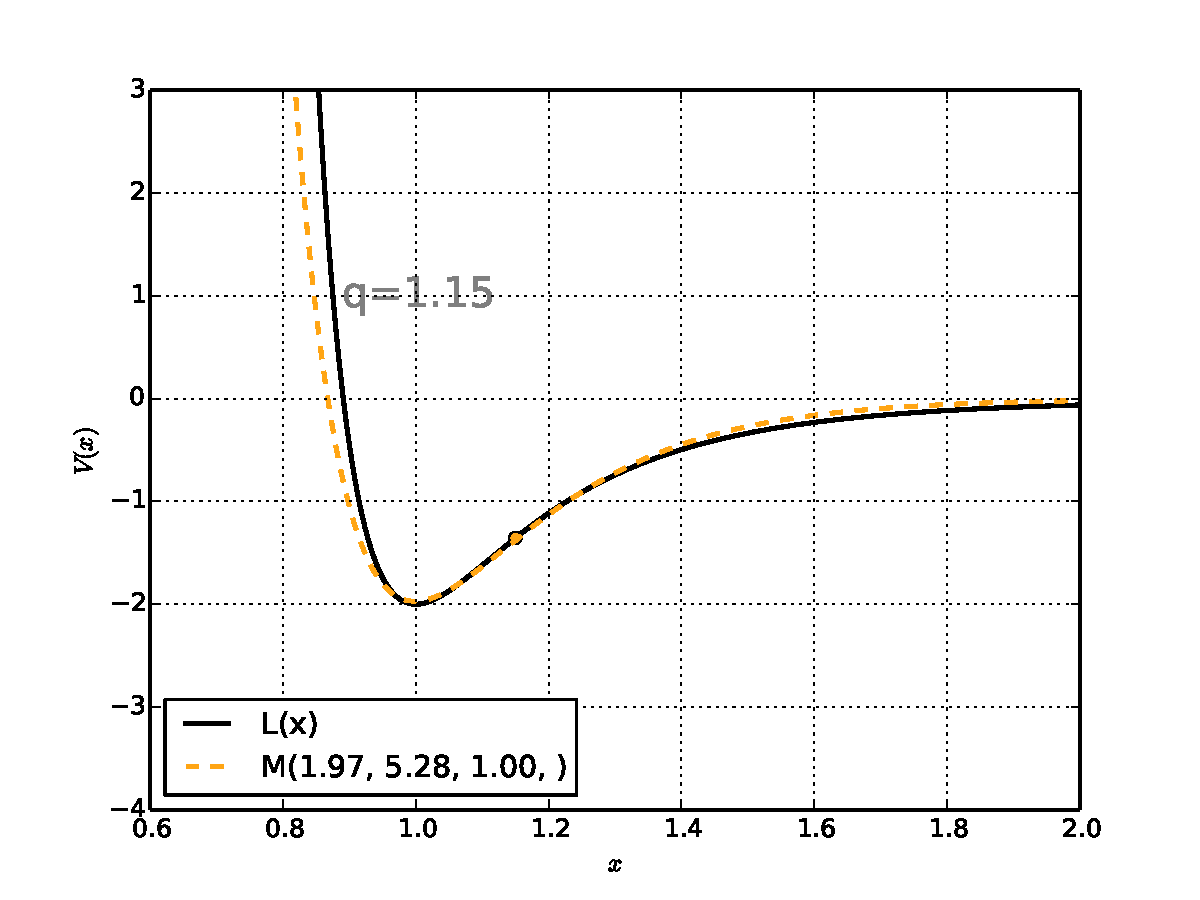
\includegraphics[width=0.5\linewidth]{./figures/MorseFitsLeastsq/leastsq115.pdf}
%    }\\
%    \subfloat[][]{
%	\label{fig:LeastSq12}
%	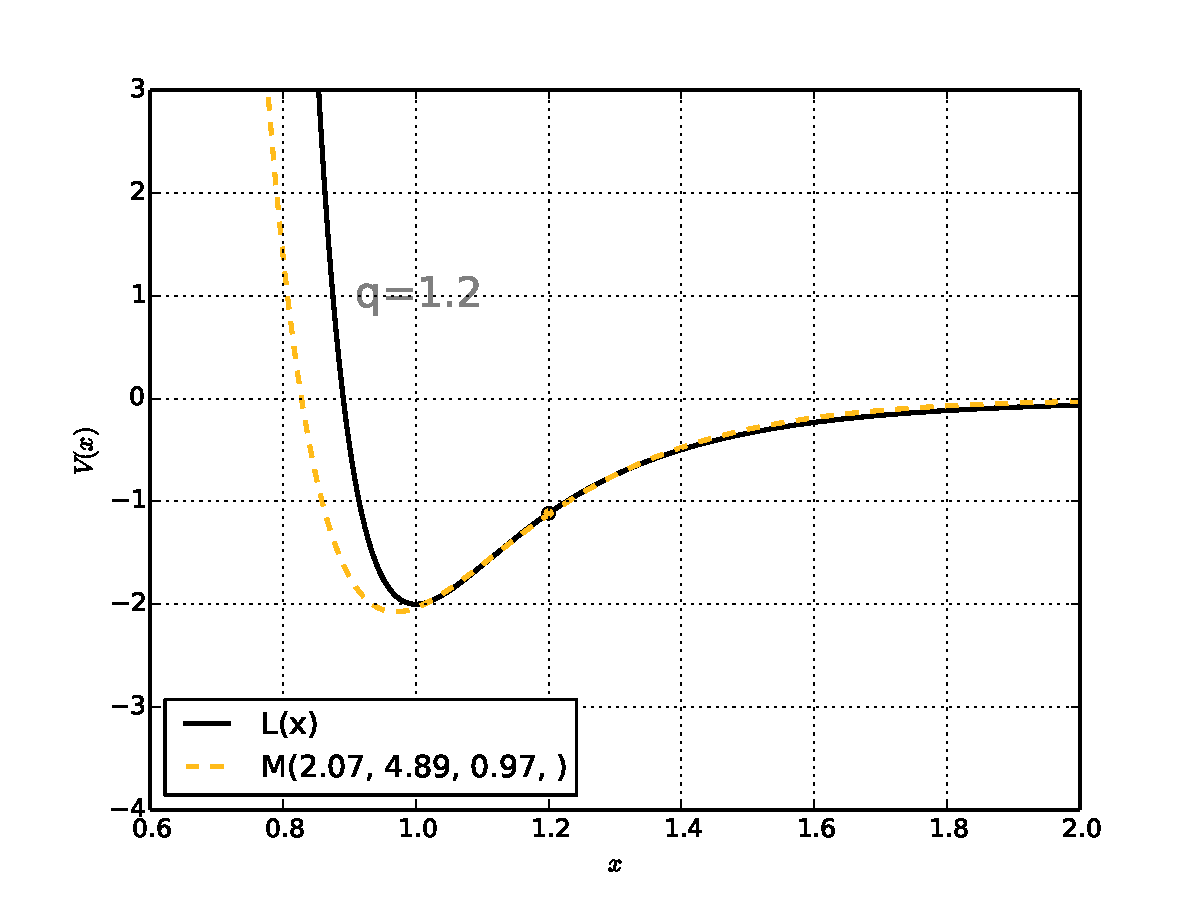
\includegraphics[width=0.5\linewidth]{./figures/MorseFitsLeastsq/leastsq12.pdf}
%    }
%    \subfloat[][]{
%	\label{fig:LeastSq125}
%	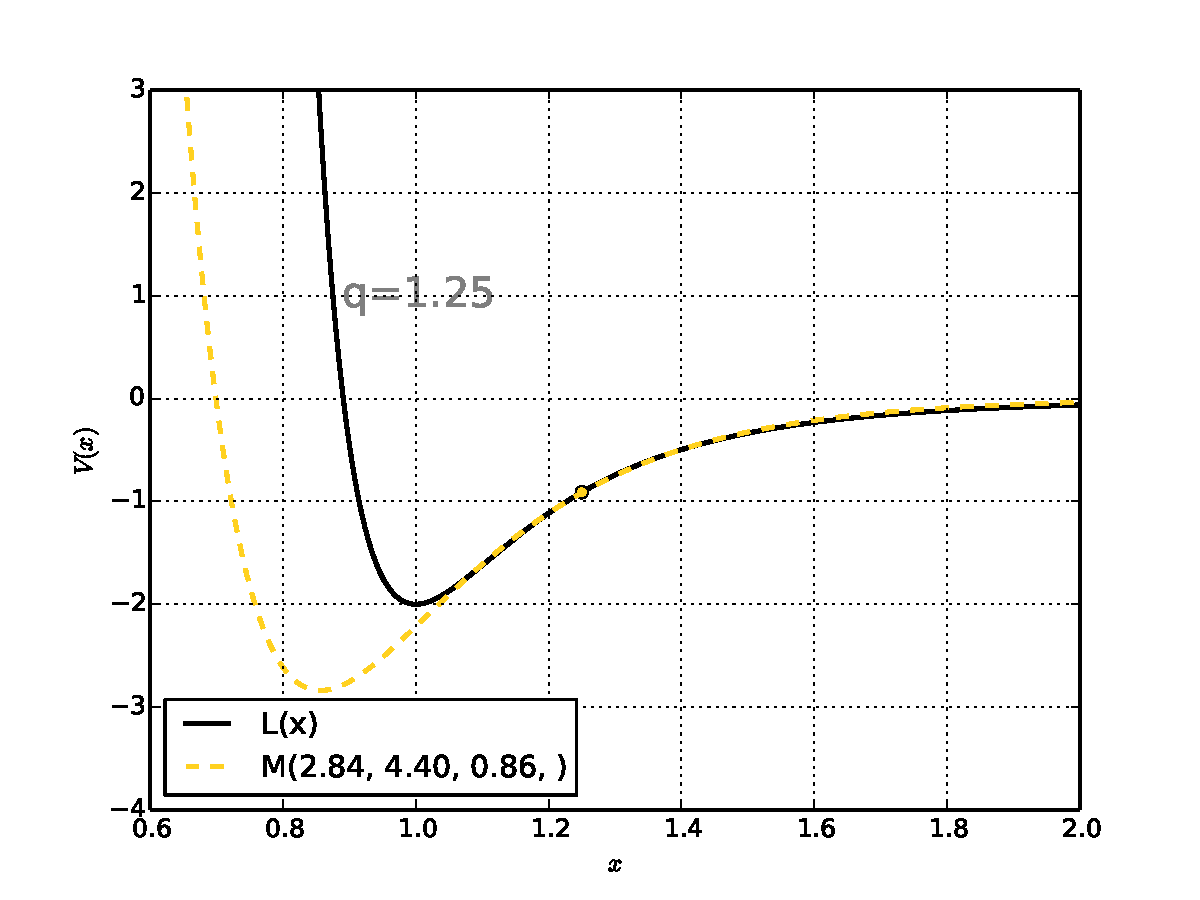
\includegraphics[width=0.5\linewidth]{./figures/MorseFitsLeastsq/leastsq125.pdf}
%    }
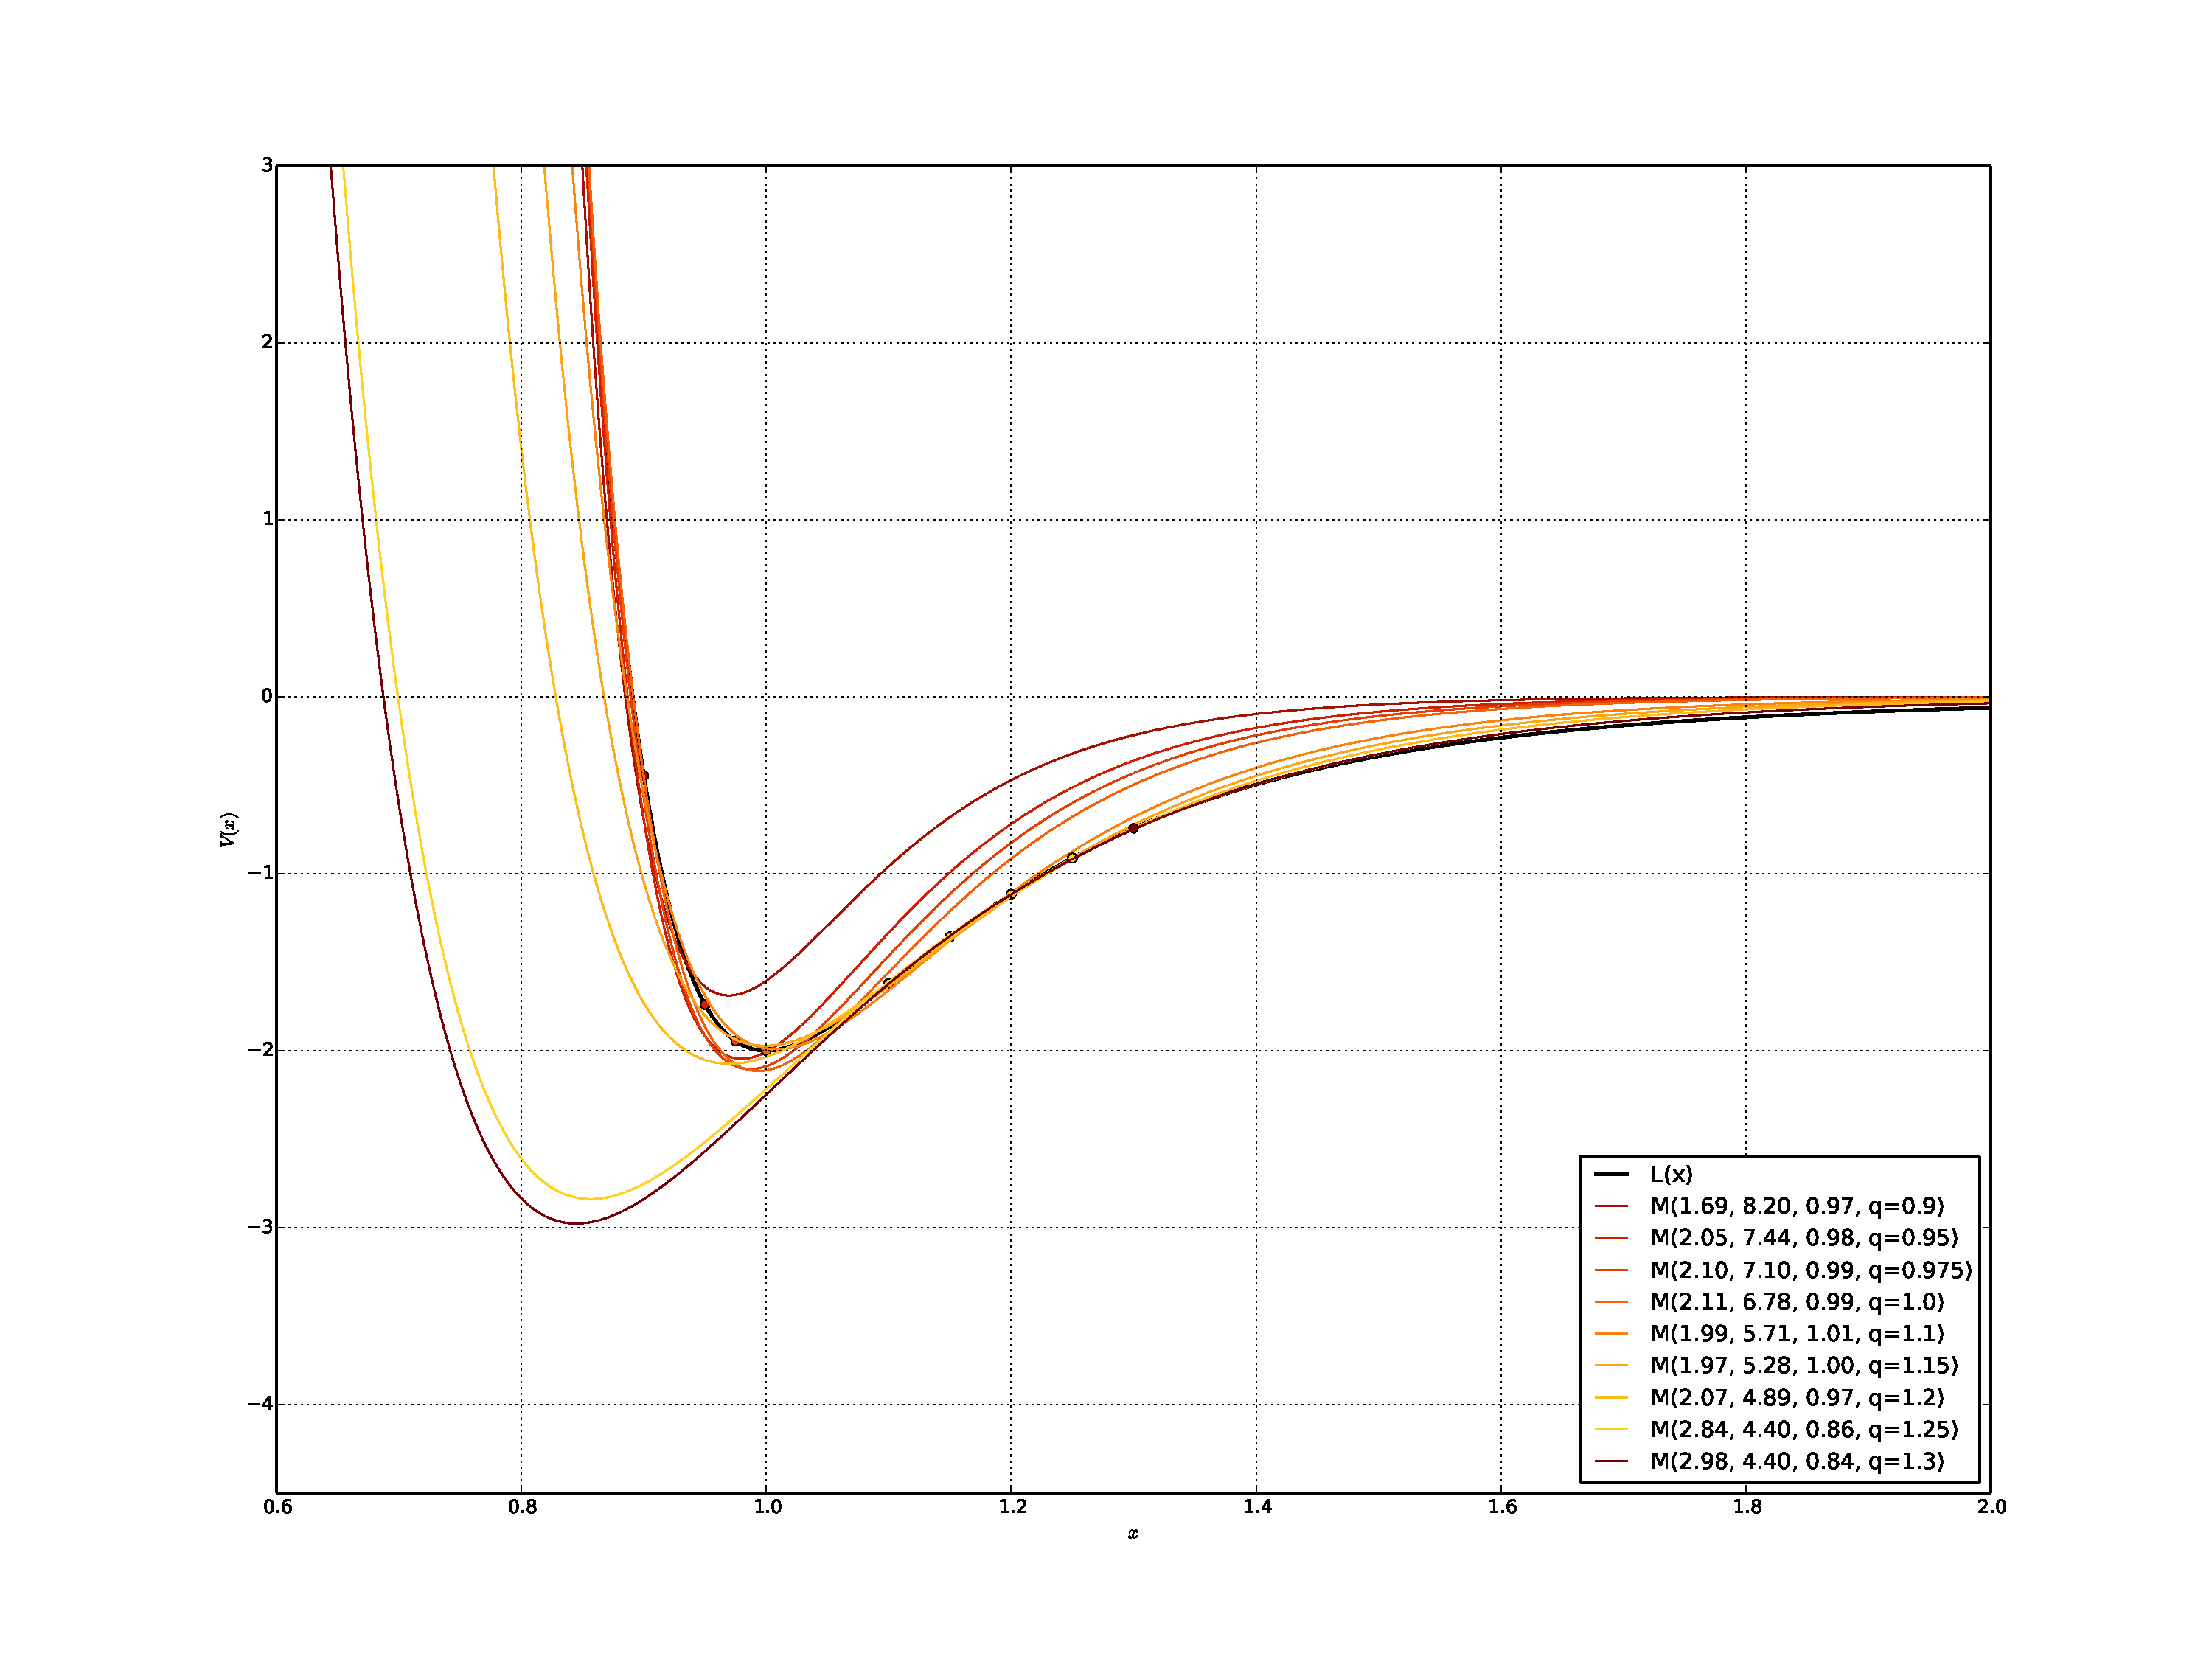
\includegraphics[width=1.2\linewidth]{./figures/MorseFitsLeastsq/leastsqAll.pdf}
    \\
%	\subfloat[][]{
%	\label{fig:LeastSq13}
%	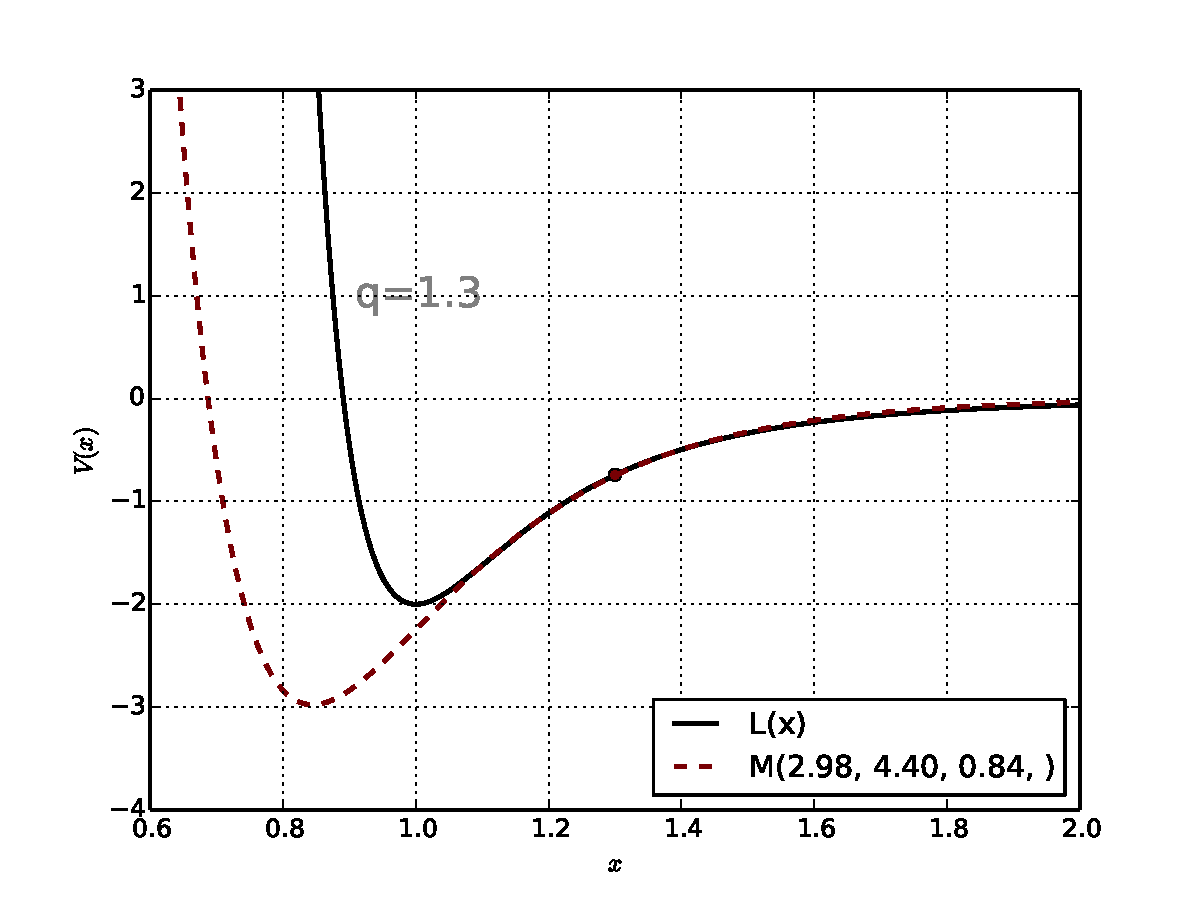
\includegraphics[width=0.5\linewidth]{./figures/MorseFitsLeastsq/leastsq13.pdf}
%    }

       \caption[\texttt{leastsq} fits to the Morse potential]{
	\texttt{leastsq} fits to the Morse potential
    \label{fig:MorseFitsLeastsq}
    }

\end{figure}


%\begin{figure}[h!]
%	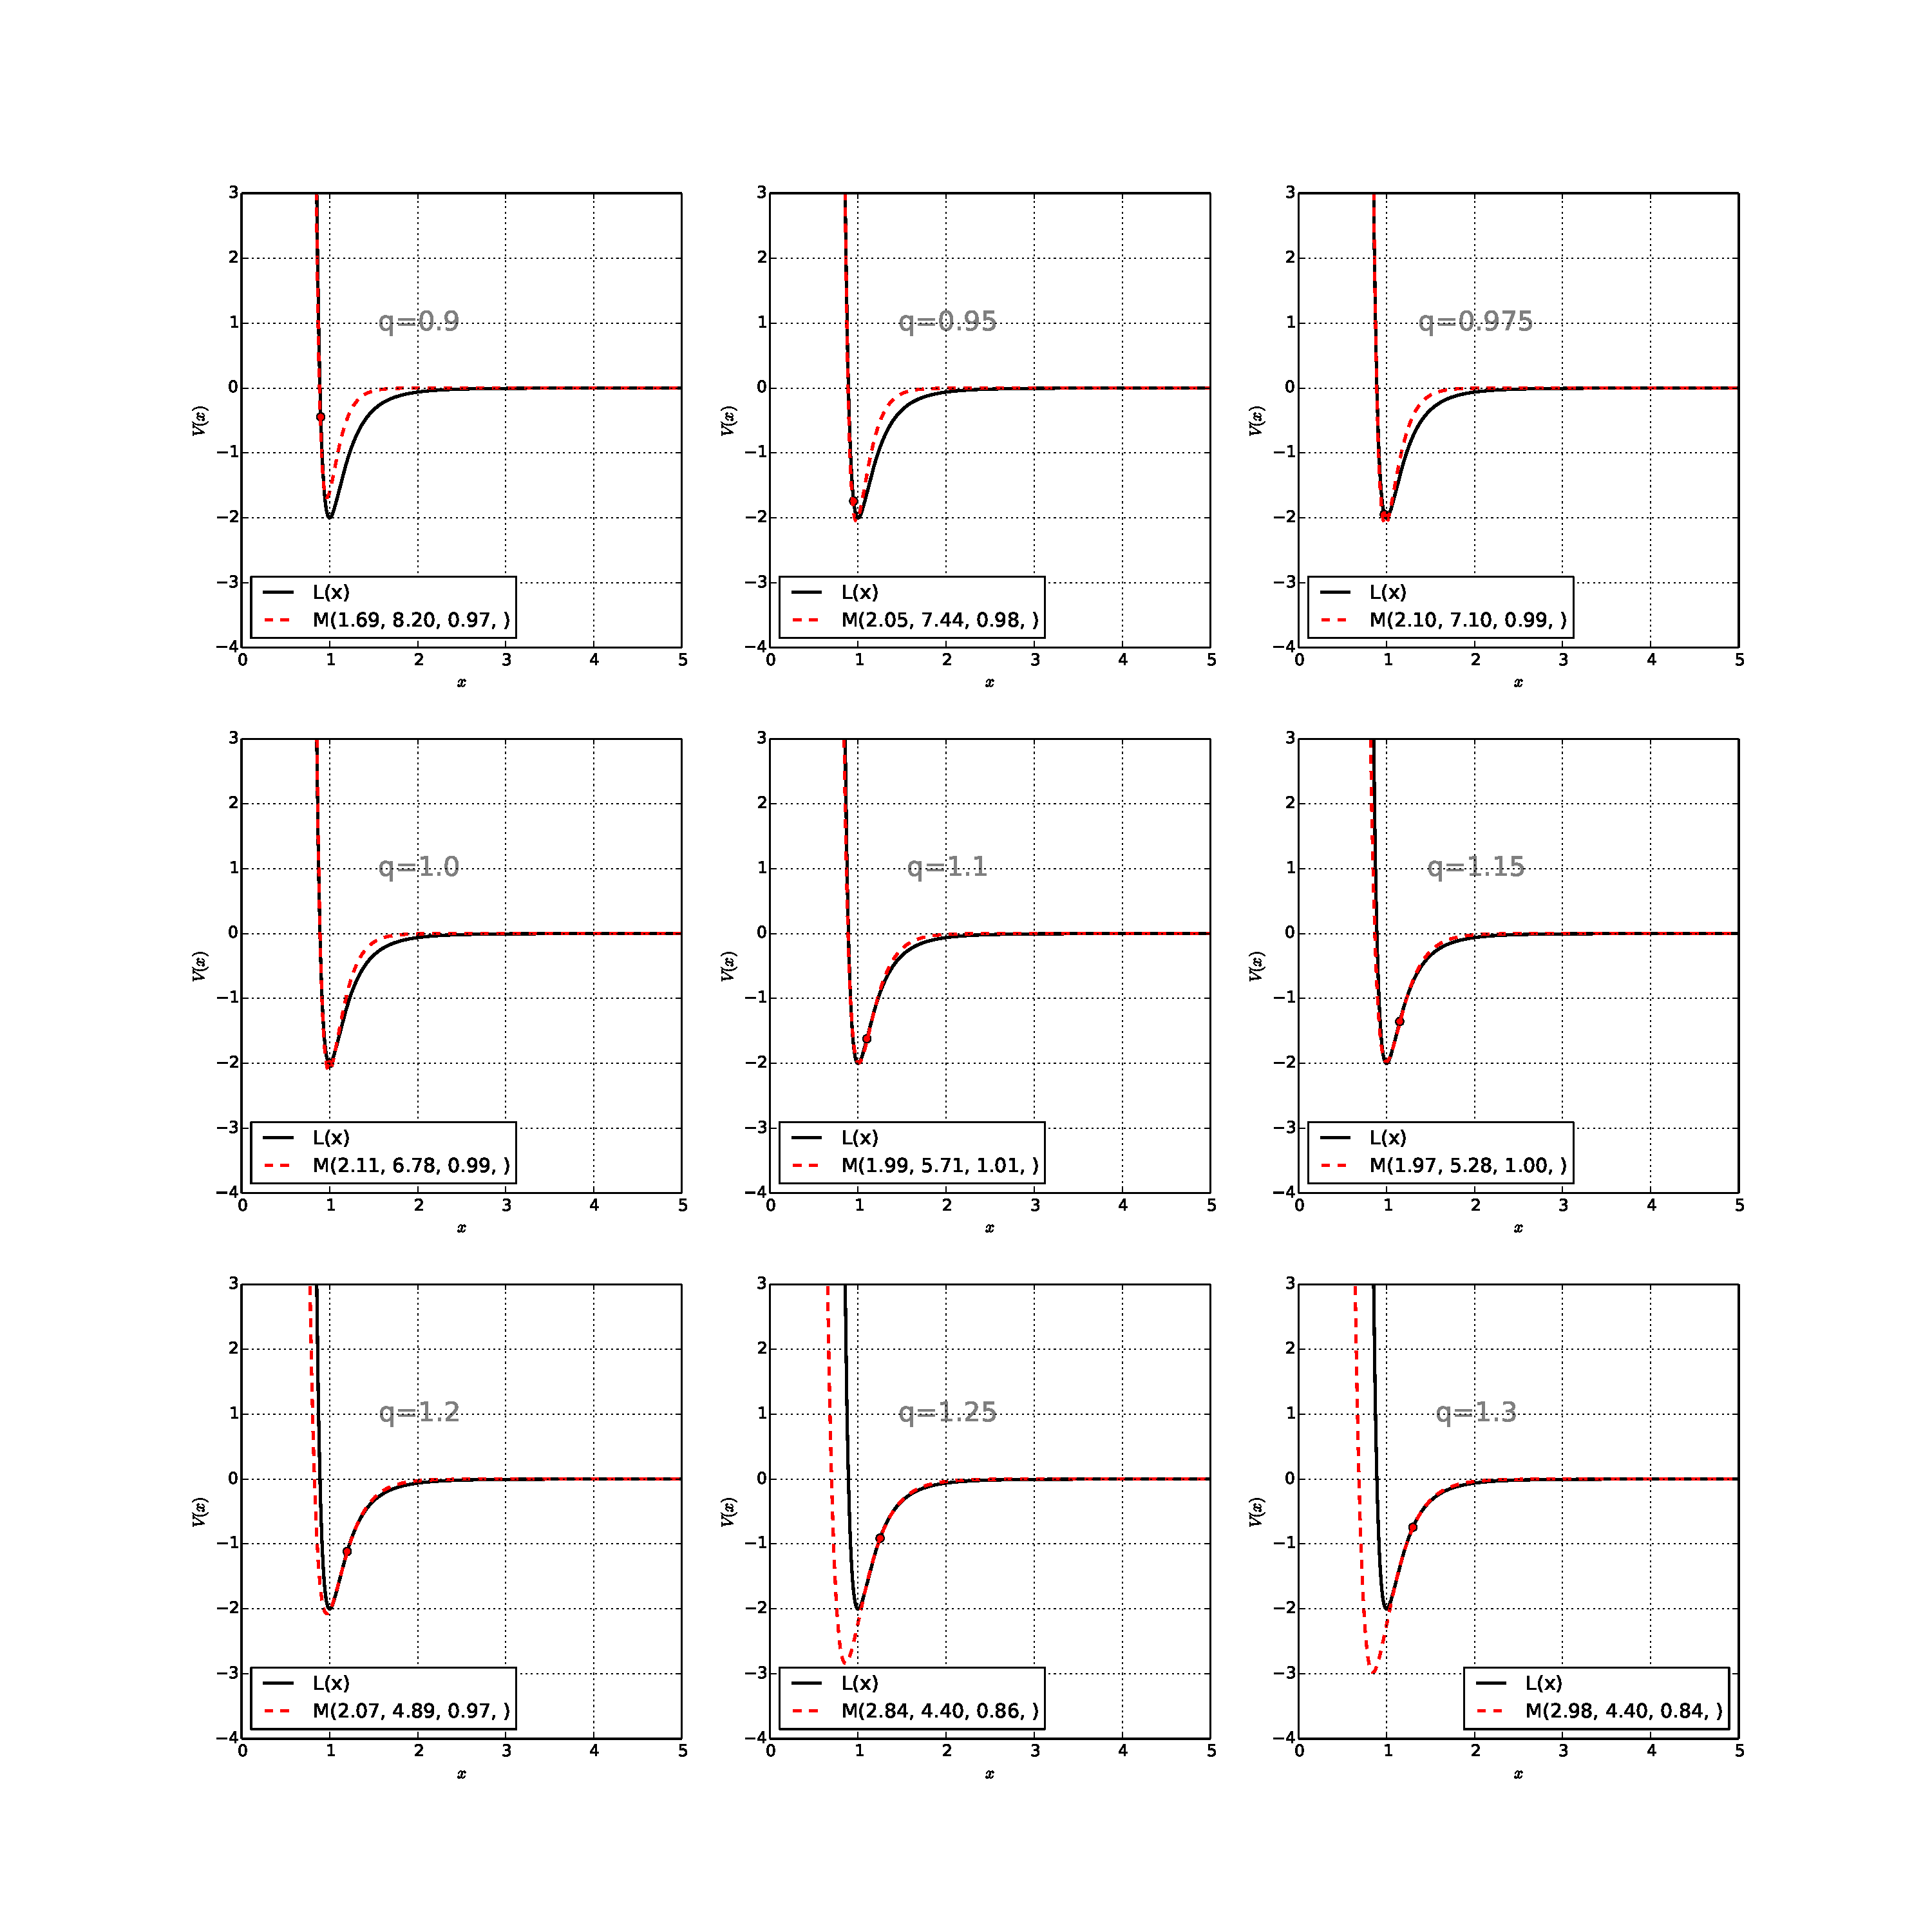
\includegraphics[width=1.0\linewidth]{./figures/MorseFitsLeastsq/fits_leastsq.pdf}
%	\caption[\texttt{leastsq} to the Morse potential]{
%	
%	    \label{fig:MorseFitsLeastsq}
%    }
%
%\end{figure}


\end{chapter}


\clearemptydoublepage

\begin{chapter}{Morse Eigenfunctions}
As a prerequisite for the ladder operators we look at the analytical solution of the Schrödinger equation with the Morse potential
as done in \cite{Landau1981Quantum}. The momentum representation and the moments of the wave function will be shortly calculated.

\section{Analytic Solution} % (fold)
\label{sec:Analytic Solution}
We denote the Morse eigenfunction by $\mu(x)$ and start with the following form of the Schrödinger equation
\begin{equation}
    \mu''(x)+\frac{2}{\varepsilon^4}( E-V_0e^{-2\beta x}+2V_0e^{-\beta x} )\mu(x)=0
\end{equation}

To solve the Schrödinger equation for the Morse potential we first have to transform the  position variable $x$ to get rid of the exponentials:
\begin{equation}
    \label{eq:morse_var_transform}
    z:=\nu e^{-\beta x},\qquad \nu=\sqrt{\frac{8V_0}{\beta^2\varepsilon^4}}
\end{equation}

Furthermore, to simplify notation we introduce an additional constant $s(n,\nu)$, which, using the quantum number $n$, can be written as
\begin{equation}
    \label{eq:const_rel}
    s:=-n+\frac{1}{2}\nu-\frac{1}{2}\; .
\end{equation}

\subsection{Variable Transformation}
Applying the transformation and substituting the new constants yields
\begin{align}
    &\mu''(z)\nu^2\beta^2e^{-2\beta x}+\mu'(z)\nu\beta^2e^{-\beta x}+\frac{2m}{\hbar^2}\left(E-V_0\frac{z^2}{\nu^2}+2V_0\frac{z}{\nu}\right)\mu(z)\\
    &=\mu''(z)z^2+\mu'(z)z+\left[\frac{2m}{\hbar^2\beta^2}E-\underbrace{\frac{2mV_0}{\hbar^2\beta^2}}_{1/4 \nu^2}\frac{z^2}{\nu^2}
	+\underbrace{\frac{4mV_0}{\hbar^2\beta^2}}_{1/2\nu^2}\frac{z}{\nu}\right]\mu(z)\\
    &=\mu''(z)+\frac{\mu'(z)}{z}-\left[\frac{s^2}{z^2}+\frac{1}{4}-\frac{1}{z}\underbrace{\frac{1}{2}\nu}_{n+s+\frac{1}{2}} \right]
    \mu(z)\;,
\end{align}
such that we arrive at the following simplified equation:
\begin{equation}
	\label{eq:morse_transformed_tdse}
	\mu''(z)+\frac{\mu'(z)}{z}+\left( -\frac{1}{4}+\frac{n+s+\frac{1}{2}}{z}-\frac{s^2}{z^2}\right)\mu=0
\end{equation}


\subsection{Asymptotic Solutions}
For solving \eqref{eq:morse_transformed_tdse} we investigate the asymptotics of this equation. For $z\to\infty$ 
\eqref{eq:morse_transformed_tdse} becomes 
\begin{equation}
   \mu_a''(z)=\frac{1}{4}\mu_a(z)
\end{equation}
which is solved by
\begin{equation}
    \mu_a=e^{\pm\frac{1}{2}z}
\end{equation}
and we must chose $\frac{1}{2}$ to obtain a normalizable wave function.\\
Similarly  for $z\to 0$ we have
\begin{equation}
 \mu_a''(z)=\frac{s^2}{z^2}\mu_a(z) 
\end{equation}
solved by
\begin{equation}
    \mu_a(z)=z^{\pm s}
\end{equation}
and we must choose $+s$ to avoid divergence at $z=0$.\\

To account for this asymptotic behavior, we consequently choose the following ansatz:
\begin{equation}
	\label{eq:asymp_ansatz}
	\mu(z)=e^{-\frac{z}{2}}z^{s}w(z)
\end{equation}

After plugging \eqref{eq:asymp_ansatz} into \eqref{eq:morse_transformed_tdse} we obtain the much simpler differential equation
\begin{equation}
	zw''+(2s+1-z)w'+nw=0
\end{equation}
which is solved by the \textit{confluent hypergeometric function} $\mathrm{F}$:
\begin{equation}
    w(z)= {}_{1}F_1(-n;2s+1;z)=L_n^{2s}(z)
\end{equation}
For the special case of $n\in\mathbbm{N}$ this becomes the generalized Laguerre polynomials $\mathrm{L}_{n}^{2s}$
such that we finally arrive at the full solution
\begin{equation}
    \label{eq:morse_function}
  \mu_{n}(z) = N_{n} e^{-\frac{z}{2}} z^{s} \mathrm{L}_{n}^{2s}(z).
\end{equation}
where $s := \frac{\nu - 2n -1}{2}$. The normalization constant $N_n$ will be determined in the next section.\\
Plots of the first few Morse states can be seen in Figures \ref{fig:MorseRe0_2} and \ref{fig:MorseRe0_11}.


\begin{figure}[h!]
	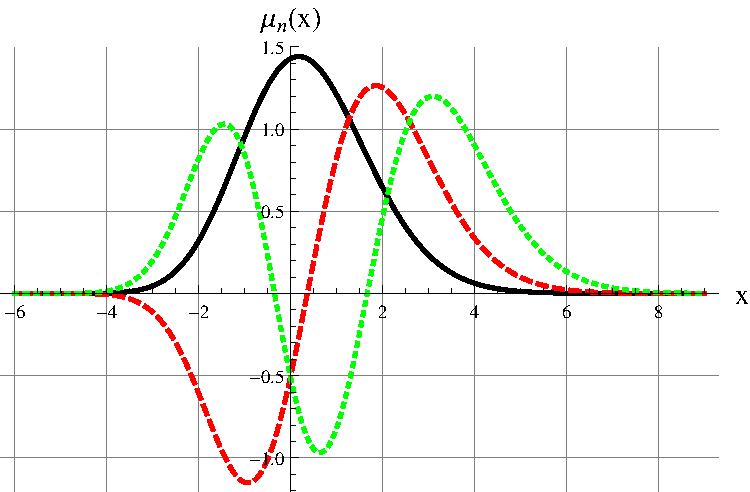
\includegraphics[width=1.0\linewidth]{./figures/MorseWavefunctions/MorseRe0_2.pdf}
       \caption[Morse Wavefunction for $n=0,1,2$]{
	   Plot of the real parts (imaginary part is zero) of the first three Morse eigenstates.
	   (n=0 (solid, black), n=1 (dashed, red), n=2 (dotted, green))\\
	   The parameters $V_0=4.$ and $\beta=0.2$ were chosen.
	\label{fig:MorseRe0_2}
    }

\end{figure}


\begin{figure}[h!]
	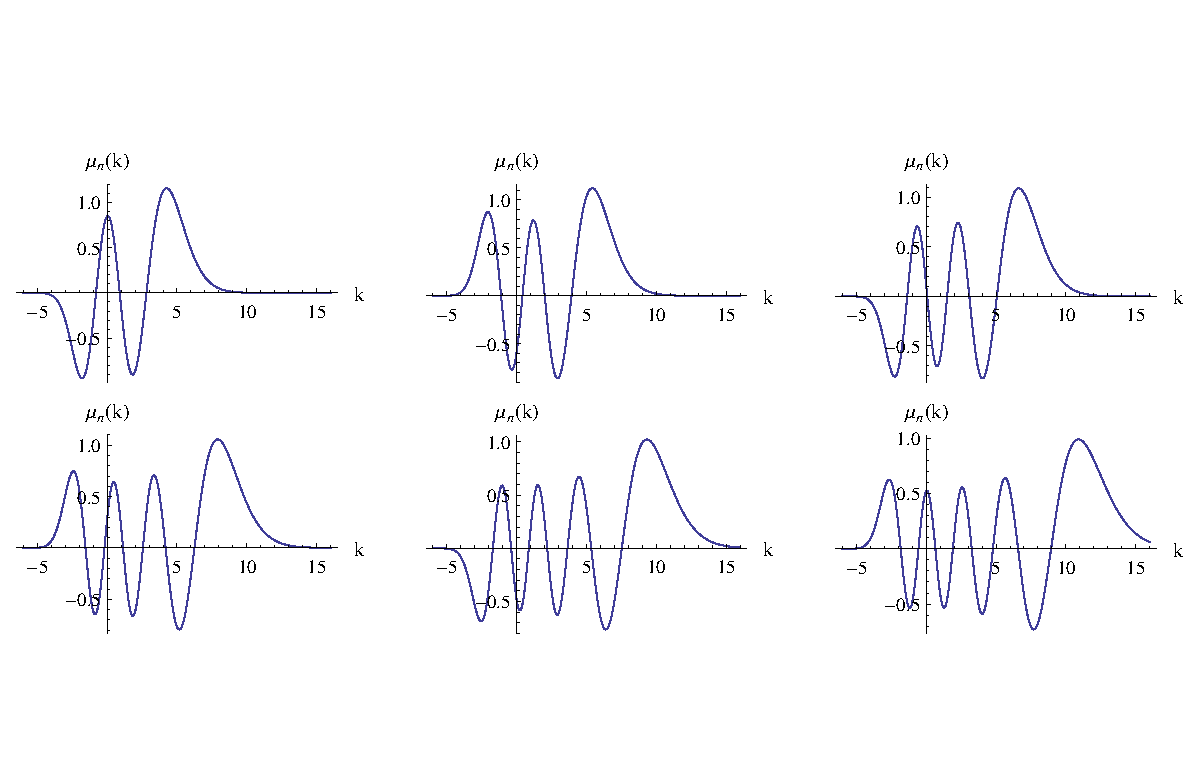
\includegraphics[width=1.0\linewidth]{./figures/MorseWavefunctions/MorseRe0_11.pdf}
       \caption[Morse Wavefunction for $n=3,\ldots,8$]{
	   Higher states of the Morse potential, quantum number $n=3,\ldots,8$ increases from left to right and top to bottom.
	   The parameters $V_0=4.$ and $\beta=0.2$ were chosen.
	\label{fig:MorseRe0_11}
    }

\end{figure}



\subsection{Normalization} % (fold)
\label{sub:Normalization}

In order to calculate the normalization constant $N_n$ we have to compute the following integral
\footnote{Since $\mu_n(z)\in\mathbbm{R}$ we will omit complex conjugation from now on}:
\begin{equation}
  \langle \mu_{m}(x) | \mu_{n}(x) \rangle = \int_{-\infty}^{\infty} \overline{\mu_{m}(x)} \mu_{n}(x) \mathrm{d}x \,.
\end{equation}

Based on the variable transformation \eqref{eq:morse_var_transform} the differential transforms as
\begin{equation}
  \mathrm{d}x = -\frac{1}{\beta z} \mathrm{d}z \,.
\end{equation}
while for the integration boundaries we have
\begin{equation}
  \begin{split}
    z(x) = \infty & \quad x \rightarrow -\infty \\
    z(x) = 0 & \quad x \rightarrow \infty  \,.
  \end{split}
\end{equation}
such that we arrive at the overlap integral
\begin{equation}
  \label{eq:overlap}
  \begin{split}
    \int_{-\infty}^{\infty} \mu_{m}(x) \mu_{n}(x) \mathrm{d}x
    & = - \int_{\infty}^{0} \mu_{m}(z) \mu_{n}(z) \frac{1}{\beta z} \mathrm{d}z \\
    & = \frac{1}{\beta} \int_{0}^{\infty} \mu_{m}(z) \mu_{n}(z) \frac{1}{z} \mathrm{d}z \\
    & =: \frac{1}{\beta} I \,.
  \end{split}
\end{equation}

$I$ can be explicitly written as:
\begin{equation}
  \begin{split}
    I
    & = \int_{0}^{\infty} N_{n} e^{-\frac{z}{2}} z^{s} \mathrm{L}_{n}^{2s}(z) N_{n} e^{-\frac{z}{2}} z^{s} \mathrm{L}_{n}^{2s}(z) \frac{1}{z} \mathrm{d}z \\
    & = N_{n}^{2} \int_{0}^{\infty} e^{-z} z^{2s} \mathrm{L}_{n}^{2s}(z)^{2} \frac{1}{z} \mathrm{d}z \\
    & = N_{n}^{2} \int_{0}^{\infty} e^{-z} z^{\alpha - 1} \mathrm{L}_{n}^{\alpha}(z)^{2} \mathrm{d}z
  \end{split}
\end{equation}
where $\alpha := 2s$. We use the following formula
\footnote{\url{http://functions.wolfram.com/Polynomials/LaguerreL3/21/02/01/0003/}}:
\begin{equation}
  \begin{split}
    I
    & = \int_{0}^{\infty} t^{\alpha - 1} e^{-\lambda t} \mathrm{L}_{m}^{\alpha_{m}}(\lambda t) \mathrm{L}_{n}^{\alpha_{n}}(\lambda t) \mathrm{d}t \\
    & = \frac{\lambda^{-\alpha} \Gamma(\alpha) \Gamma(n-\alpha+\alpha_{n}+1) \Gamma(m+\alpha_{m}+1)}
             {m! n! \Gamma(1-\alpha+\alpha_{n}) \Gamma(\alpha_{m}+1)}
        {}_{3}F_{2}
        \left(
          \begin{matrix}
            - m, \alpha, \alpha - \alpha_{n} \\
            \alpha - \alpha_{n} - n, \alpha_{m} + 1
          \end{matrix}
          \middle| {1} \right) \,.
  \end{split}
\end{equation}

In our case $\lambda = 1$ and for $m = n$ we also have $\alpha_{m} = \alpha_{n}$:
\begin{equation}
  I = \frac{\Gamma(\alpha) \Gamma(n+\alpha_{n}+1) \Gamma(n-\alpha+\alpha_{n}+1)}
           {(n!)^{2} \Gamma(\alpha_{n}+1) \Gamma(\alpha_{n}-\alpha+1)}
      {}_{3}F_{2}
      \left(
        \begin{matrix}
          -n, \alpha, \alpha-\alpha_{n} \\
          -n+\alpha -\alpha_{n}, \alpha_{n}+1
        \end{matrix}
      \middle| {1} \right) \,.
\end{equation}
Defining $\alpha_{n} = \alpha$ yields:
\begin{equation}
  I = \frac{\Gamma(n+\alpha+1)}{\alpha \Gamma(n+1)}
\end{equation}
and using the relation $\alpha := \nu - 2n - 1$:
\begin{equation}
  \label{eq:norm_integral}
  I = \frac{\Gamma(\nu-n)}{(\nu -2n -1) \Gamma(n+1)}
\end{equation}
such that we finally arrive at our normalization constant
\begin{equation}
  N_{n} = \sqrt{\beta \frac{(\nu -2n -1) \Gamma(n+1)}{\Gamma(\nu-n)}} \,.
\end{equation}
% subsection Normalization (end)

\subsection{Orthonormality}

Now starting again from \eqref{eq:overlap} we need to explicitly compute
\begin{equation}
  \begin{split}
    J
    & = \int_{0}^{\infty} N_{m} e^{-\frac{z}{2}} z^{s_{m}} \mathrm{L}_{m}^{2s_{m}}(z)
                          N_{n} e^{-\frac{z}{2}} z^{s_{n}} \mathrm{L}_{n}^{2s_{n}}(z)
                          \frac{1}{z} \mathrm{d}z \\
    & = N_{m} N_{n} \int_{0}^{\infty} e^{-z} z^{s_{m}+s_{n}}
					  \mathrm{L}_{m}^{2s_{m}}(z)
					  \mathrm{L}_{n}^{2s_{n}}(z)
					  \frac{1}{z} \mathrm{d}z \\
	& = N_{m} N_{n} \int_{0}^{\infty} e^{-z} z^{\frac{\alpha_{m}+\alpha_{n}}{2}-1}
					  \mathrm{L}_{m}^{\alpha_{m}}(z)
					  \mathrm{L}_{n}^{\alpha_{n}}(z)
					  \mathrm{d}z
      \end{split}
    \end{equation}
    where $\alpha_{m} := 2s_{m}$ and $\alpha_{n} := 2s_{n}$.
    To solve this integral we use the formula
    \footnote{ \url{http://functions.wolfram.com/Polynomials/LaguerreL3/21/02/01/0002/}}:
    \begin{equation*}
      \begin{split}
	J
	& = \int_{0}^{\infty} t^{\alpha-1} e^{-\lambda t} \mathrm{L}_{m}^{\alpha_{m}}(a_{m} t) \mathrm{L}_{n}^{\alpha_{n}}(a_{n} t) \mathrm{d}t \\
	& = \frac{\lambda^{-\alpha}\Gamma(\alpha) \left(\alpha_{m}+1\right)_{m} \left(\alpha_{n}+1\right)_{n}}{m! n!}
	\sum_{j=0}^{m} \frac{(-m)_{j} (\alpha)_{j}}{\left(\alpha_{m}+1\right)_{j} j!} \left(\frac{a_{m}}{\lambda}\right)^{j}
	\sum_{k=0}^{n} \frac{(-n)_{k} (\alpha+j)_{k}}{\left(\alpha_{n}+1\right)_{k} k!} \left(\frac{a_{n}}{\lambda}\right)^{k} \,.
      \end{split}
    \end{equation*}
    where $a_{m} = 1$, $a_{n} = 1$ and $\lambda = 1$:
    \begin{equation*}
      \begin{split}
	J
	& = \frac{\Gamma(\alpha) \left(\alpha_{m}+1\right)_{m} \left(\alpha_{n}+1\right)_{n}}{m! n!}
	\sum_{j=0}^{m} \frac{(-m)_{j} (\alpha)_{j}}{\left(\alpha_{m}+1\right)_{j} j!}
	\sum_{k=0}^{n} \frac{(-n)_{k} (\alpha+j)_{k}}{\left(\alpha_{n}+1\right)_{k} k!} \\
	& =
	\frac{\alpha_{n}! \Gamma(\alpha) \left(\alpha_{m}+1\right)_{m} \left(\alpha_{n}+1\right)_{n} (\alpha_{n}+\alpha+n)!}
	     {m! n! (\alpha_n-\alpha)! (\alpha_n+n)!}
	{}_{3}F_{2}
	\left(
	  \begin{matrix}
	    -m, \alpha, \alpha-\alpha_{n} \\
	    \alpha_{m}+1, \alpha-\alpha_{n}-n
	  \end{matrix}
	  \middle| {1} \right) \,.
      \end{split}
    \end{equation*}
    Furthermore, inserting $\alpha = \frac{\alpha_{m} + \alpha_{n}}{2}$,
    $\alpha_{m} = \nu - 2m -1$ and $\alpha_{n} = \nu -2n -1$ yields
    \begin{equation}
      J = \frac{\Gamma(\nu-m)}{(\nu-m-n-1) \Gamma(n+1) \Gamma(1+m-n) \Gamma(1-m+n)}
    \end{equation}
    In the case $m = n$ we arrive at \eqref{eq:norm_integral} again.
    Otherwise, using the Euler formula
    \footnote{
      \begin{equation}
	\Gamma(1 + z) \Gamma(1 - z) = \frac{\pi z}{\sin(z \pi)}
      \end{equation}
    }
    the result can be simplified to
    \begin{equation}
      J = \frac{\Gamma(\nu-m)}{(\nu-m-n-1) \Gamma(n+1)}\frac{\sin((m-n)\pi)}{\pi (m-n)}
    \end{equation}
    Now, since  $\sin((m-n)\pi) = 0$ for $m, n \in \mathbb{N}$ it follows, that
    \begin{equation}
      J = 0
    \end{equation}

    % section Analytic Solution (end)

    \section{Momentum Representation} % (fold)
    \label{sec: Momentum Representation}
    Our motivation for calculating the Fourier transformation of the Morse states is the observation in \cite{H_ladder_operators} that in the case of Hagedorn wave packets 
    the variables $(x, q)$ and $(y,p)$, as well as the parameters $Q$ and $P$, up to a sign and a global phase factor simply switch roles in the
    formulas after transformation to momentum space:

\begin{equation}
    \label{eq:HGWavepacketFourier}
    (\mathcal{F}\phi_k(Q, P, \hbar, q, p, x))(y)=(-i)^ke^{-ia\eta/\hbar}\phi_k(Q, P, \hbar, \eta, -q, y)
\end{equation}

Although it might be that this is solely due to the fact that the Gaussians are eigenfunctions of the Fourier transformation it is nevertheless useful to check
if there is any obvious symmetry recognizable in the Morse case after transformation.\\
Apart from that the results might also be useful to compute certain matrix elements in future applications.\\

We recall that the  Morse wave packet $\mu_{n}$ is given by:

\begin{equation}
  \mu_{n}(z) = N_{n} e^{-\frac{z}{2}} z^{s} L_{n}^{2s}(z)
\end{equation}

and with $z = \nu \exp(-\beta x)$ we have:

\begin{equation}
  \mu_{n}(x) = N_{n} e^{-\frac{\nu}{2} \exp(-\beta x)} \nu^{s} \exp(-\beta x)^{s} L_{n}^{2s}\left(\nu \exp(-\beta x)\right)
\end{equation}

\subsection{Ground State}
Since for $n=0$ the Laguerre polynomials equal unity, we first try to compute the Fourier transformation of the ground state $\mu_{0}$:

\begin{equation}
  \mu_{0}(x) = N_{0} e^{-\frac{\nu}{2} \exp(-\beta x)} \nu^{s} \exp(-\beta x)^{s} \underbrace{L_{n}^{2s}\left(\nu \exp(-\beta x)\right)}_{\equiv 1}
\end{equation}

which is proportional to the following kernel:

\begin{equation}
  \mu_{0}(x) \sim e^{-\alpha e^{-\beta x}} \left(e^{-\beta x}\right)^{\gamma}
\end{equation}

where $\alpha = \frac{\nu}{2}$ and $\gamma = s$. Next we try to compute its
Fourier transformation:

\begin{align}
  \ft{e^{-\alpha e^{-\beta x}} \left(e^{-\beta x}\right)^{\gamma}}(k)
  & = \frac{1}{\sqrt{2\pi}} \int_{-\infty}^{\infty} e^{-\alpha e^{-\beta x}} \left(e^{-\beta x}\right)^{\gamma} e^{- i k x} \di{x} \\
  & = \frac{1}{\sqrt{2\pi}}
  \frac{1}{\beta}
  \alpha^{-\gamma -\frac{i k}{\beta}}
  \Gamma \left(\gamma+\frac{i k}{\beta}\right) \,.
\end{align}

Finally we get the transformation of the wave packet $\mu_{0}$:

\begin{equation*}
  \hat{\mu_{0}}(k) = \ft{\mu_{0}(x)} =
  \frac{N_{0}}{\sqrt{2\pi}}
  \frac{\nu^{s}}{\beta}
  \left(\frac{\nu}{2}\right)^{-s -\frac{i k}{\beta}}
  \Gamma \left(s+\frac{i k}{\beta}\right)
\end{equation*}

\subsection{Higher States}

Next we look at the higher order states $n>0$. This time we need to include
the Laguerre polynomial $L_{n}^{a}(x)$. In order to so we choose the following representation of the Laguerre polynomials:

\begin{equation}
  L_{n}^{a}(z) := \sum_{i=0}^{n} \frac{(-1)^{i}}{i!}
                                \frac{\Gamma(n+a+1)}{\Gamma(a+1+i) \Gamma(n+1-i)}
                                z^{i}
                = \sum_{i=0}^{n} C_{n,a,i} \, z^{i} \,.
\end{equation}

Applying again the coordinate transformation we find that:

\begin{equation}
  L_{n}^{2s}(z)
  = L_{n}^{2s}\left(\nu \exp(-\beta x)\right)
  = \sum_{i=0}^{n} C_{n,2s,i} \, \left(\nu \exp(-\beta x)\right)^{i}
\end{equation}

and since $i$ is a nonnegative integer we have:

\begin{equation}
  L_{n}^{2s}(x) = \sum_{i=0}^{n} C_{n,2s,i} \, \nu^{i} \exp(- i \beta x) \,.
\end{equation}

The higher order states $\mu_{n}(x)$ can therefore be written like:

\begin{align}
  \mu_{n}(x)
  & = N_{n} e^{-\frac{\nu}{2} \exp(-\beta x)} \nu^{s} \exp(-\beta x)^{s} \sum_{i=0}^{n} C_{n,2s,i} \, \nu^{i} \exp(- i \beta x) \\
  & = \sum_{i=0}^{n} N_{n} C_{n,2s,i} \, \nu^{s+i} e^{-\frac{\nu}{2} \exp(-\beta x)} \exp(-\beta x)^{s} \exp(- i \beta x) \,.
\end{align}

We can compute the Fourier transformation of a slightly extended kernel:

\begin{align}
  \ft{e^{-\alpha e^{-\beta x}} \left(e^{-\beta x}\right)^{\gamma} e^{- i \beta x}}(k)
  & = \frac{1}{\sqrt{2\pi}}
  \frac{1}{\beta}
  \alpha^{-\gamma -i -\frac{i k}{\beta}}
  \Gamma \left(\gamma+i+\frac{i k}{\beta}\right) \,.
\end{align}

For the wave packet we in turn find:

\begin{equation}
  \hat{\mu_{n}}(k) = \ft{\mu_{n}(x)} =
  \sum_{i=0}^{n}
  N_{n} C_{n,2s,i} \, \nu^{s+i}
  \frac{1}{\sqrt{2\pi}}
  \frac{1}{\beta}
  \left(\frac{\nu}{2}\right)^{-s -i -\frac{i k}{\beta}}
  \Gamma \left(s+i+\frac{i k}{\beta}\right)
\end{equation}

where the constant is $C_{n,2s,i} = \frac{(-1)^{i}}{i!} \frac{\Gamma(n+2s+1)}{\Gamma(2s+1+i) \Gamma(n+1-i)}$. It is indeed possible to resolve this sum and obtain a relatively simple formula:

\begin{equation*}
  \hat{\mu}_{n}(k) =
  \frac{N_{n}}{\sqrt{2\pi}}
  \frac{2^{s+\frac{i k}{\beta}} \nu^{-\frac{i k}{\beta}}}{\beta}
  \frac{\Gamma(1+n+2s)}{\Gamma(1+n)\Gamma(1+2s)}
  \Gamma\left(s+\frac{i k}{\beta}\right)
  {}_{2}F_{1}
  \left(
    \begin{matrix}
      - n, s + \frac{i k}{\beta} \\
      2s + 1
    \end{matrix}
    \middle| {2} \right)
\end{equation*}

Again we provide some plots of the Morse states in the Figures

\begin{figure}[h!]
	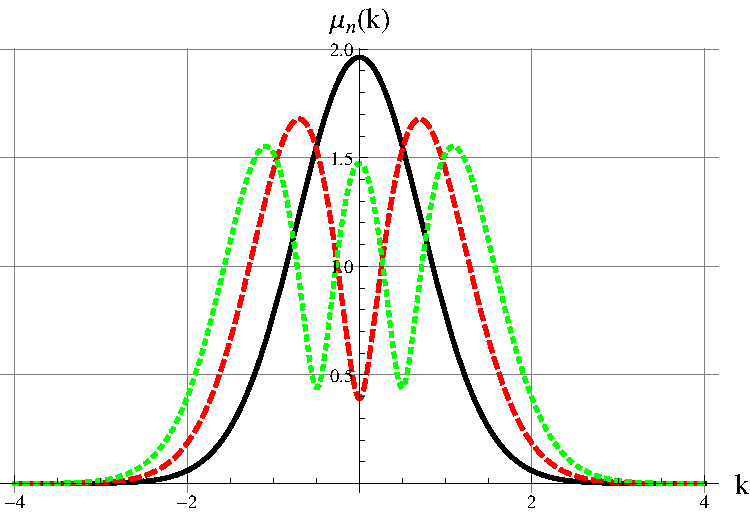
\includegraphics[width=1.0\linewidth]{./figures/MorseFourier/FourierAbsn0_2.pdf}
       \caption[Morse momentum wavefunction for $n=0,1,2$]{
	   Plot of the absolute modulus of the first three Morse eigenstates in momemtum space
	   (n=0 (solid, black), n=1 (dashed, red), n=2 (dotted, green))\\
	   The parameters $V_0=4.$ and $\beta=0.2$ were chosen.
	\label{fig:FourierAbsn0_2}
    }

\end{figure}


\begin{figure}[h!]
	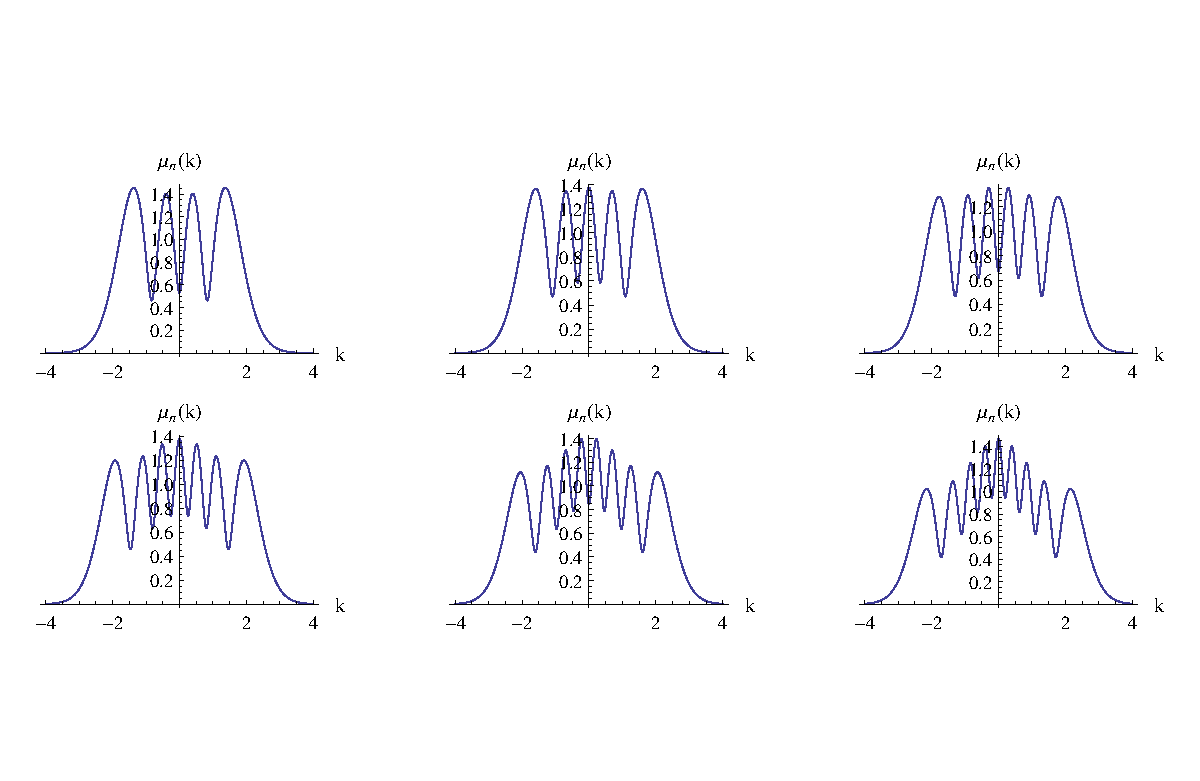
\includegraphics[width=1.0\linewidth]{./figures/MorseFourier/FourierAbsn0_11.pdf}
       \caption[Morse momentum wavefunction for $n=3,\ldots,8$]{
	   Higher states of the Morse potential in momentum space, quantum number $n=3,\ldots,8$ increases from left to right and top to bottom.
	   The parameters $V_0=4.$ and $\beta=0.2$ were chosen.
	\label{fig:FourierAbsn0_11}
    }

\end{figure}


% section Momentum Representation (end)

\section{Moments} % (fold)
\label{sec:Moments}
As explained in the introduction, the parameters $Q$ and $P$ can be interpreted as the width in position and momentum space, respectively.
Since the probability distribution $|\mu_n|^2$ describes the localization of the particle, calculating its first two central moments 
provides us with analytical expressions for the mean position and standard deviation. This might again give hints about the parameters.
In addition to that we also calculate some important diagonal matrix elements for the Morse function which we will then, using the ladder operator
formalism introduced in the next section, generalize to other operators.\\

We start again with the following expression
\begin{equation}
  \mu_{n}(x) = N_{n} e^{-\frac{\nu}{2} \exp(-\beta x)} \nu^{s} \exp(-\beta x)^{s} L_{n}^{2s}\left(\nu \exp(-\beta x)\right)\;.
\end{equation}


The following properties about the various parameters hold:
\begin{align}
  & n \in \mathbb{N} \\
  & \beta \in \mathbb{R}, \beta > 0 \\
  & V_{0} \in \mathbb{R}, V_{0} > 0 \\
  & N_{n} \in \mathbb{R} \,,
\end{align}

from the condition $\nu - 2n - 1 =: w > 0$ and $s := \frac{w}{2}$ we find that:

\begin{align}
  & \nu \in \mathbb{R}, \nu > 0 \\
  & s \in \mathbb{R}, s > 0 \,.
\end{align}

\subsection{First moment of the ground state}

The task is to compute the first moment:

\begin{equation}
  \braket{\mu_{0} | x | \mu_{0}} = \int_{-\infty}^{\infty} \mu_{0}(x) x \mu_{0}(x) \di{x} \,.
\end{equation}

With:

\begin{equation}
  \mu_{0}(x) = N_{0} \underbrace{e^{-\frac{\nu}{2} e^{-\beta x}}}_{A(x)} \nu^{s} \underbrace{\left(e^{-\beta x}\right)^{s}}_{B(x)}
\end{equation}

we find:

\begin{align}
    \int_{-\infty}^{\infty} \mu_{0(x)} x \mu_{0}(x) \di{x}
  & =   \int_{-\infty}^{\infty} N_{0} \nu^{s} A(x) B(x) x N_{0} \nu^{s} A(x) B(x) \di{x} \\
  & =   N_{0}^{2} \nu^{2s} \int_{-\infty}^{\infty} A(x) B(x) x A(x) B(x) \di{x} \\
  & =   N_{0}^{2} \nu^{2s} \int_{-\infty}^{\infty} A(x)^{2} B(x)^{2} x \di{x} \,.
\end{align}

The last equality holds since $A(x)$ and $B(x)$ are real valued.
This integral can be written in general form like shown in \eqref{int:def_1}
and substitution of $\alpha=\nu$ and $\gamma=2s$ gives for the first moment:

\begin{equation}
    \braket{\mu_{0} | x | \mu_{0}}
    = \frac{N_{0}^{2}}{\beta^{2}} \Gamma(\nu-1) \left(\log(\nu) - \psi^{(0)}(\nu-1)\right)
\end{equation}
where for $n=0$ we have by definition $2s = \nu - 1$ and $\psi^{(i)}$ denotes the polygamma function of
order $i$ defined as the $i+1$-th derivative of the logarithm of the gamma function:
\begin{align}
\psi^{(i)}(z)=\pdiff{^{m+1}}{z^{m+1}}\log \Gamma(z)
\end{align}



\subsection{Second moment of the ground state}


For the second central moment we have:

\begin{equation}
  \braket{\mu_{0} | (x-q)^{2} | \mu_{0}}
  = \braket{\mu_{0} | x^{2} | \mu_{0}}
  - 2 q \braket{\mu_{0} | x | \mu_{0}}
  + q^{2} \braket{\mu_{0} | \mu_{0}}
\end{equation}

hence we first compute:

\begin{align}
  \braket{\mu_{0} | x^{2} | \mu_{0}}
  & = \int_{-\infty}^{\infty} \conj{\mu_{0(x)}} x^{2} \mu_{0}(x) \di{x} \\
  & =   N_{0}^{2} \nu^{2s} \int_{-\infty}^{\infty} A(x)^{2} B(x)^{2} x^{2} \di{x} \,.
\end{align}

The basic integral we need here is given in \eqref{int:def_2} and
applying the same substitution of $\alpha=\nu$ and $\gamma=2s$ again
 gives the second moment:

\begin{align}
    \braket{\mu_{0} | x^{2} | \mu_{0}}
    = \frac{N_{0}^{2}}{\beta^{3}} \Gamma(\nu-1) \left(\left(\log(\nu) - \psi^{(0)}(\nu-1) \right)^{2} + \psi^{(1)}(\nu-1) \right)
\end{align}


\subsection{Moments of higher states}


The aim of this section is the computation of $k$-th moments for higher states $\mu_{n}$.
This is not straight-forward but can be done step by step. We start with:

\begin{align}
  \label{eq:def_kth_mom}
  \braket{\mu_{n} | x^{k} | \mu_{n}}
  & = \int_{-\infty}^{\infty} \conj{\mu_{n}(x)} x^{k} \mu_{n}(x) \di{x} \\
  & = \int_{-\infty}^{\infty} \conj{N_{n} \nu^{s} A(x) B(x) L_{n}^{2s}(\delta)}
                                \, x^{k} \,
                                N_{n} \nu^{s} A(x) B(x) L_{n}^{2s}(\delta) \,\di{x} \\
  & =   N_{n}^{2} \nu^{2s} \int_{-\infty}^{\infty} A(x)^{2} B(x)^{2} \left( L_{n}^{2s}(\delta) \right)^{2} x^{k} \,\di{x}
\end{align}

where $\delta := \nu \exp(-\beta x)$. Before we can continue we need an explicit expansion
for the square of Laguerre polynomials. This is a classical result by W. N. Bailey
and W. T. Howell\footnote{
We use the following definition of Laguerre polynomials:
\begin{equation*}
  L_{n}^{a}(z)
  :=
  \frac{\Gamma(n+a+1)}{\Gamma(n+1) \Gamma(a+1)}
  \,
  {}_{1}F_{1}
  \left(
    \begin{matrix}
      - n \\
      a+1
    \end{matrix}
    \middle| {x} \right)
\end{equation*}
and have to divide by an additional factor $\Gamma(a+1)$ compared to the original paper.}:

\begin{align}
  \left( L_{n}^{a}(z) \right)^{2}
  & =
  \underbrace{\frac{\Gamma(1+n+a)}{\Gamma(1+a) 2^{2n}n!}}_{=: G_{n,a}}
  \sum_{r=0}^{n}
  \underbrace{\frac{(2r)! (2n-2r)!}{\Gamma(1+r) \Gamma(1+n-r)^{2} \Gamma(1+r+a)}}_{=: F_{n,a,r}}
  L_{2r}^{2a}(2z) \\
  & =
  G_{n,a} \sum_{r=0}^{n} F_{n,a,r} L_{2r}^{2a}(2z) \,.
\end{align}

Combining this with the explicit expression for the Laguerre polynomials:

\begin{equation}
  L_{n}^{a}(z)
  :=
  \sum_{i=0}^{n}
  \underbrace{
    \frac{(-1)^{i}}{i!}
    \frac{\Gamma(n+a+1)}{\Gamma(a+1+i) \Gamma(n+1-i)}
  }_{=: C_{n,a,i}}
  z^{i}
  = \sum_{i=0}^{n} C_{n,a,i} \, z^{i} \,.
\end{equation}

we find:

\begin{equation}
  \left( L_{n}^{a}(z) \right)^{2} =
  G_{n,a}
  \sum_{r=0}^{n}
  F_{n,a,r} \,
  \sum_{i=0}^{2 r}
  C_{2r,2a,i} \, (2 z)^{i} \,.
\end{equation}

Plugging this into the integral \eqref{eq:def_kth_mom} from above yields:

\begin{align*}
  \braket{\mu_{n} | x^{k} | \mu_{n}}
  & =
  N_{n}^{2} \nu^{2s} \int_{-\infty}^{\infty} A(x)^{2} B(x)^{2}
  G_{n,2s} \sum_{r=0}^{n} F_{n,2s,r} \sum_{i=0}^{2 r} C_{2r,4s,i} \, (2 \delta)^{i} x^{k} \di{x} \\
  & =
  N_{n}^{2} \nu^{2s} G_{n,2s} \sum_{r=0}^{n} \sum_{i=0}^{2 r} F_{n,2s,r} \, C_{2r,4s,i} \, 2^{i}
  \int_{-\infty}^{\infty} A(x)^{2} B(x)^{2} \delta^{i} x^{k} \di{x} \\
  & =
  N_{n}^{2} \nu^{2s} G_{n,2s} \sum_{r=0}^{n} \sum_{i=0}^{2 r} F_{n,2s,r} \, C_{2r,4s,i} \,
  2^{i} \nu^{i}
  \int_{-\infty}^{\infty} A(x)^{2} B(x)^{2} \left(e^{-\beta x}\right)^{i} x^{k} \di{x}
\end{align*}

For the remaining integrals we use the general formula given in
\eqref{int:def_n} with the values $\alpha = \nu$ and $\gamma = 2s + i$.

\begin{align}
    \braket{\mu_{n} | x^{k} | \mu_{n}}
    =
    N_{n}^{2} \nu^{2s} G_{n,2s}
    \sum_{r=0}^{n}
    \sum_{i=0}^{2 r}
    F_{n,2s,r} \, C_{2r,4s,i} 2^{i} \nu^{i} I_{\nu,\beta,2s+i}^{(k)} \,.
\end{align}

Next we try to combine the individual parameter terms and resolve the sums.
However, it seems that this is not possible and there exists no closed form
for this nested sum.

% section Moments (end)

\end{chapter}


\clearemptydoublepage

\begin{chapter}{Ladder operators for the Morse Potential}
In this chapter we derive the explicit form of the ladder operators for the Morse eigenfunctions,
following \cite{Dong_ladder_operators}.\\
As already mentioned in \ref{sec:morse_potential}, the Morse potential allows for a continuum of free states as well as a finite number of discrete bound states. In our case, only the bound 
solutions are of interest.


\section{Construction} % (fold)
\label{sec:Construction}
Dong starts by looking for differential operators of the form
\begin{equation}
    \label{eq:dong_operator_form}
    \hat{\mathcal{K}}_{\pm}=A_{\pm}(z)\diff{}{z}+B_{\pm}(z)
\end{equation}
with the property that
\begin{align}
    \hat{\mathcal{K}}_{\pm}\mu_n(z)&=k_{\pm}\mu_{n\pm 1}(z)\\
	\hat{\mathcal{K}}_{-}\mu_0&\equiv 0\\    
    \hat{\mathcal{K}}_{+}\mu_{\text{max}}&\equiv 0\;,
\end{align}
where $\mu_0$ and $\mu_{\text{max}}$ are referring to the lowest and highest Morse eigenfunction,
respectively.\\

Application of the differential operator $\mathrm{d}/\mathrm{d}z$ to the $n$-th Morse eigenfunction \eqref{eq:morse_function} leads to
\begin{equation}
    \label{eq:dong_apply_ddy}
    \diff{}{z}\mu_n(z)=-\frac{1}{2}\mu_n(z)+\frac{1}{z}s\mu_n(z)+N_n e^{-z/2}z^s\diff{}{z}\mathrm{L}_n^{2s}(z).
\end{equation}
where $\mathrm{L}_n^{2s}(z)$ denotes the n-th generalized Laguerre polynomial.\\

Using the recursion relation
\begin{equation}
	\label{eq:dong_ddy_rek}
	\diff{}{z}\mathrm{L}_{n}^\alpha(z)=-\frac{1}{\alpha+1}\left(z\mathrm{L}_{n-1}^{\alpha+2}(z)+n\mathrm{L}_{n}^\alpha(z)\right)
\end{equation}
taken from \cite{DongFactMethods} and substituting it into \eqref{eq:dong_apply_ddy} yields
\begin{equation}
    \left(\diff{}{z}(2s+1)-\left(\frac{1}{z}s-\frac{1}{2}\right)(2s+1)+n\right)\mu_n(z)=-\frac{N_n}{N_{n-1}}\mu_{n-1}(z) \;,
\end{equation}
such that the lowering operator\footnote{
    In \cite{Dong_ladder_operators} these operators are denoted as $\hat{K}_{\pm}$, while we choose to follow the notation in \cite{FGL_semiclassical_dynamics} 
    and use $\mathcal{L}$ for the lowering and $\mathcal{R}$ for the raising operator, respectively.}
can be defined as
\begin{equation}
    \label{eq:dong_lop}
    \mathcal{L}:=-\left(\diff{}{z}(2s+1)-\frac{1}{z}s(2s+1)+\frac{\nu}{2} \right)\sqrt{\frac{s+1}{s}}
\end{equation}
whose action on a Morse eigenfunction $\mu_n$ is given by
\begin{equation}
    \label{eq:dong_lop_action}
    \mathcal{L}\mu_n(z)=l\mu_{n-1}(z),\quad l=\sqrt{n(\nu-n)}\; .
\end{equation}

For the raising operator using \eqref{eq:dong_apply_ddy} again as well as the relations
\begin{align}
    &    z\diff{}{z}\mathrm{L}_n^\alpha(z)=n\mathrm{L}_n^{\alpha}(z)-(n+\alpha)\mathrm{L}_{n-1}^{\alpha}(z)\\
    &	(n+1)\mathrm{L}_{n+1}^{\alpha}(z)-(2n+\alpha+1-z)\mathrm{L}_n^{\alpha}(z)+(n+\alpha)\mathrm{L}_{n-1}^{\alpha}(z)=0\\
    &	\mathrm{L}_n^{\alpha-1}(z)=\mathrm{L}_n^{\alpha}(z)-\mathrm{L}_{n-1}^{\alpha}(z)
\end{align}
the following expression is found
\begin{equation}
    \label{eq:dong_rop}
    \mathcal{R}:=\left(\diff{}{z}(2s-1)+\frac{1}{z}s(2s-1)-\frac{\nu}{2} \right)\sqrt{\frac{s-1}{s}}
\end{equation}
with the corresponding action
\begin{equation}
    \label{eq:dong_rop_action}
    \mathcal{R}\mu_n(z)=r\mu_{n+1}(z),\quad r=\sqrt{(n+1)(\nu-n-1)}\; .
\end{equation}
% section Construction (end)

\section{Lie Algebra} % (fold)
\label{sec:LieAlgebra}
Next, calculating the commutator of the two ladder operators yields
\begin{equation}
    \label{eq:dong_commutator}
    [\mathcal{R},\mathcal{L}]\mu_n(z)=2k_0\mu_n(z)
\end{equation}
with eigenvalue
\begin{equation}
    \label{eq:dong_k0_ev}
    k_0=n-\frac{\nu-1}{2}\;,
\end{equation}
which can be rearranged to yield
\begin{equation}
\label{eq:dong_k0_ev2}
\frac{\nu}{2}=n-k_0-\frac{1}{2}\;.
\end{equation}

This can be plugged into the differential equation for the Morse potential \eqref{eq:morse_transformed_tdse} such that we obtain
\begin{equation}
\left( z\frac{\mathrm{d}^{2}}{\mathrm{d}z^{2}}+\diff{}{z}-\frac{s^2}{z}-\frac{z}{4}+n+\frac{1}{2} 
-k_0 \right)\mu_n=0\; .
\end{equation}

If we define the operator $\mathcal{K}_0$ as
\begin{equation}
    \mathcal{K}_0:=\left( z\frac{\mathrm{d}^{2}}{\mathrm{d}z^{2}}+\diff{}{z}-\frac{s^2}{z}-\frac{z}{4}+n+\frac{1}{2}  \right)\;
\end{equation}
we get the following eigenvalue equation
\begin{equation}
\label{eq:dong_k0eveq}
\mathcal{K}_0\mu_n=k_0\mu_n\; .
\end{equation}

Finally, comparing \eqref{eq:dong_k0eveq} and \eqref{eq:dong_commutator}, we can identify
$\mathcal{K}_0$ with the commutator $[\mathcal{R},\mathcal{L}]$ of $\mathcal{R}$ and $\mathcal{L}$. These three operators form a closed Lie algebra, which by their commutation relations
\begin{align}
    \begin{split}
	[\mathcal{R},\mathcal{L}]=2\mathcal{K}_0,\quad  [\mathcal{K}_0,\mathcal{L}]=-\mathcal{L},\quad
	[\mathcal{K}_0,\mathcal{R}]=\mathcal{R}      
    \end{split}
\end{align}
can also be identified as being isomorphic to the angular momentum algebra $\mathfrak{su}(2)$.\\

Finally, as we have seen in section \ref{sub:DiagonalizationHGHam}, an essential step towards the implementation of a time stepping algorithm is the 
factorization of the Hamiltonian using ladder operators because this will give us the connection to the wave packet parameter evolution.\\

In terms of this algebra of $SU(2)$ the Hamiltonian can be written as:
\begin{equation}
    \label{eq:DongHamiltonian}
    \mathcal{H}=-\frac{\hbar \omega}{\nu}\mathcal{K}_0^2\;,\qquad \omega=\frac{\hbar\beta^2\nu}{2\mu}
\end{equation}

This looks quite compact, but expanding the square and the commutator in terms of the ladder operators $\mathcal{R}$ and $\mathcal{L}$ 
we unfortunately get something more complicated than the simple anti-commutator expression \eqref{eq:HG_OpHamiltonian} in the Hagedorn case.


\section{Three-Term Recursion} % (fold)
\label{sec:ThreeTermRecursion}
Following the procedure in \cite{FGL_semiclassical_dynamics}, we will use \eqref{eq:dong_lop} and \eqref{eq:dong_rop} to obtain a three-term recursion
relation for the Morse eigenfunctions $\mu_n$. This relation is used for the fast and stable numerical evaluation of the Morse functions.\\

As a first step we can express the differential operator $\mathrm{d}/\mathrm{d}z$ in terms of our ladder operators $\mathcal{L}$ and $\mathcal{R}$:
\begin{equation}
    \label{eq:dong_ddyinLR}
    \diff{}{z}=\mathcal{R}\left(\frac{1}{2(2s-1)}\sqrt{\frac{s}{s-1}}\right)-\mathcal{L}\left(\frac{1}{2(2s+1)}\sqrt{\frac{s}{s+1}}\right)
    +\frac{\nu}{2(2s+1)(2s-1)}
\end{equation}
We then can eliminate this operator from \eqref{eq:dong_lop} and \eqref{eq:dong_rop} such that we get
\begin{align}
    \mathcal{L}=-\sqrt{\frac{s+1}{s-1}}\frac{2s+1}{2s-1}\mathcal{R}
    +\sqrt{\frac{s+1}{s}}\frac{2s}{2s-1}\left(\frac{4s^2-1}{z}-\nu\right)\label{eq:dong_lop2}\\
    \mathcal{R}=-\sqrt{\frac{s-1}{s+1}}\frac{2s-1}{2s+1}\mathcal{L}
    +\sqrt{\frac{s-1}{s}}\frac{2s}{2s+1}\left(\frac{4s^2-1}{z}-\nu\right)\label{eq:dong_rop2}
\end{align}

Next, reordering \eqref{eq:dong_rop_action} and substituting \eqref{eq:dong_rop2} yields
\begin{align}
    \mu_{n+1} &= \frac{1}{r}\mathcal{R}\mu_n\\
    &=\frac{1}{r}\left(-\sqrt{\frac{s-1}{s+1}}\frac{2s-1}{2s+1}\mathcal{L}
	+\sqrt{\frac{s-1}{s}}\frac{2s}{2s+1}\left(\frac{4s^2-1}{z}-\nu\right)\right)\mu_n
\end{align}
and finally, after substituting \eqref{eq:dong_lop_action} we obtain the desired three-term relation
\begin{equation}
    \mu_{n+1}=\frac{1}{r}\sqrt{\frac{s-1}{s}}\frac{2s}{2s+1}\left(\frac{4s^2-1}{z}-\nu\right)\mu_n
    -\frac{l}{r}\sqrt{\frac{s-1}{s+1}}\frac{2s-1}{2s+1}\mu_{n-1}
\end{equation}

The n-th state can then be explicitly written as
\begin{equation}
\mu_n(z)=\mathcal{N}_n\mathcal{R}^n\mu_0(z),\quad \mathcal{N}_n:=\sqrt{\frac{(\nu-n-1)!}{n!(\nu-1)!}}
\end{equation}

% section Three-Term Recursion (end)

\section{Back Transformation to original position space} % (fold)
\label{sec:Back_transf}
Our original physical position variable was exponentially rescaled in order to solve the differential equation and construct the ladder operators.
However, for the numerical treatment, especially the time stepping, this might cause problems.
Hence, we also provide a representation of the operators in the original $x$ domain.\\

Using the transformation $z=\nu\exp{(-\beta x)}$ we obtain the following transformed expression for the differential operator
\begin{equation}
    \label{eq:ddy}
    \diff{}{x}=-\beta z\diff{}{z}\;,
\end{equation}
such that the back transformation of the $\mathcal{L}$ and $\mathcal{R}$ operators is straightforward
\begin{align}
    \label{eq:dong_lrop_x}
    \begin{split}
    \mathcal{L}=\left(\frac{e^{\beta x}}{\beta\nu}\diff{}{x}(2s+1)+\frac{e^{\beta x}}{\nu}s(2s+1)-\frac{\nu}{2} \right)\sqrt{\frac{s+1}{s}}\\
    \mathcal{R}=\left(-\frac{e^{\beta x}}{\beta\nu}\diff{}{x}(2s-1)+\frac{e^{\beta x}}{\nu}s(2s-1)-\frac{\nu}{2} \right)\sqrt{\frac{s-1}{s}}
    \end{split}
\end{align}


% section Back Transformation to original position space (end)

\section{Matrix Elements} % (fold)
\label{sec:Matrix Elements}
Finally, to obtain any information about position and momentum, we need expressions for the matrix elements of the wave function with respect to various operators, the most important being position $\hat{x}$ and momentum $\hat{p}$.\\

In the Hagedorn case we have seen that the wave packet parameters $q$ and $p$ can be seen as mean position and momentum of the wave packet, while
$Q$ and $P$ describe its width in position and momentum space, respectively.\\

Hence, calculating the corresponding matrix elements within the ladder operator
formalism might give insights about the form of and relations among the wave packet parameters we are trying to find for the Morse wave packets.\\

To start with, the derivation of the three-term recursion in section \ref{sec:ThreeTermRecursion} already provides us with an expression for
the differential operator $\mathrm{d}/\mathrm{d}z$. In particular, in \eqref{eq:dong_ddyinLR} we expressed this operator solely in terms of
our newly constructed ladder operators such that the matrix element evaluates to

\begin{align}
    \begin{split}
	\braket{\mu_m\left|\diff{}{z}\right|\mu_n} &= \frac{1}{2(\nu-2n-2)}\sqrt{\frac{(n+1)(\nu-n-1)(\nu-2n-1)}{\nu-2n-3}}\delta_{m,n+1}\\
	&-\frac{1}{2(\nu-2n)}\sqrt{\frac{n(\nu-n)(\nu-2n-1)}{\nu-2n+1}}\delta_{m,n-1}\\
	&+\frac{\nu}{2(\nu-2n)(\nu-2n-2)}\delta_{m,n}\; .
    \end{split}
\end{align}

Repeating the procedure by which we obtained \eqref{eq:dong_ddyinLR} but eliminating $\mathrm{d}/\mathrm{d}z$ yields
\begin{equation}
    \label{eq:dong_1overyinLR}
    \frac{1}{z}=\mathcal{R}\left(\frac{1}{2s(2s-1)}\sqrt{\frac{s}{s-1}}\right)+\mathcal{L}\left(\frac{1}{2s(2s+1)}\sqrt{\frac{s}{s+1}}\right)
    +\frac{\nu}{(2s+1)(2s-1)}
\end{equation}
and the corresponding matrix element

\begin{align}
    \begin{split}
	\braket{\mu_m\left|\frac{1}{z}\right|\mu_n} &= \frac{1}{\nu-2n-2}\sqrt{\frac{(n+1)(\nu-n-1)}{(\nu-2n-1)(\nu-2n-3)}}\delta_{m,n+1}\\
	&+\frac{1}{\nu-2n}\sqrt{\frac{n(\nu-n)}{(\nu-2n-1)(\nu-2n+1)}}\delta_{m,n-1}\\
	&+\frac{\nu}{(\nu-2n)(\nu-2n-2)}\delta_{m,n}\;.
    \end{split}
\end{align}

For the position operator $\hat{x}$ we can use the following identity from \cite{DongFactMethods}
\begin{equation}
    \log z=\sum_{n=1}^\infty\frac{1}{n}\left(1-\frac{1}{z}\right)^n
\end{equation}
to express $\hat{x}$ in terms of the ladder operators:
\begin{align}
    \begin{split}
    \hat{x}&=-\frac{1}{\beta}\log\frac{z}{\nu}=\frac{1}{\beta}\left(\log\nu - \log z\right) 
    	=\frac{\log\nu}{\beta}
    		-\frac{1}{\beta}\sum_{n=1}^\infty\frac{1}{n}\left( 1-\frac{1}{z}\right)^n \\
	    &= -\frac{1}{\beta}\sum_{n=1}^\infty\frac{1}{n}\left( 1-
	    \mathcal{R}\left(\frac{1}{2s(2s-1)}\sqrt{\frac{s}{s-1}}\right)+\mathcal{L}\left(\frac{1}{2s(2s+1)}\sqrt{\frac{s}{s+1}}\right)
    +\frac{\nu}{(2s+1)(2s-1)}
	     \right)^n\\
	     +& \frac{\log\nu}{\beta}
    \end{split}
\end{align}

which is unfortunately not a closed form expression and as complicated as the expression we already derived in section \ref{sec:Moments} for the special case of a diagonal matrix element. Additional issues that need to be addressed are convergence of this series and where to truncate it in a
numerical computation.

% section Matrix Elements (end)


\end{chapter}


\clearemptydoublepage

\begin{chapter}{Towards parametrized Morse wave packets}

So far the analytical calculations of various quantities have not given many hints where and which parameters should enter the expression for ladder operators and wave functions. Despite the different structure of the Morse ladder operators and the Hagedorn ladder operators, a starting point is to just insert them analogously to \eqref{eq:HG_ladder}.\\

Also, we make the decision to use the $z$-representation \eqref{eq:dong_lop} and \eqref{eq:dong_rop} of the ladder operators instead of
the $x$-representation \eqref{eq:dong_lrop_x}. The reason for that is that in the latter case we have further complications due to 
mixed terms of differential operators and exponentials of the position variable which can be avoided at least for the time being.

\section{Parametrization of Ladder operators } % (fold)
\label{sec:Parametrization of Ladder }

% section Parametrization of Ladder  (end)

The $L^2(\mathbb{R})$ representation of the momentum operator
\begin{equation}
   \hat{y}=-i\varepsilon^2\diff{}{x}
\end{equation}
can be expressed in terms of the new variable $z$ and \eqref{eq:ddy} by
\begin{equation}
    \label{eq:piny}
    \hat{y} = (-i \varepsilon^{2}) (-\beta z) \diff{}{z} = i\beta\varepsilon^2 z\diff{}{z}
\end{equation}
and can be used to write the ladder operators in the form
\begin{align}
    \label{eq:dong_lop_p}
    \mathcal{L}(q,p,Q,P):=-\left(-\frac{i y}{\beta\varepsilon^2 z}(2s+1)-\frac{1}{z}s(2s+1)+\frac{\nu}{2} \right)\sqrt{\frac{s+1}{s}}
\end{align}
and
\begin{align}
    \label{eq:dong_rop_p}
    \mathcal{R}(q,p,Q,P):=\left(-\frac{i y}{\beta\varepsilon^2 z }(2s-1)+\frac{1}{z}s(2s-1)-\frac{\nu}{2} \right)\sqrt{\frac{s-1}{s}}\;.
\end{align}

In analogy to the definition of the Hagedorn ladder operators, we try to introduce 
the wave packet parameters $q, p\in\mathbb{R}$ and $Q, P\in\mathbb{C}$ by substituting
\begin{equation}
    \label{eq:param_subst1}
    z\mapsto i\overline{P}(z-q)\;,\qquad y\mapsto \overline{Q}(y-p)
\end{equation}
into \eqref{eq:dong_lop_p} 
and
\begin{equation}
    \label{eq:param_subst2}
    z\mapsto -iP(z-q)\;,\qquad y\mapsto Q(y-p)
\end{equation}
into \eqref{eq:dong_rop_p} such that we obtain

\begin{equation}
    \label{eq:param_lop}
    \mathcal{L}:=-\left(-\frac{\overline{Q}(y-p)}{\beta\varepsilon^2 \overline{P}(z-q)}(2s+1)+\frac{i}{\overline{P}(z-q)}s(2s+1)+\frac{\nu}{2} \right)\sqrt{\frac{s+1}{s}}\\
\end{equation}
 and 
\begin{equation}
    \label{eq:param_rop}
    \mathcal{R}:=\left(\frac{Q(y-p)}{\beta\varepsilon^2 P(z-q) }(2s-1)+\frac{i}{P(z-q)}s(2s-1)-\frac{\nu}{2} \right)\sqrt{\frac{s-1}{s}}\;.
\end{equation}

\section{Ground State} % (fold)
\label{sec:Ground State}
In the next step we obtain a differential equation for the parametrized ground state by application of the annihilation operator $\mathcal{L}$
to $\mu_0$ which, by definition, must yield:
\begin{equation}
    \mathcal{L}\mu_0(q,p,Q,P)\stackrel{!}{=}0
\end{equation}
The differential equation is explicitly given by
\begin{equation}
    -\left(-\frac{\overline{Q}(y-p)}{\beta\varepsilon^2\overline{P}(z-q)}(2s+1)+\frac{i}{\overline{P}(z-q)}s(2s+1)+\frac{\nu}{2} \right)\sqrt{\frac{s+1}{s}}
    \mu_0(z)=0
\end{equation}
and its solution by
\begin{equation}
    \mu_0(z)=N\exp\left(\left(\frac{s}{Q}-\frac{ip}{\beta\varepsilon^2}+\frac{i\overline{P}q}{2Q}\right)\log z-\frac{i\overline{P}}{2Q}z \right)\; .
\end{equation}
We can check the consistency of this result by reducing again to the original case where $Q\to 1, P\to i$ and $q,p \to 0$ which leads to
\begin{equation}
    \mu_0(z)=N\exp\left(s\log z-\frac{z}{2}\right)=Nz^s\exp\left(-\frac{1}{2}z\right)
\end{equation}
Now, since for $n=0$ we can obtain from \eqref{eq:const_rel} that $\nu=1+2s$ such that we indeed arrive at the original Morse ground state.

% section Ground State (end)

\section{Commutator} % (fold)
\label{sec:Commutator}

\begin{equation}
    \label{eq:param_commutator}
    [\mathcal{L},\mathcal{R}]=-\frac{\sqrt{s^2-1}(4s^2-1)(Q+\overline{Q})}{P\overline{P}(q-z)^3}
\end{equation}
Again, we can quickly check consistency of this result by letting $Q\to 1, P\to i$ and $q,p\to 0$: 
\begin{equation}
    \label{eq:orig_commutator}
    \frac{2\sqrt{s^2-1}(4s^2-1) }{z^3}
\end{equation}
This is indeed the commutator we derived in section \ref{sec:LieAlgebra}.\\

However, since we are still looking for a simplifying relation among the parameters of the form \eqref{eq:HG_param_relations}, comparing \eqref{eq:param_commutator} and \eqref{eq:orig_commutator}, we see that we can also obtain this result by demanding
\begin{equation}
\label{eq:param_rel}
    -2|P|^2=Q+\overline{Q},\qquad q=0\;.
\end{equation}
% section Commutator (end)

\section{Conclusion}
\label{sec:Conclusion}
While the first of the above conditions \eqref{eq:param_rel} looks somewhat similar to the 
Hagedorn condition \eqref{eq:HG_param_relations}, the second one, $q=0$, seems rather restrictive, 
especially when $q$ is interpreted as position parameter of the wave packet. Hence, it is not really clear
whether the used parameter set or in particular the way it was introduced into the ladder operators is appropriate to describe a Morse wave packet.\\

What we finally want to achieve is the factorization of a general, time-dependent Hamiltonian
of a form similar to \eqref{eq:HG_TimeDepHamiltonian} in terms of parametrized ladder operators such that
ordinary differential equations governing the time evolution of the wave packet parameters can be obtained.\\

One of the main difficulties here are the consequences of the variable transformation \eqref{eq:morse_var_transform}. Upon transformation we get ladder operators without mixed position and 
momentum terms and achieve the closest resemblance to the form of the Hagedorn ladder operators,
which motivated the substitutions in \eqref{eq:param_subst1} and \eqref{eq:param_subst2}. 
However, since $z$ is not the real position variable it is difficult to maintain the
interpretation of $q$ being the wave packet position.\\

If we look at the back transformed ladder operators \eqref{eq:dong_lrop_x}, we have mixed position
and momentum terms as well as exponentials of the position variable. Despite their more complicated 
appearance, it might be also useful to use these as a starting point
for parametrization rather than \eqref{eq:dong_lop_p}  and \eqref{eq:dong_rop_p}.






\end{chapter}


\clearemptydoublepage

\appendix
\chapter{Useful Integrals}
\label{ch:integral}
\begin{equation}
  \label{int:indef_0}
  \int e^{-\alpha e^{-\beta x}} \left(e^{-\beta x}\right)^{\gamma} \di{x}
  =
  \frac{\alpha^{-\gamma}}{\beta}
  \Gamma(\gamma, \alpha e^{-\beta x}) \,.
\end{equation}

as well as for the definite one:

\begin{equation}
  \label{int:def_0}
  \int_{-\infty}^{\infty} e^{-\alpha e^{-\beta x}} \left(e^{-\beta x}\right)^{\gamma} \di{x}
  =
  \frac{\alpha^{-\gamma}}{\beta}
  \Gamma(\gamma) \,.
\end{equation}

The first few higher order integrals are:

\begin{equation}
  \label{int:def_1}
  \int_{-\infty}^{\infty} e^{-\alpha e^{-\beta x}} \left(e^{-\beta x}\right)^{\gamma} x \di{x}
  =
  \frac{\alpha^{-\gamma}}{\beta^{2}}
  \Gamma(\gamma)
  \left(\log(\alpha) - \psi^{(0)}(\gamma)\right)
\end{equation}

\begin{equation}
  \label{int:def_2}
  \int_{-\infty}^{\infty} e^{-\alpha e^{-\beta x}} \left(e^{-\beta x}\right)^{\gamma} x^{2} \di{x}
  =
  \frac{\alpha^{-\gamma}}{\beta^{3}}
  \Gamma(\gamma)
  \left(\left(\log(\alpha) - \psi^{(0)}(\gamma) \right)^{2} + \psi^{(1)}(\gamma) \right)
\end{equation}

\begin{align}
  \label{int:def_3}
  & \int_{-\infty}^{\infty} e^{-\alpha e^{-\beta x}} \left(e^{-\beta x}\right)^{\gamma} x^{3} \di{x} \\
  & =
  \frac{\alpha^{-\gamma}}{\beta^{4}}
  \Gamma(\gamma)
  \left(
    \left(\log(\alpha)-\psi^{(0)}(\gamma)\right)^3
    + 3 \psi ^{(1)}(\gamma) \left(\log(\alpha)-\psi ^{(0)}(\gamma)\right)
    - \psi^{(2)}(\gamma)
  \right)
\end{align}

There exists probably no closed form for the general indefinite integral case
but we can never the less find a formula for the general definite case:

\begin{equation}
  \label{int:def_n}
  I_{\alpha,\beta,\gamma}^{(n)} :=
  \int_{-\infty}^{\infty} e^{-\alpha e^{-\beta x}} \left(e^{-\beta x}\right)^{\gamma} x^{n} \di{x} \\
  =
  \frac{\alpha^{-\gamma}}{\beta^{n+1}}
  \Gamma(\gamma)
  \mathrm{B}_{n}\left(\xi_{0}, \ldots, \xi_{n-1}\right)
\end{equation}

where $\mathrm{B}_{n}$ is the complete Bell polynomial
\footnote{
  The complete Bell polynomial $\mathrm{B}_{n}$ is defined as:
  \begin{equation*}
    \mathrm{B}_{n}(x_{1}, \ldots, x_{n})
    :=
    \sum_{k=0}^{n} \mathrm{B}_{n,k} (x_{1}, \ldots, x_{n-k+1})
  \end{equation*}
  where the $\mathrm{B}_{n,k}$ are the partial Bell polynomials.
  Note that $\mathrm{B}_{0,0} \equiv 1$ and $\mathrm{B}_{n,0} = 0$
  for $n \geq 1$.}
of degree $n$ and:

\begin{equation}
  \xi_{i} := (-1)^{i} \frac{\partial^{i}}{\partial \gamma^{i}}
  \left(\log(\alpha)-\psi^{(0)}(\gamma)\right) \,.
\end{equation}





\clearemptydoublepage

\bibliographystyle{plain}
\bibliography{morse,wp}

\end{document}
